\section{Appendix}
\label{sec:Appendix}


\subsection{Detailed mass fits}
\label{subsec:DetailedMassfits}

In this section, all fits to the mass distribution of $\Bs\to\Ds\pion\pion\pion$ and $\Bs\to\Ds\kaon\pion\pion$ candidates are shown. 
The fits are performed simultaneously for every year of datataking (2011, 2012, 2015 and 2016) 
and the $\Ds$ decay ($\Ds\to\kaon\kaon\pion$ non-resonant, $\Ds\to\phi\pi$, $\Ds\to\Kstar\kaon$, or $\Ds\to\pion\pion\pion$) through which the final state is reached.    

\begin{figure}[h]
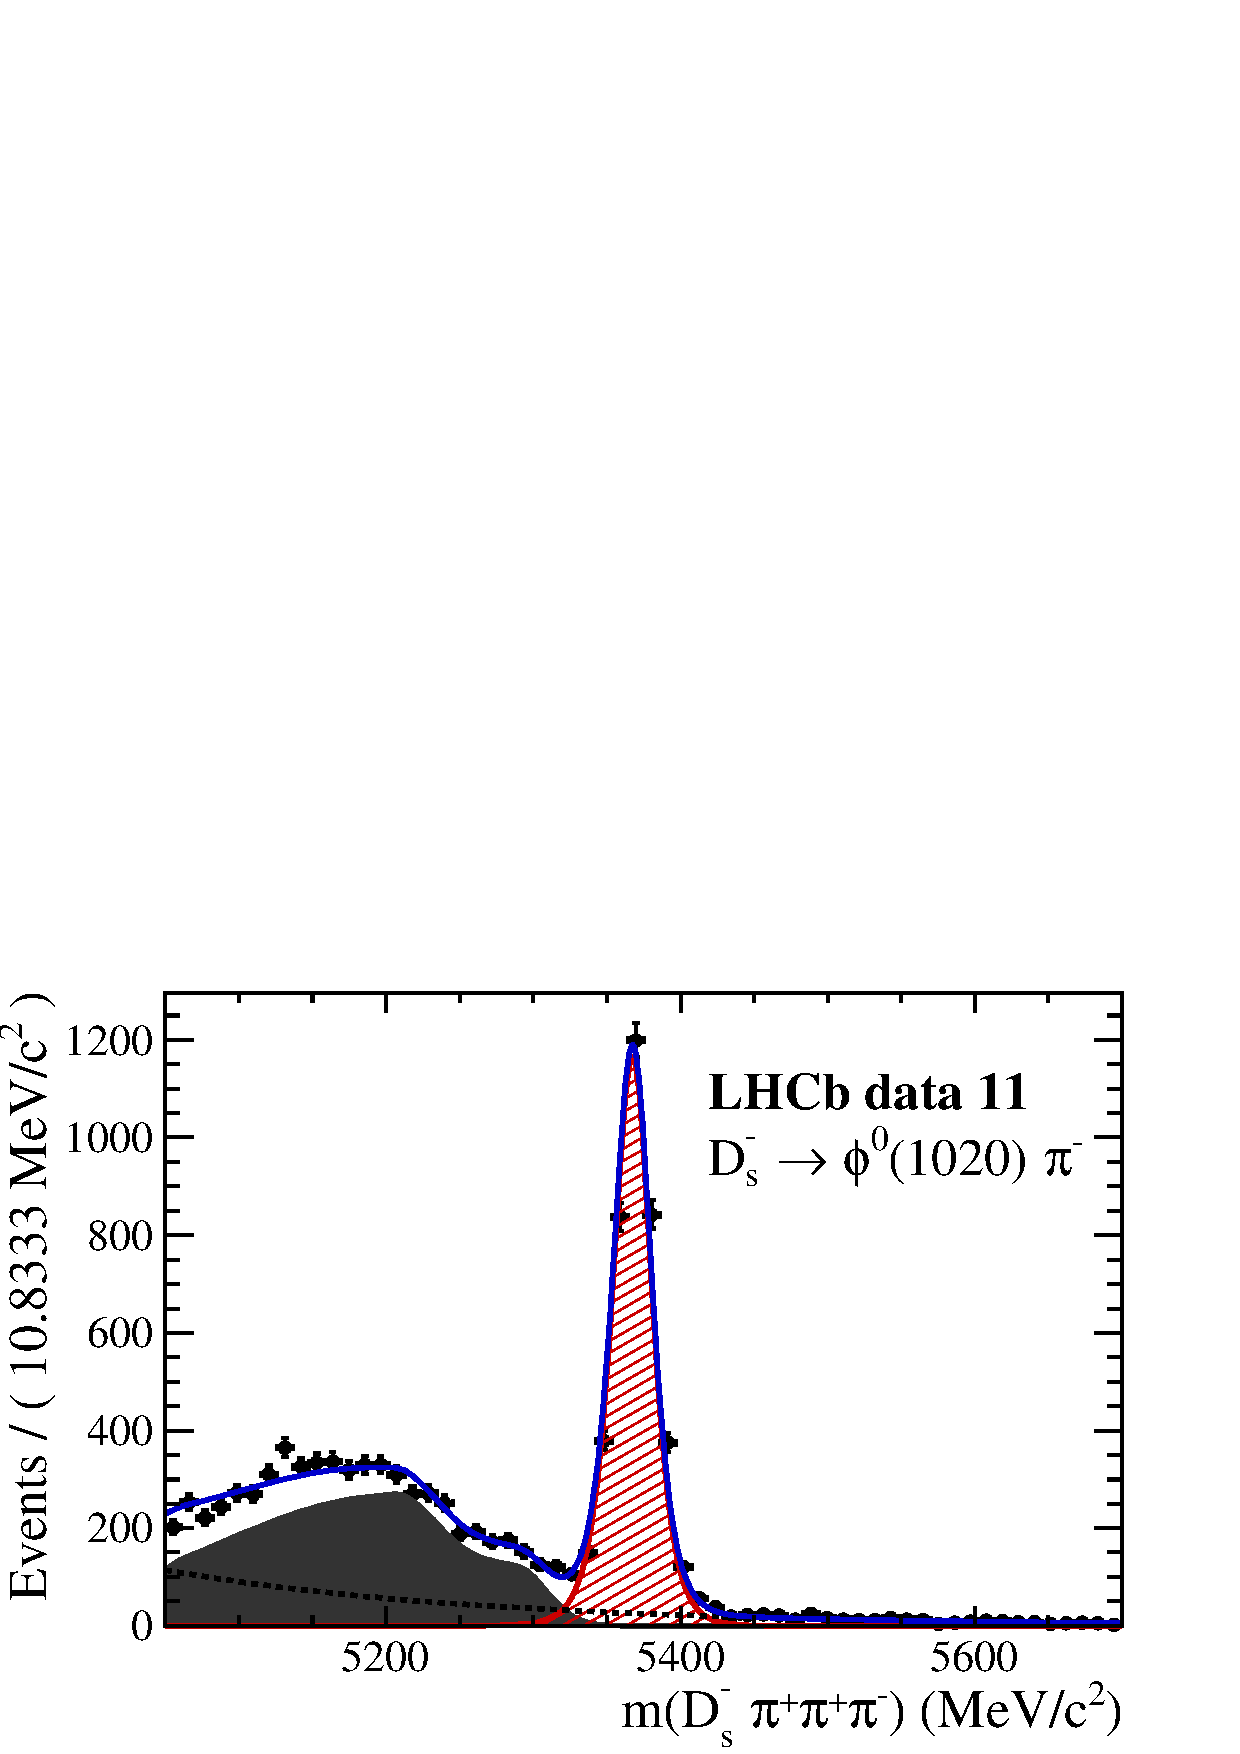
\includegraphics[height=!,width=0.5\textwidth]{figs/MassFit/norm_y11_phipi.pdf}
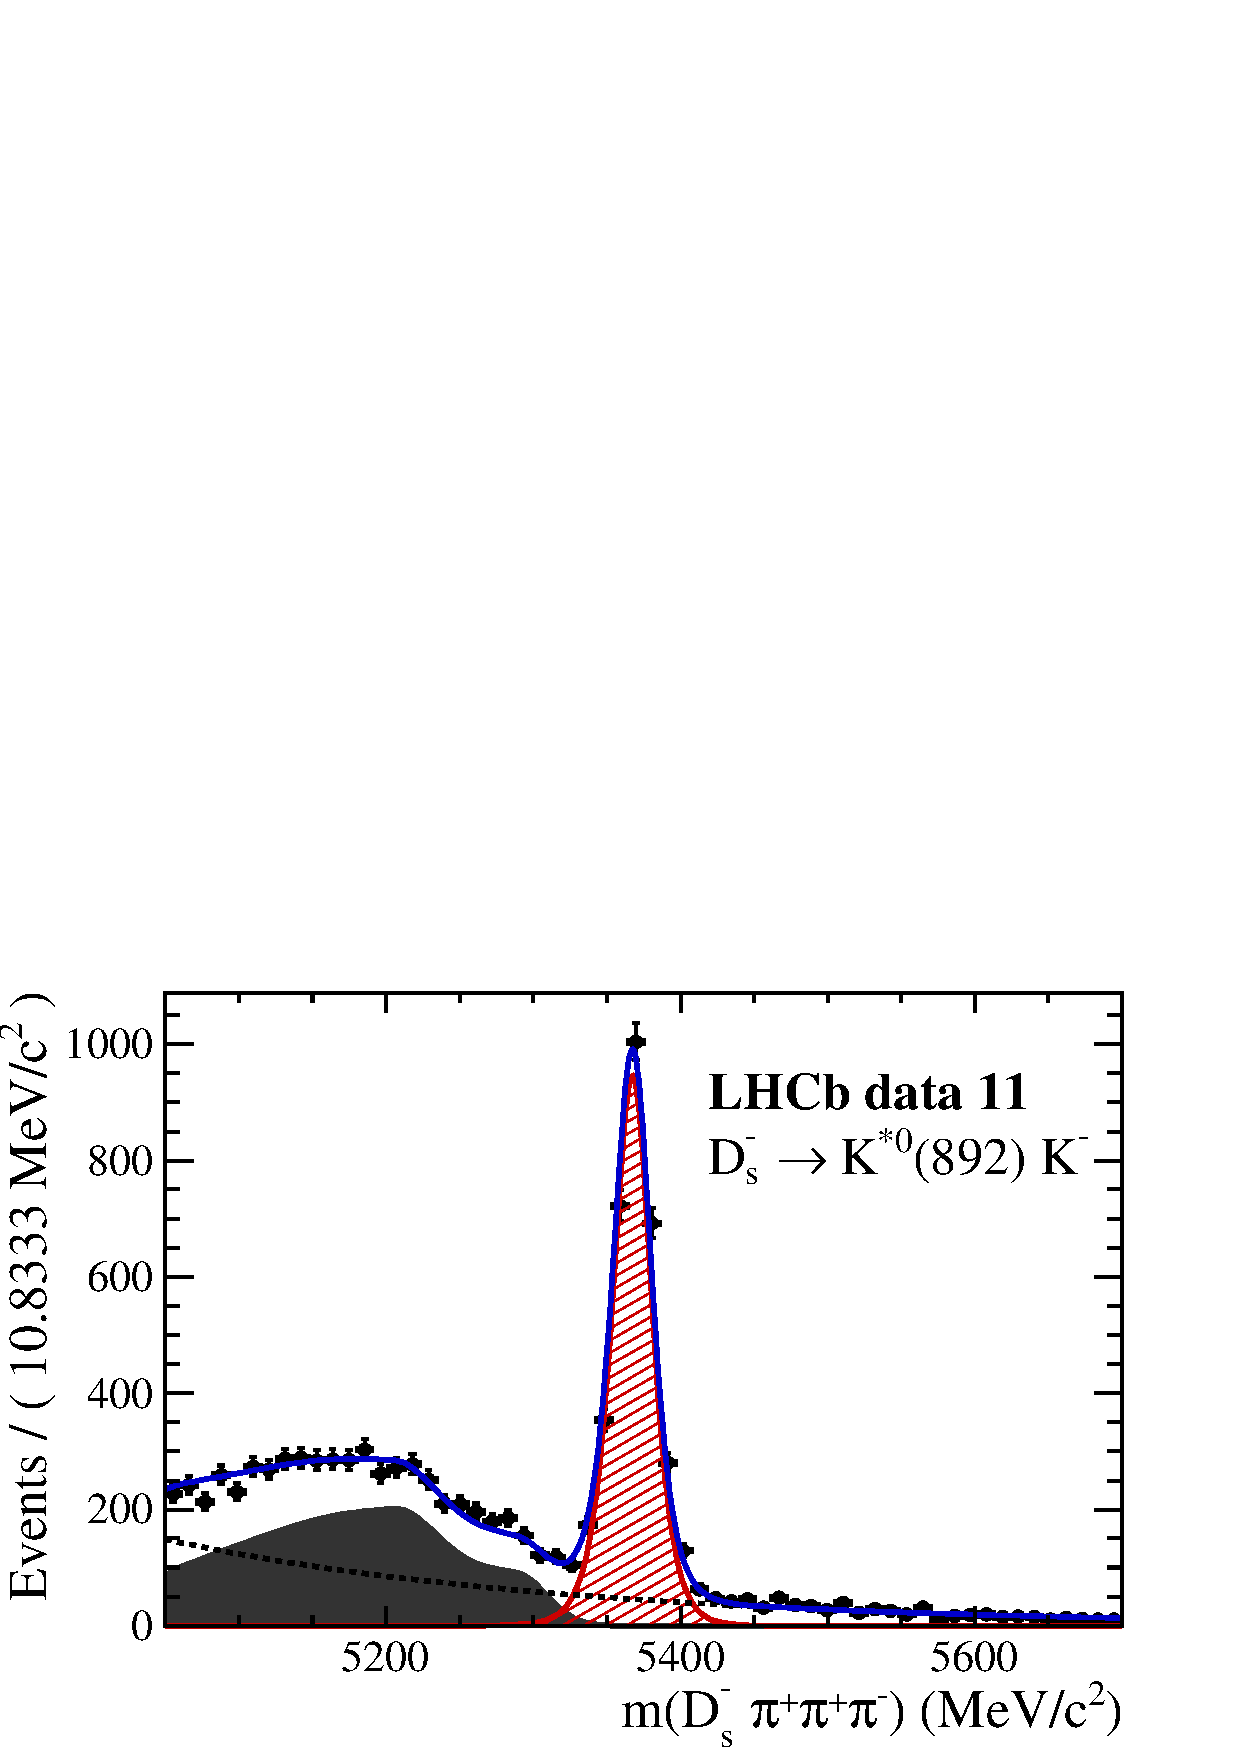
\includegraphics[height=!,width=0.5\textwidth]{figs/MassFit/norm_y11_KsK.pdf}
\includegraphics[height=!,width=0.5\textwidth]{figs/MassFit/norm_y11_KKpi_NR.pdf}
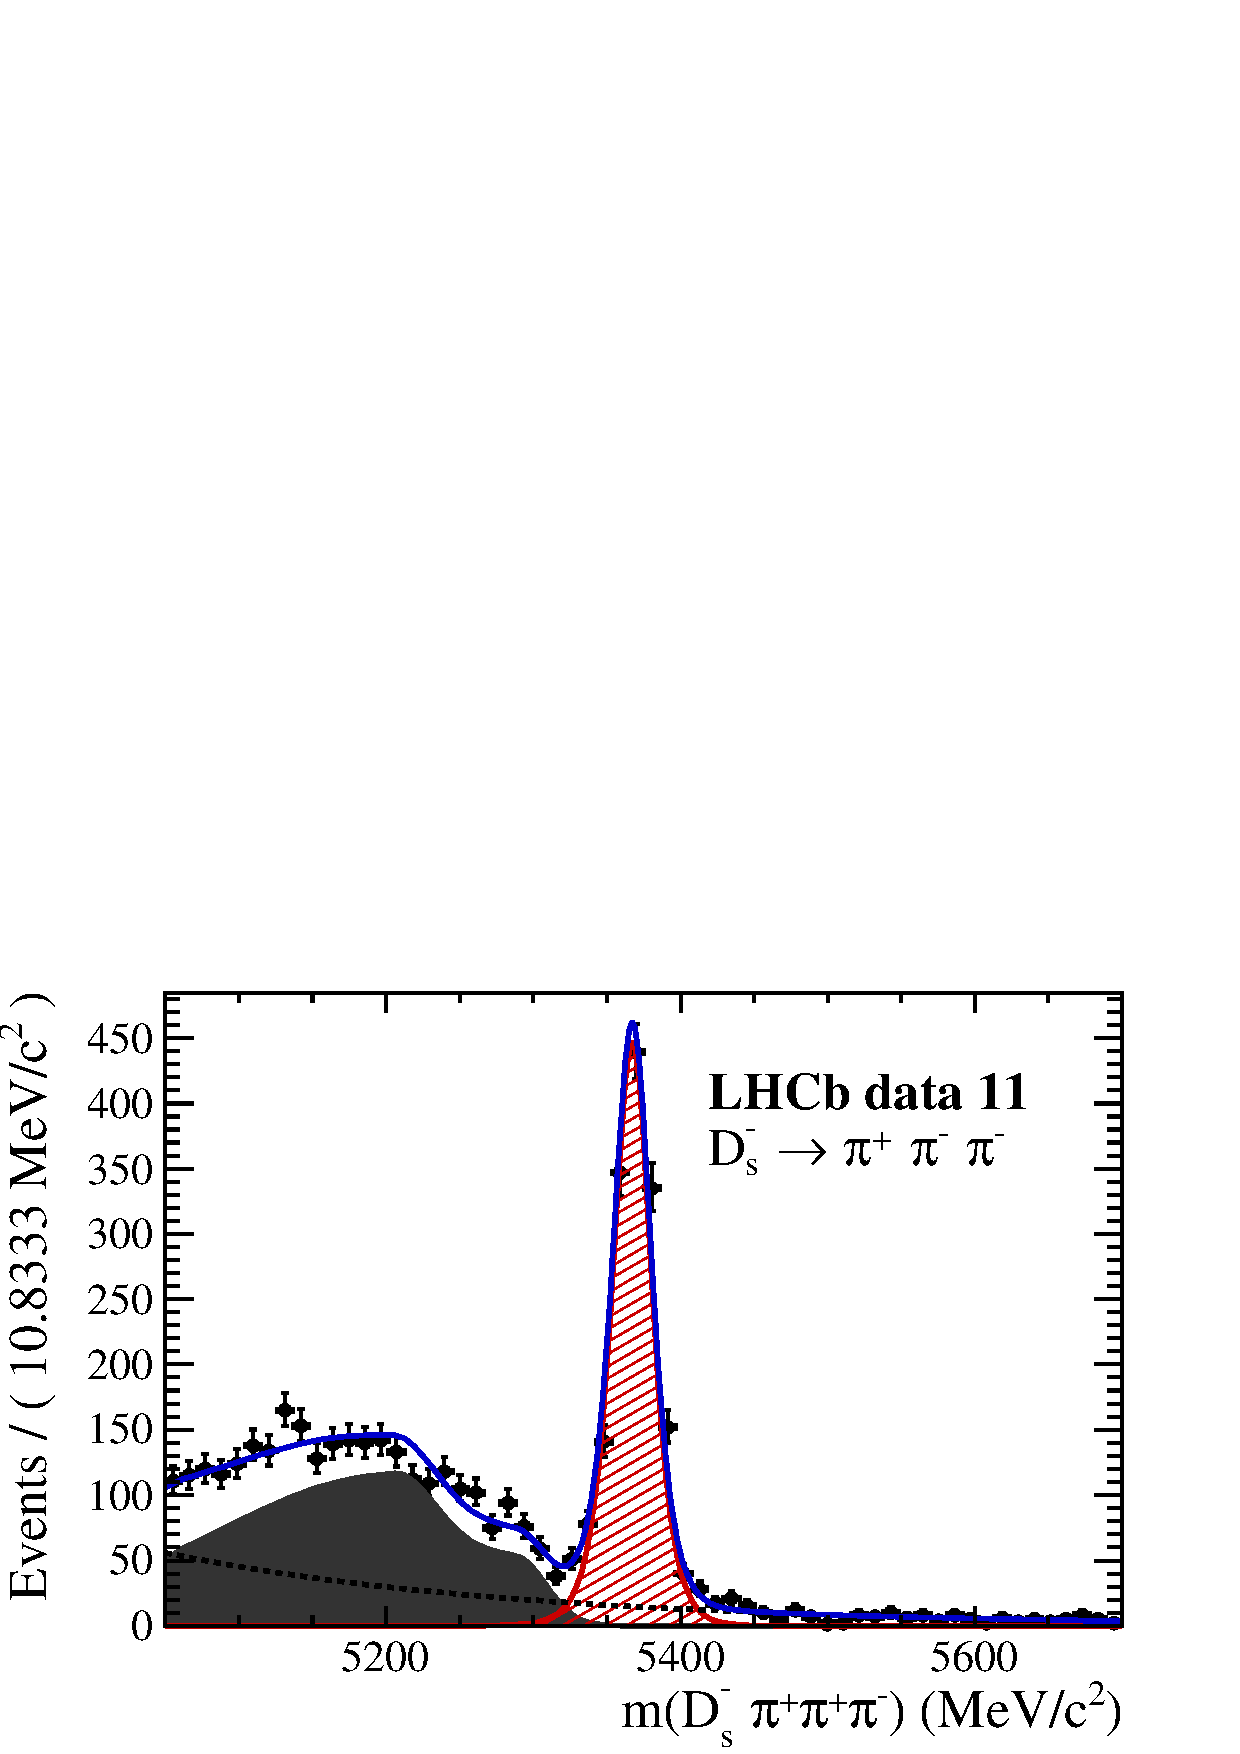
\includegraphics[height=!,width=0.5\textwidth]{figs/MassFit/norm_y11_pipipi.pdf}
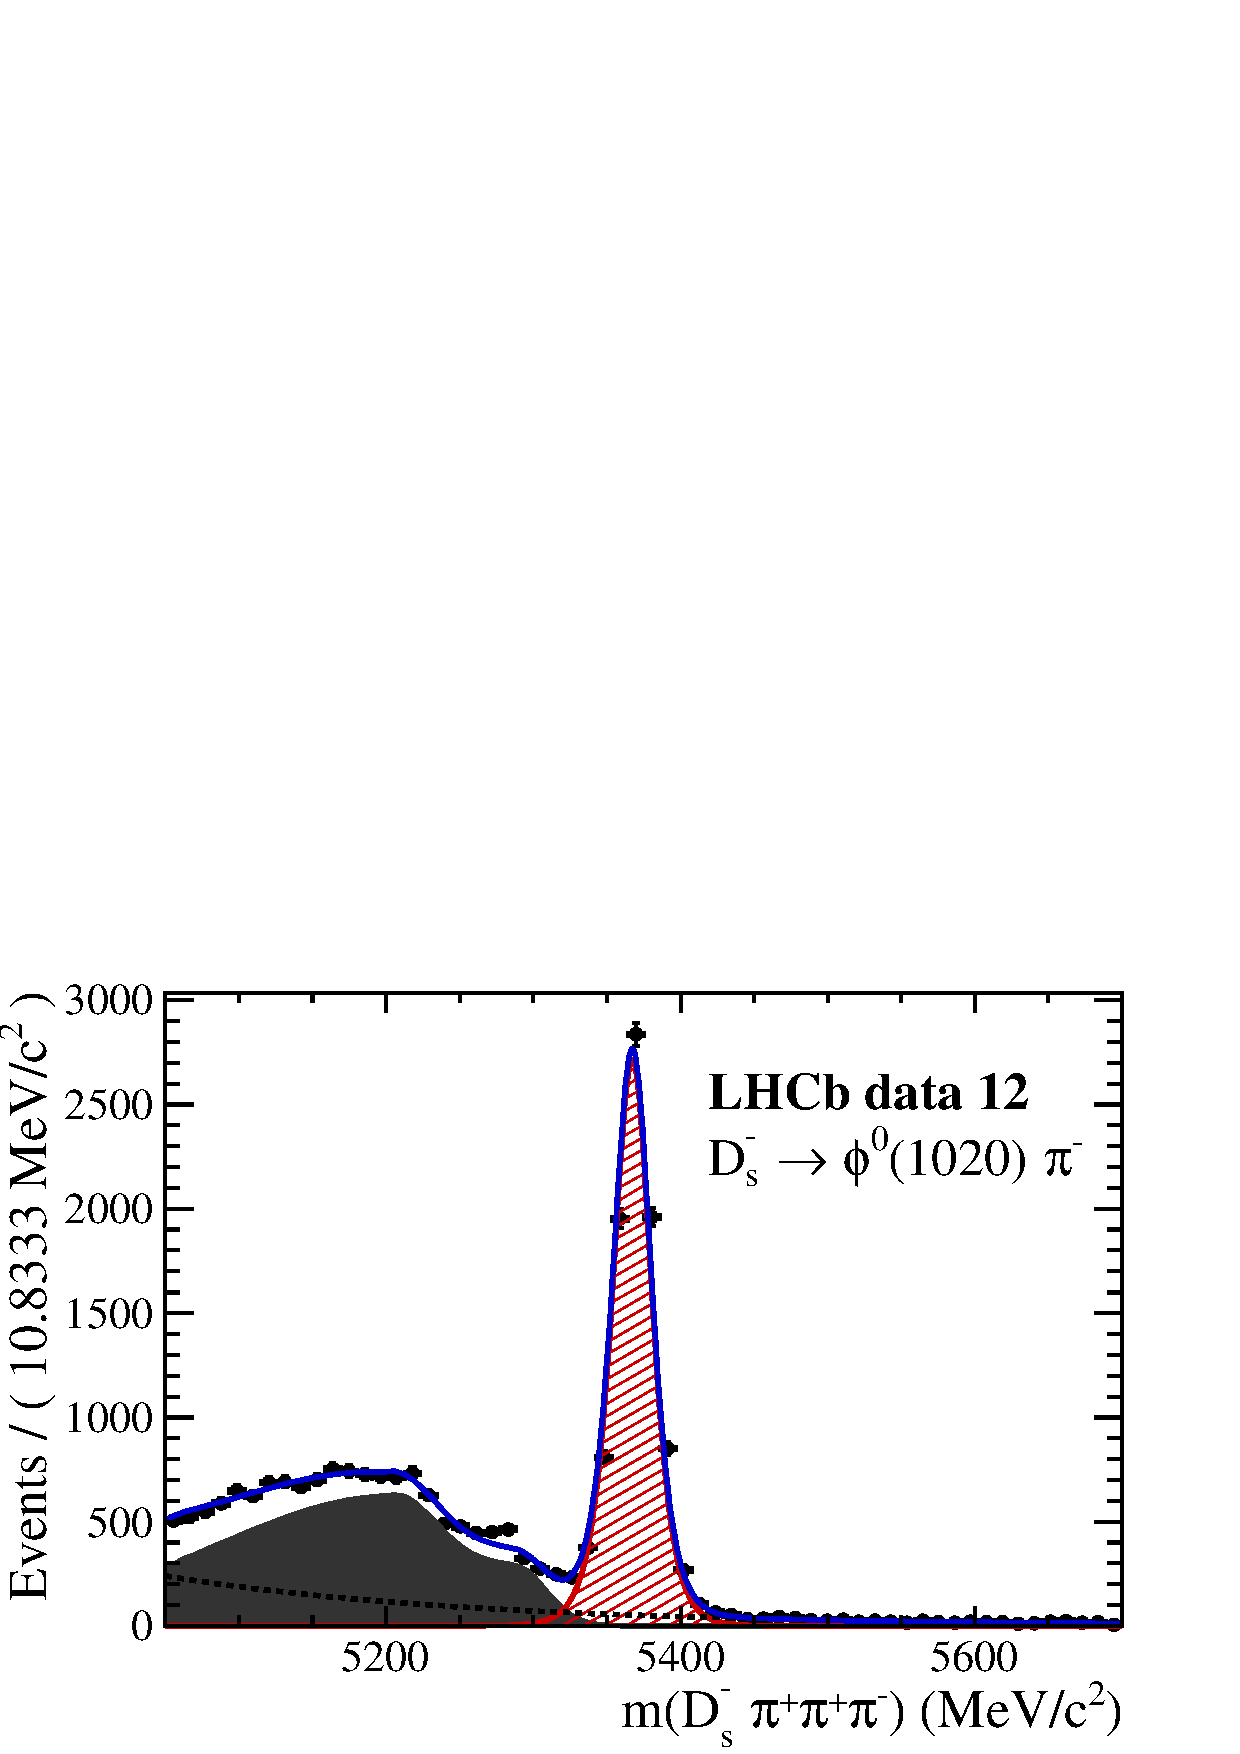
\includegraphics[height=!,width=0.5\textwidth]{figs/MassFit/norm_y12_phipi.pdf}
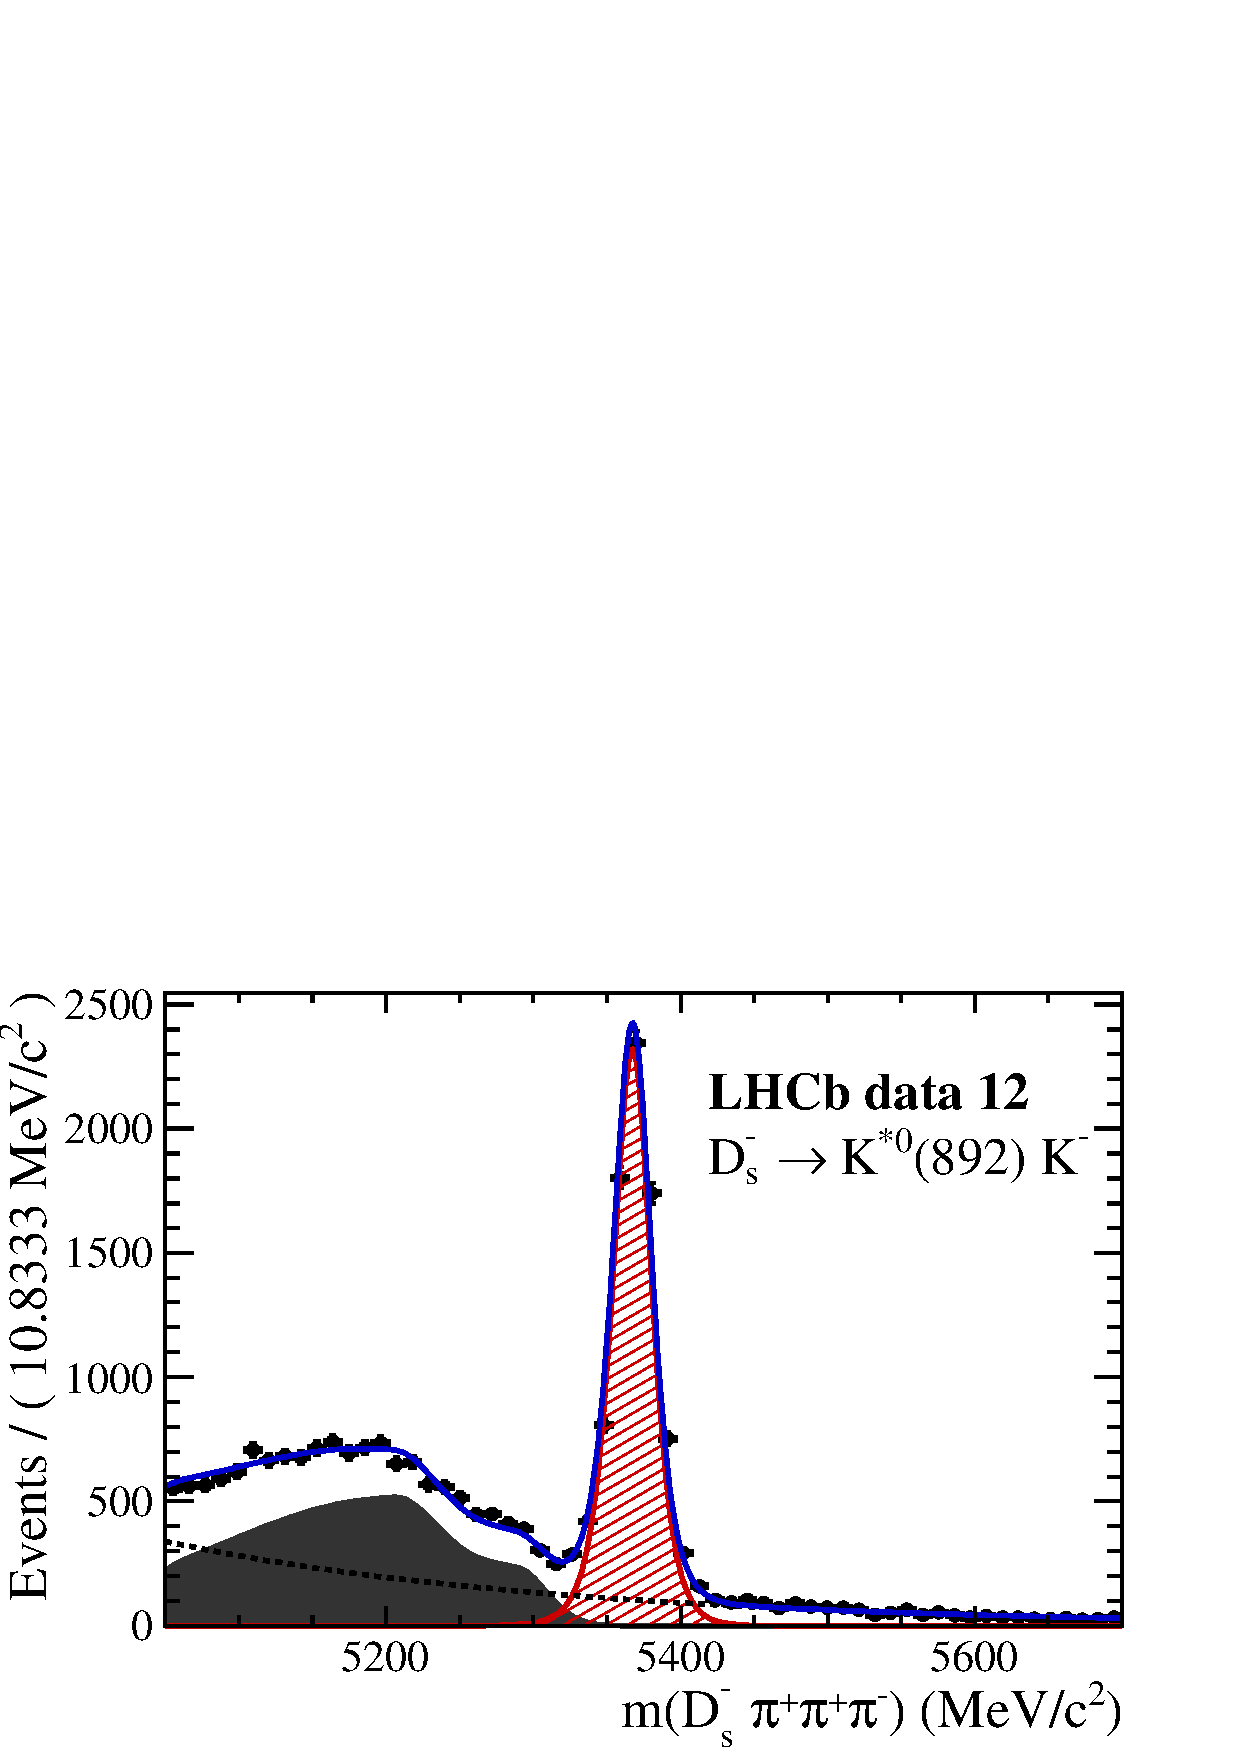
\includegraphics[height=!,width=0.5\textwidth]{figs/MassFit/norm_y12_KsK.pdf}
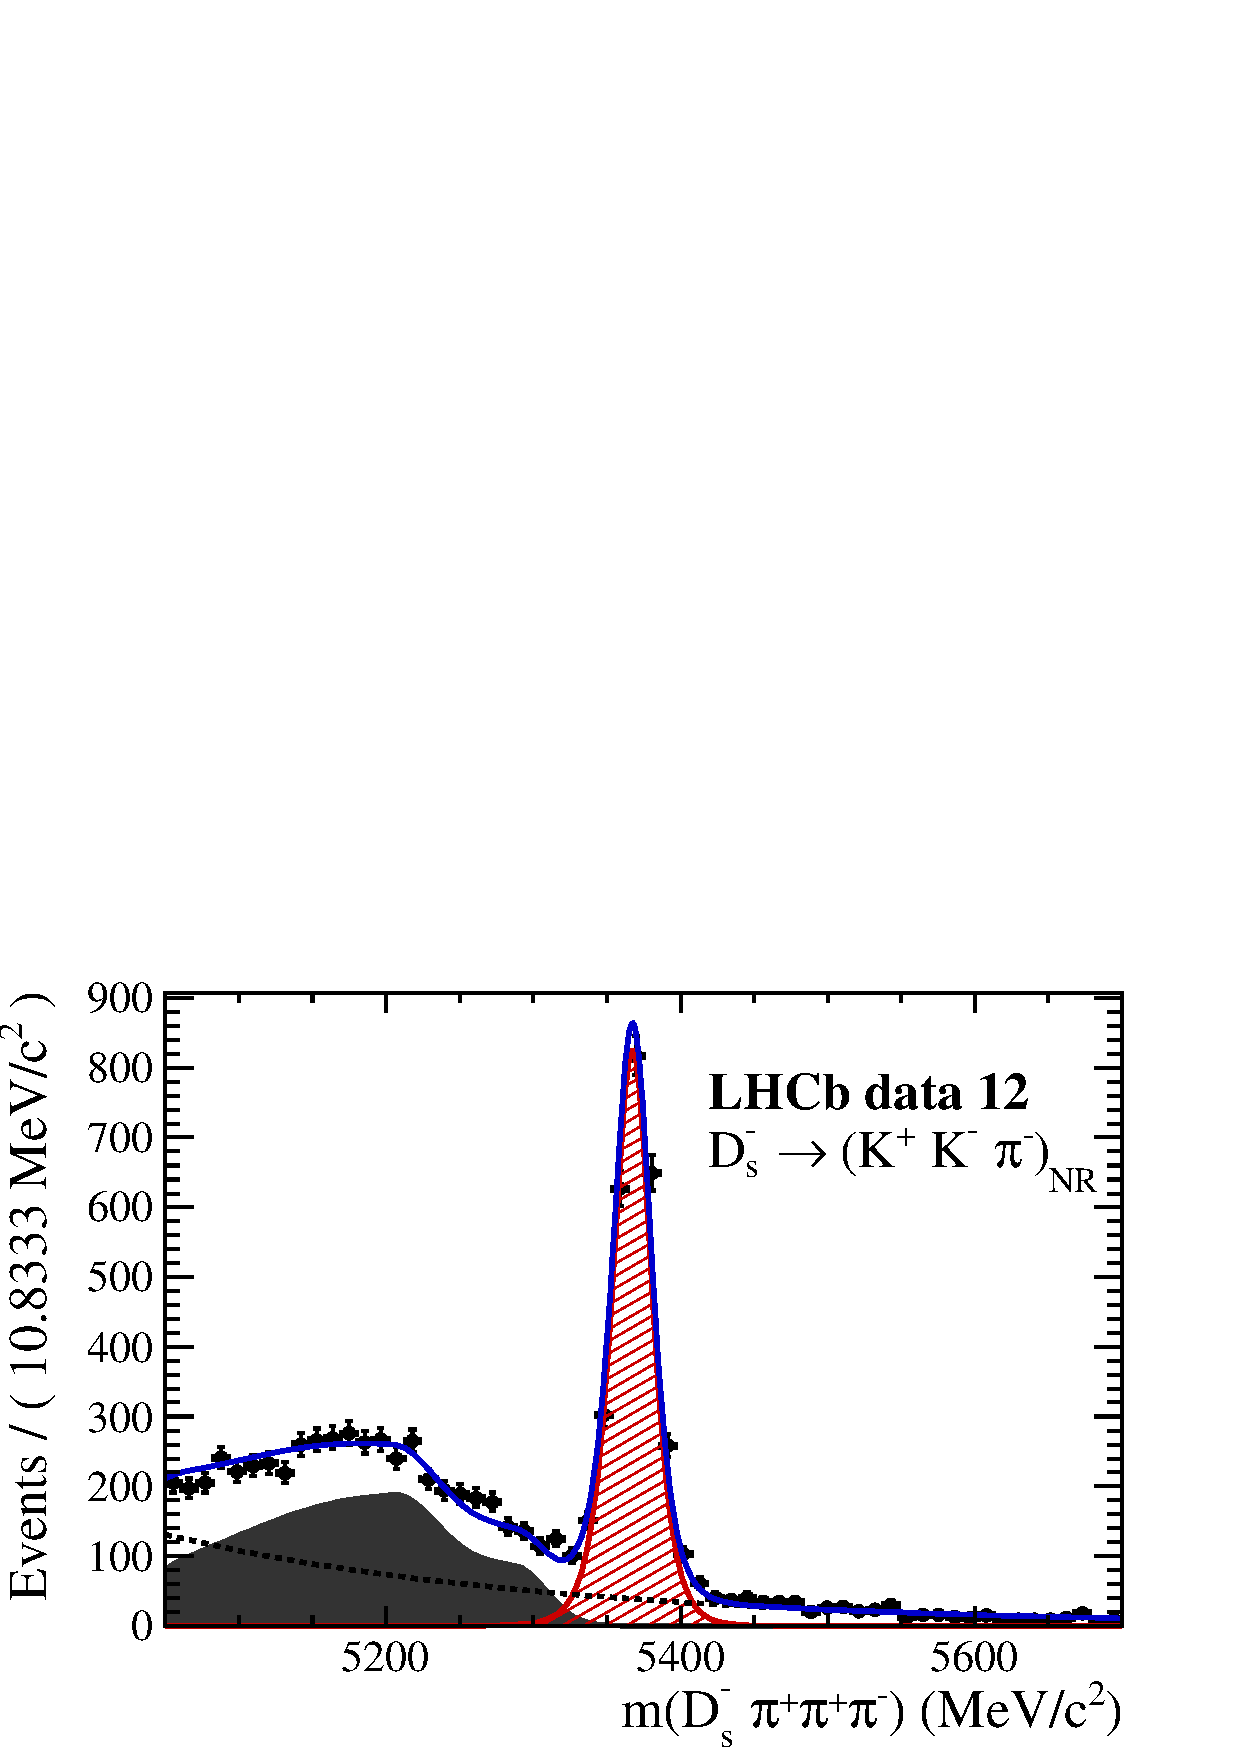
\includegraphics[height=!,width=0.5\textwidth]{figs/MassFit/norm_y12_KKpi_NR.pdf}
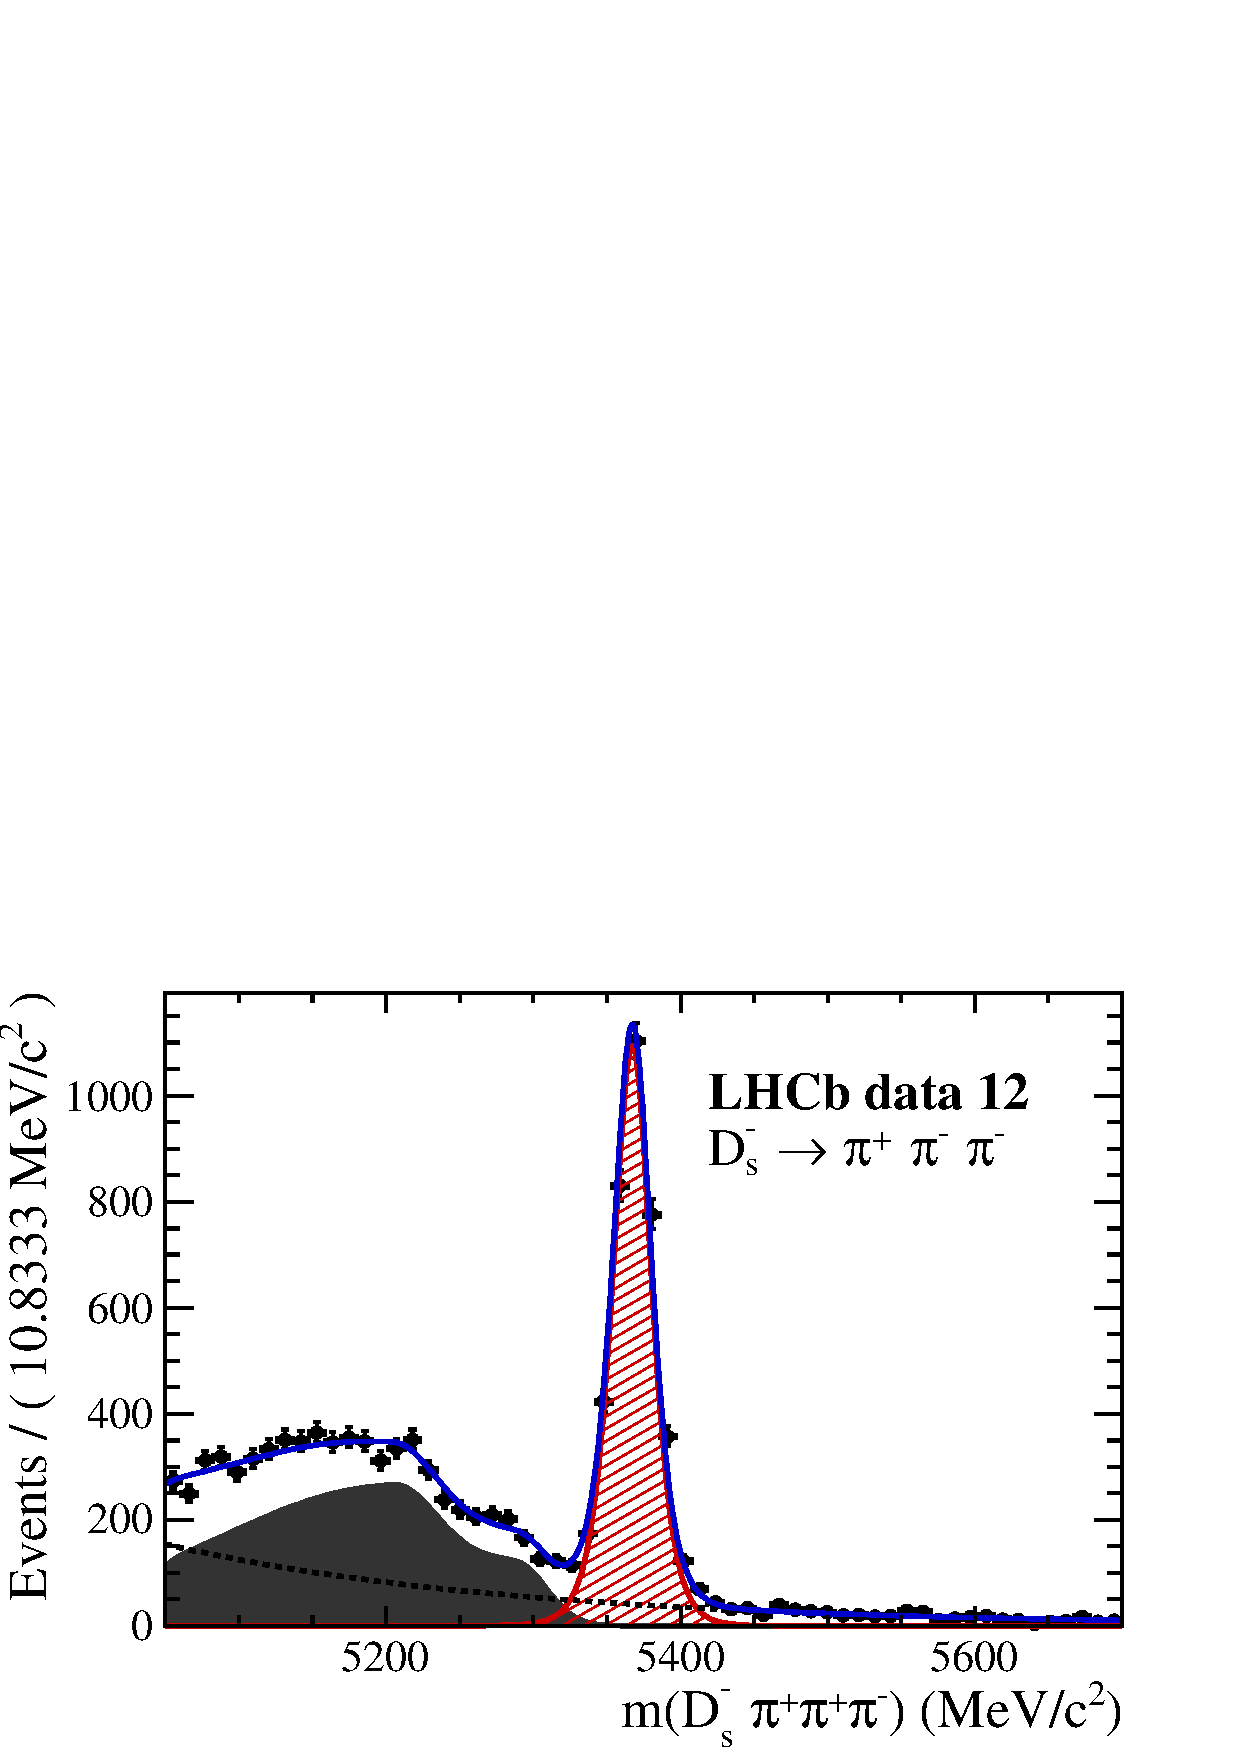
\includegraphics[height=!,width=0.5\textwidth]{figs/MassFit/norm_y12_pipipi.pdf}
\caption{Invariant mass distributions of $\Bs\to\Ds\pion\pion\pion$ candidates, ordered by $\Ds$ final state, for Run1 data.
The fit described in \ref{subsec: NormFit} is overlaid.}
\label{fig:massfits_norm_Run1}
\end{figure}

\clearpage

\begin{figure}[h]
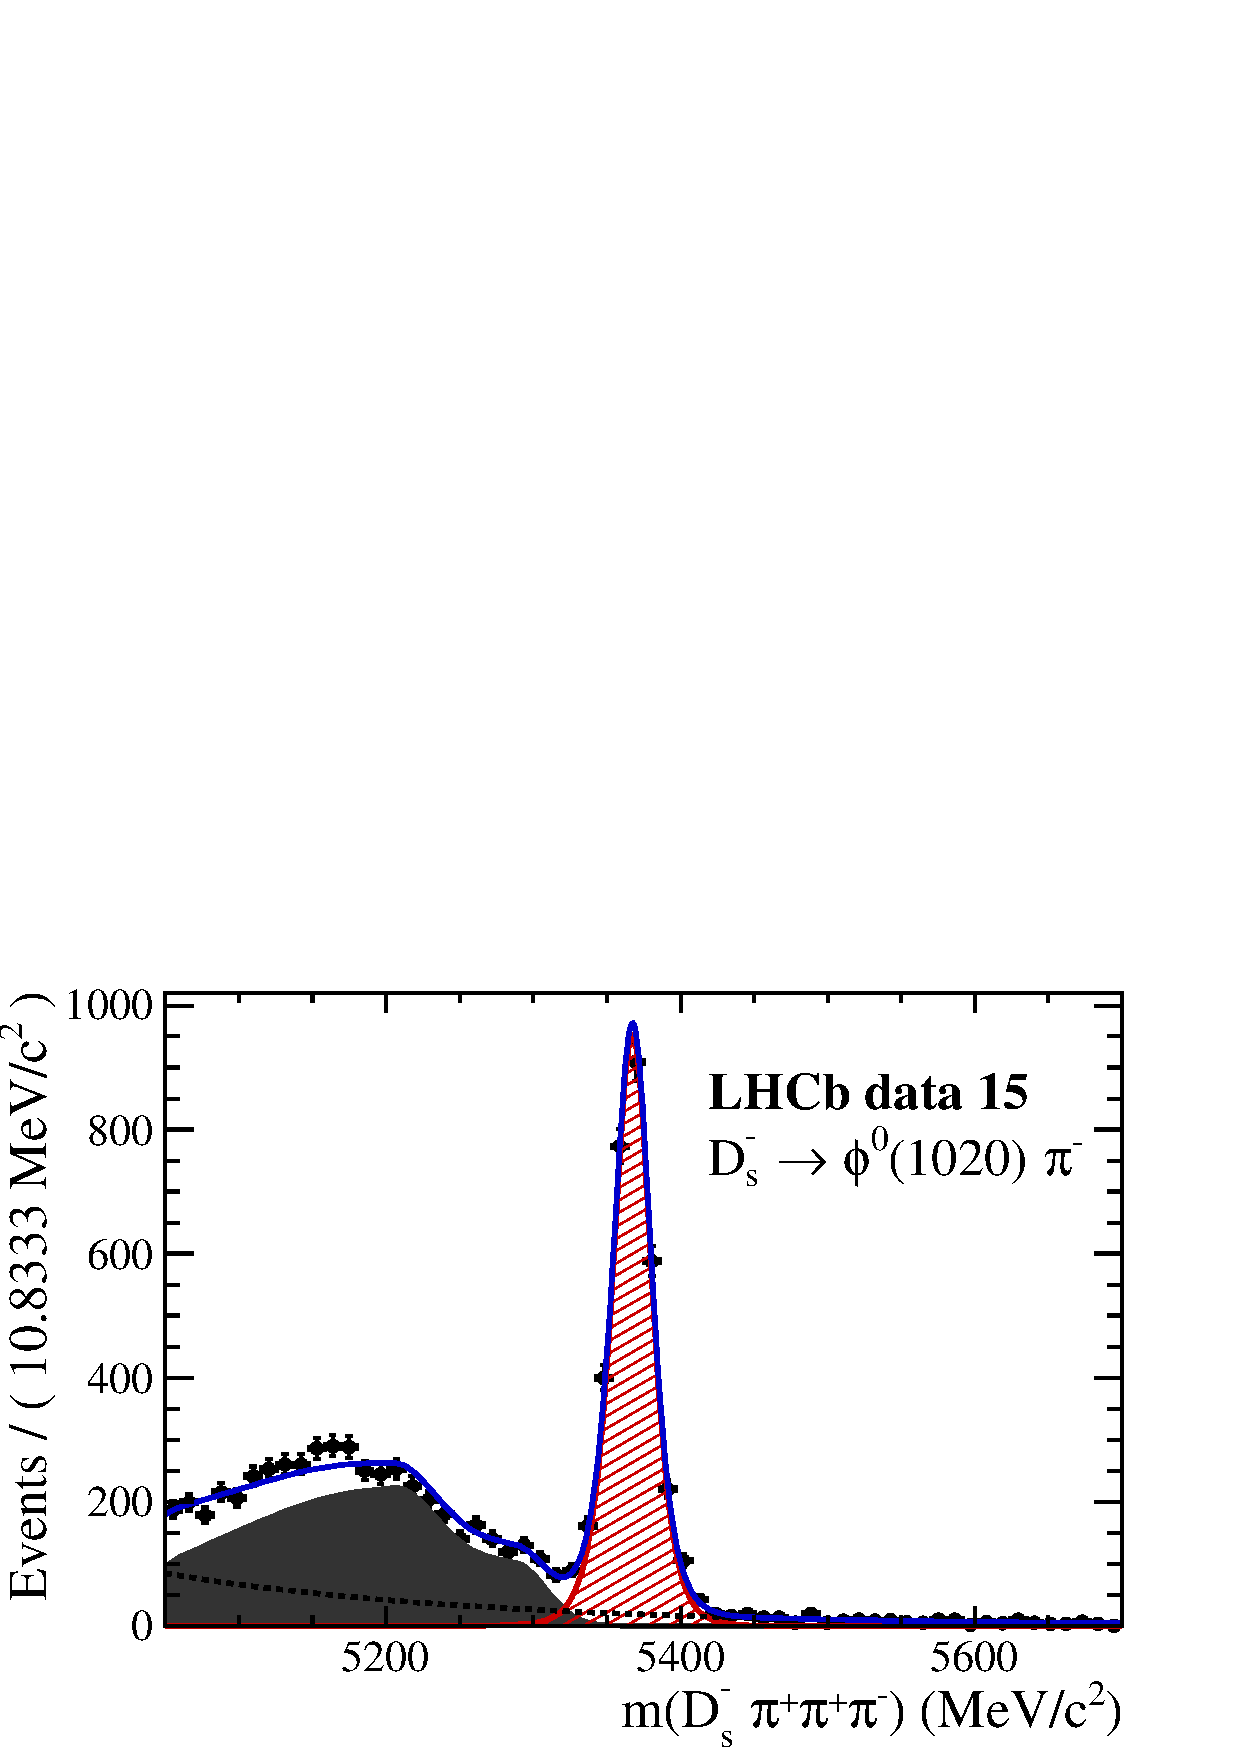
\includegraphics[height=!,width=0.5\textwidth]{figs/MassFit/norm_y15_phipi.pdf}
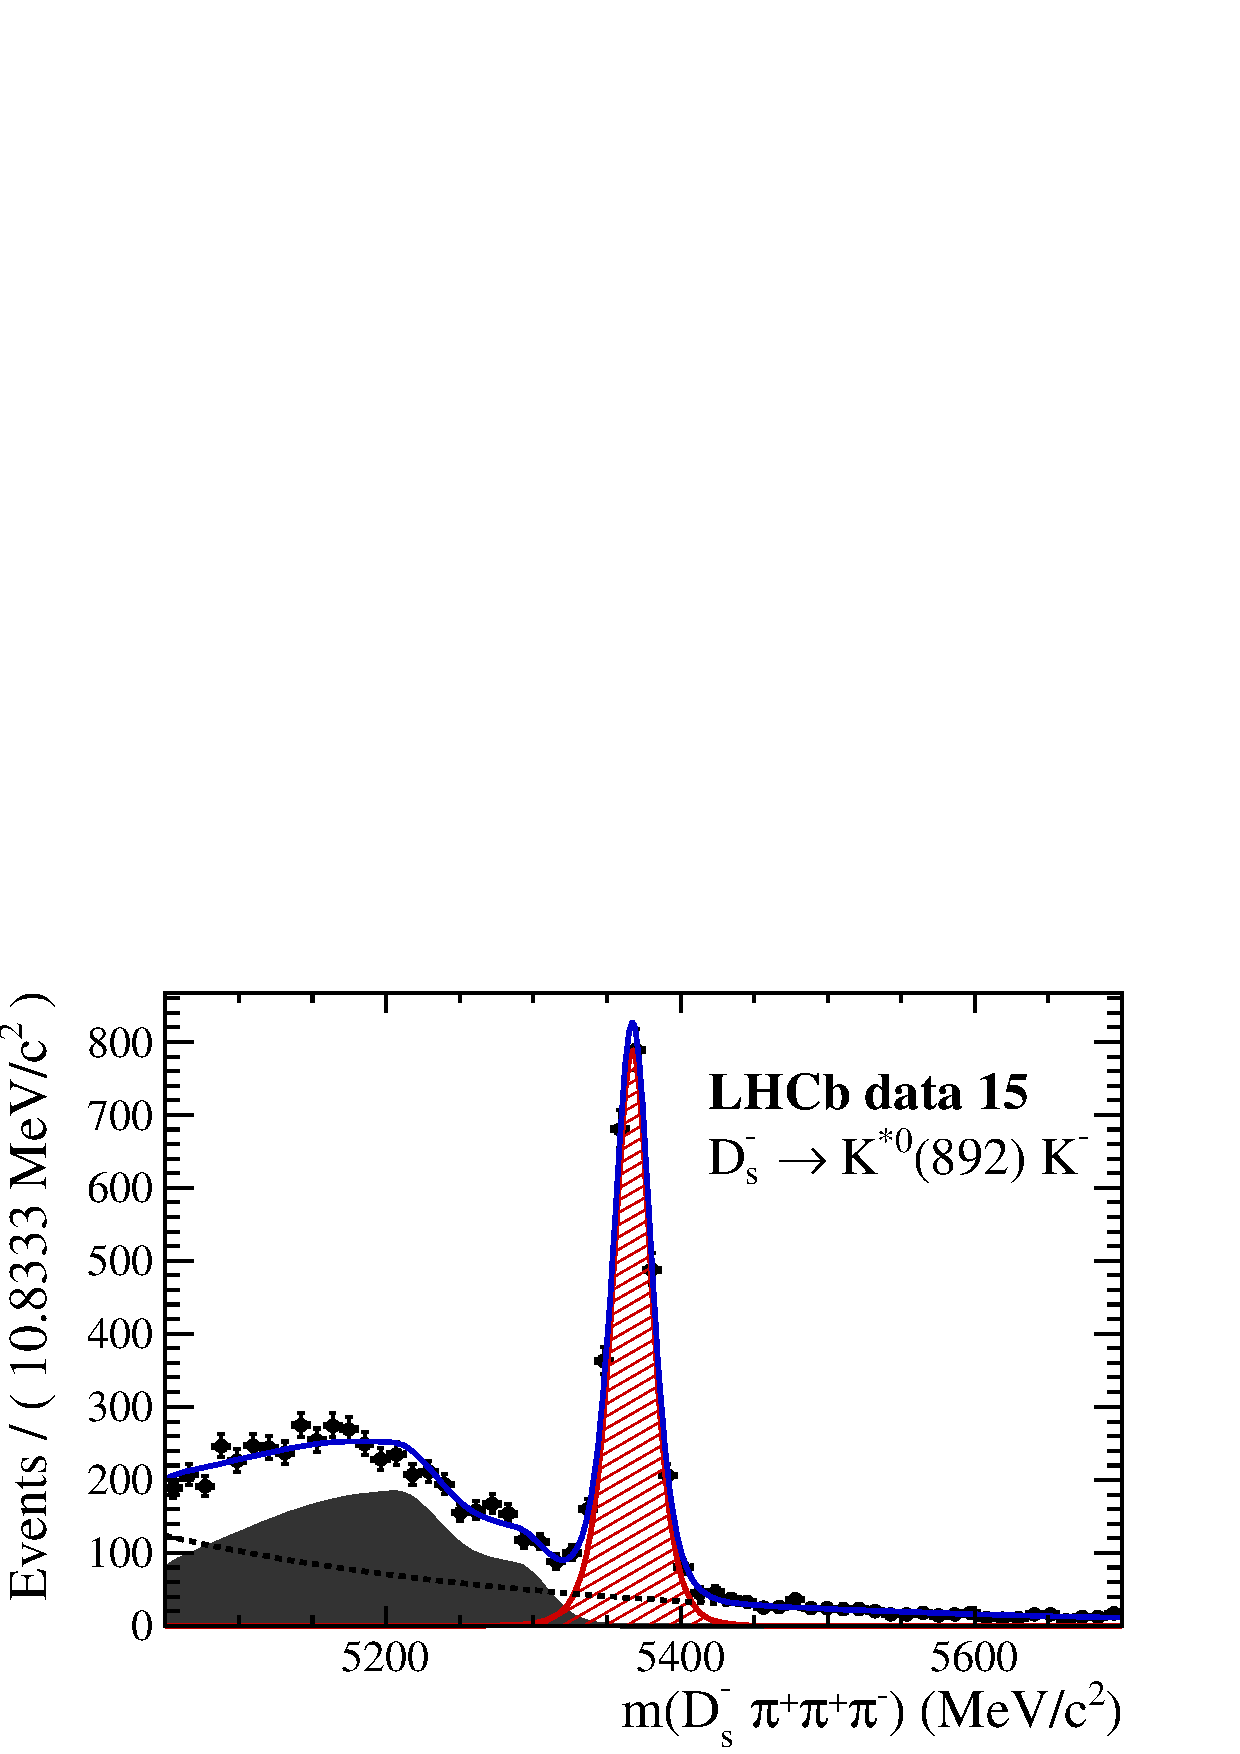
\includegraphics[height=!,width=0.5\textwidth]{figs/MassFit/norm_y15_KsK.pdf}
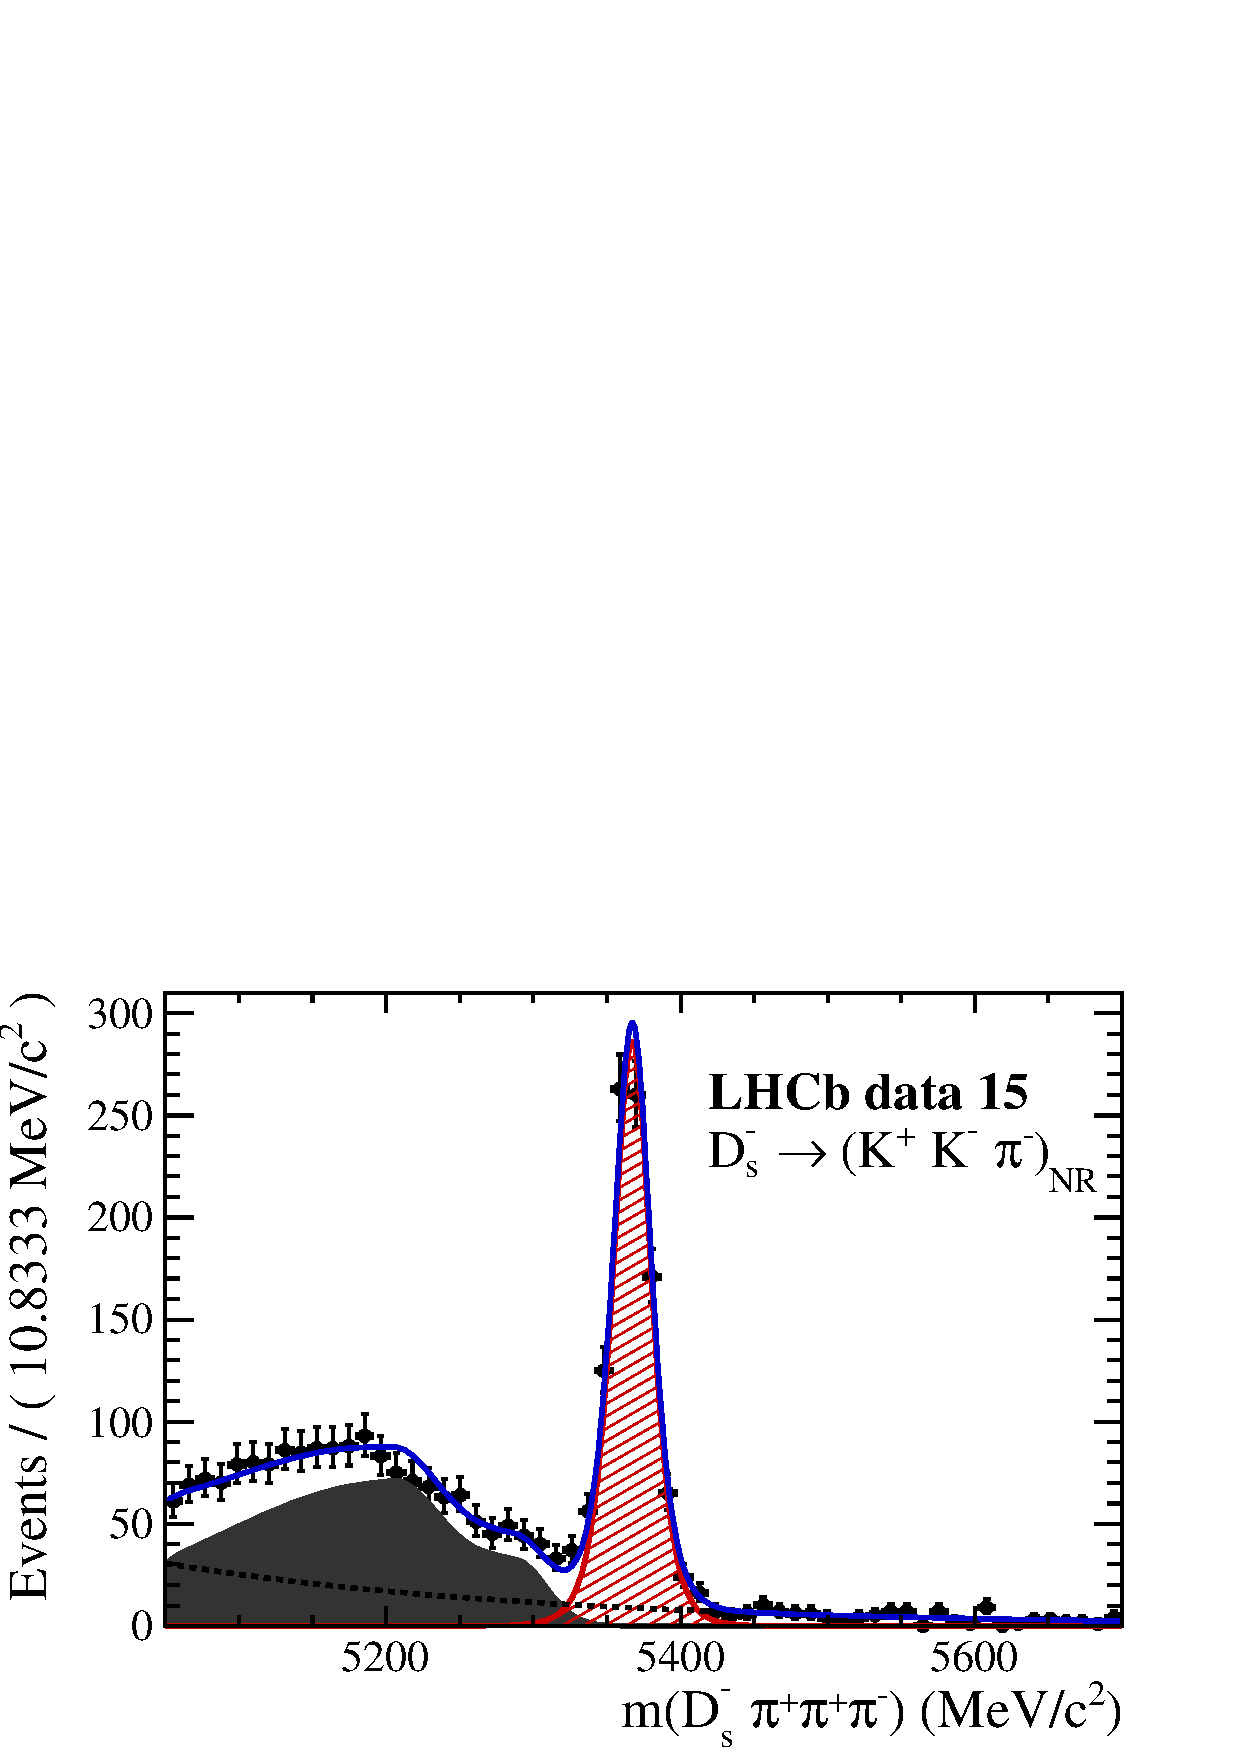
\includegraphics[height=!,width=0.5\textwidth]{figs/MassFit/norm_y15_KKpi_NR.pdf}
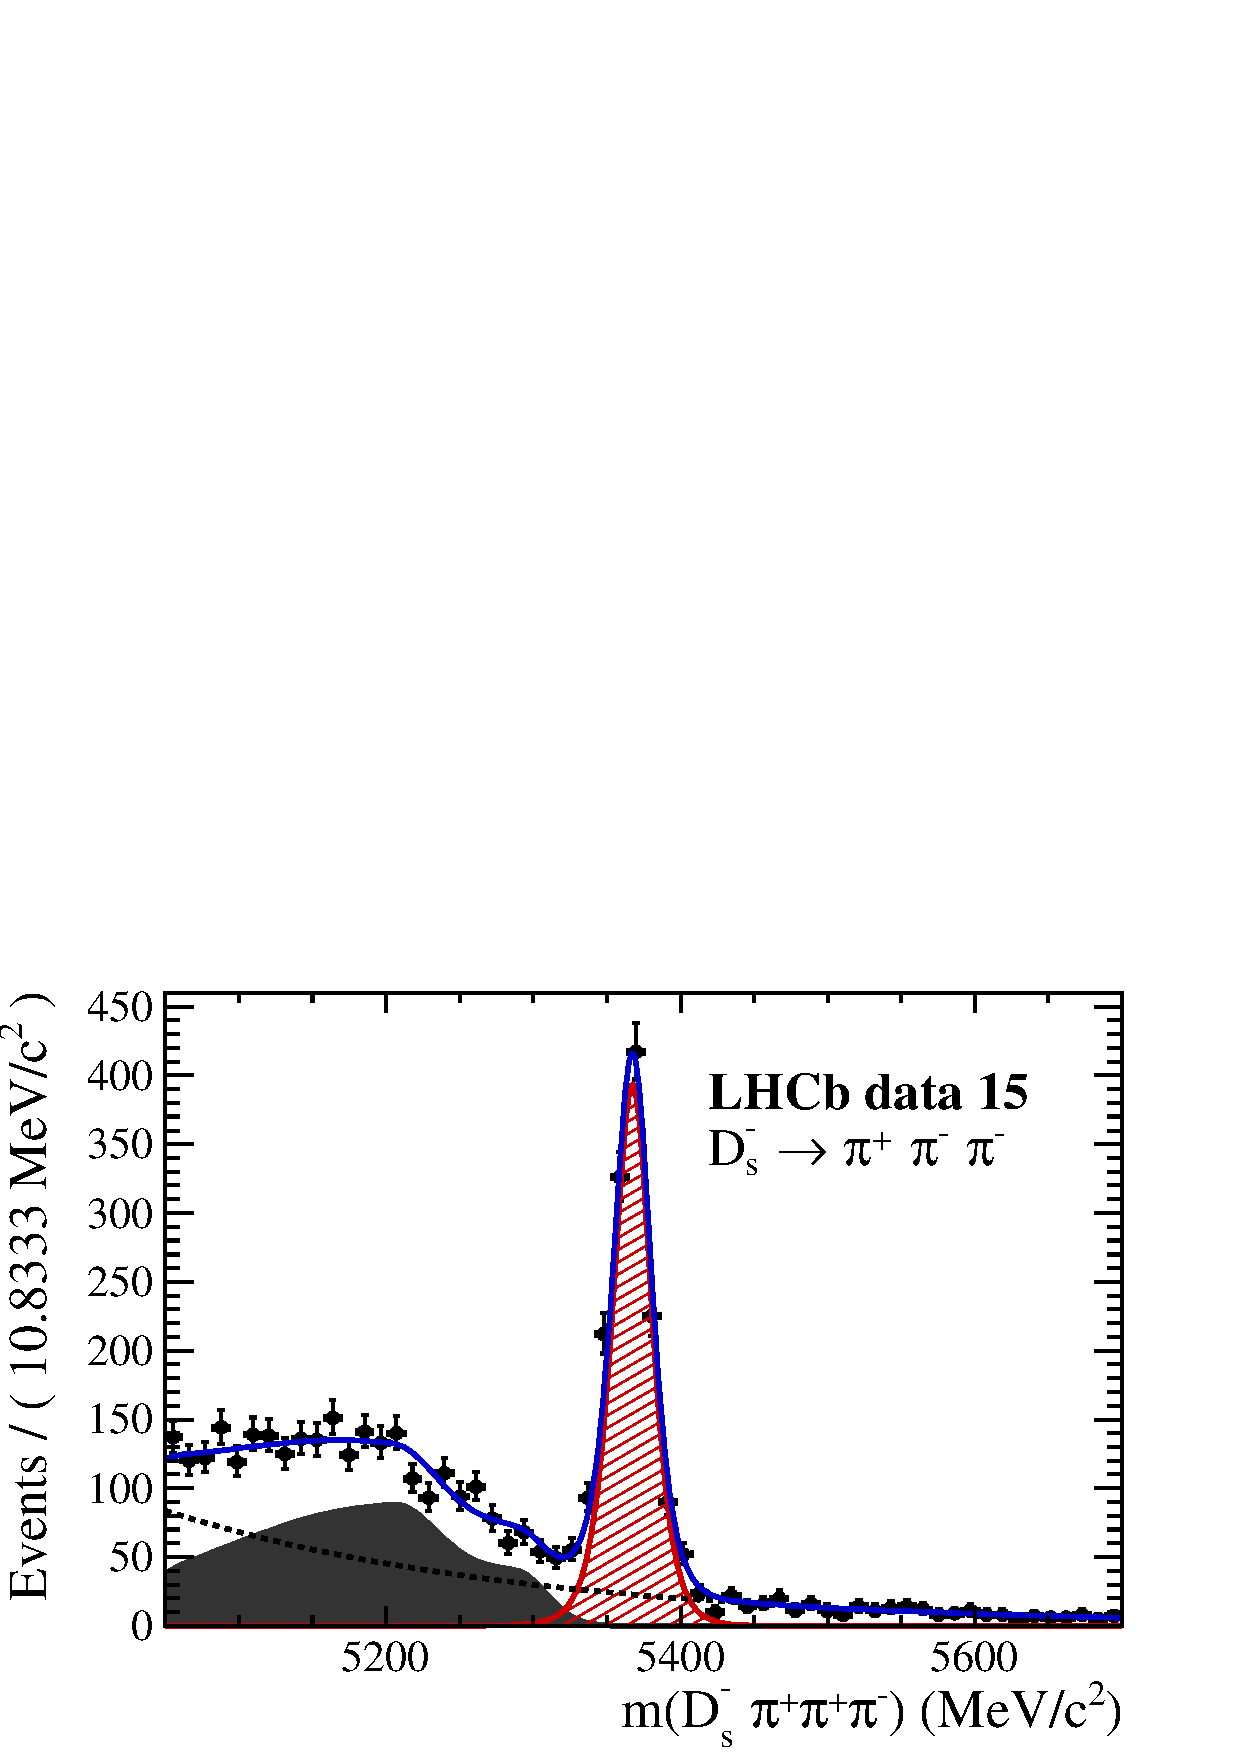
\includegraphics[height=!,width=0.5\textwidth]{figs/MassFit/norm_y15_pipipi.pdf}
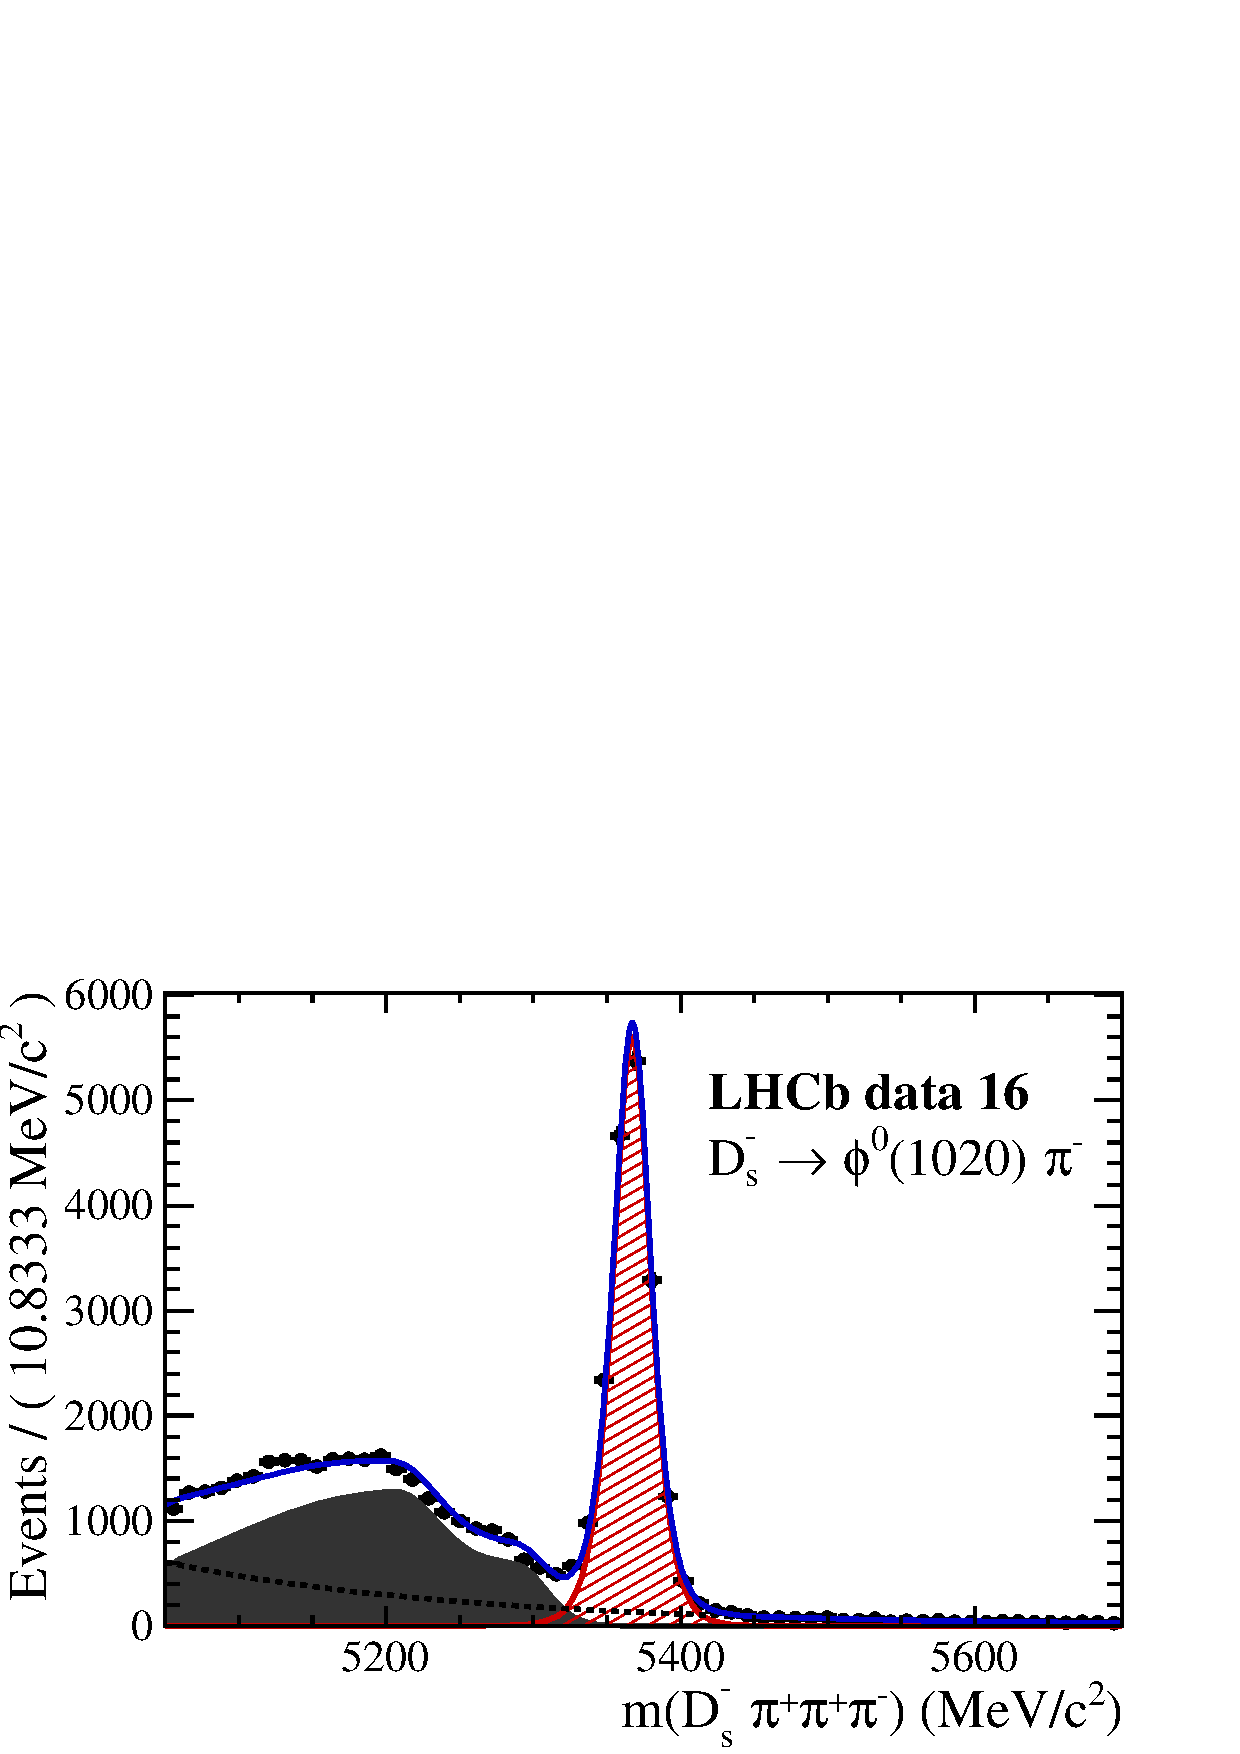
\includegraphics[height=!,width=0.5\textwidth]{figs/MassFit/norm_y16_phipi.pdf}
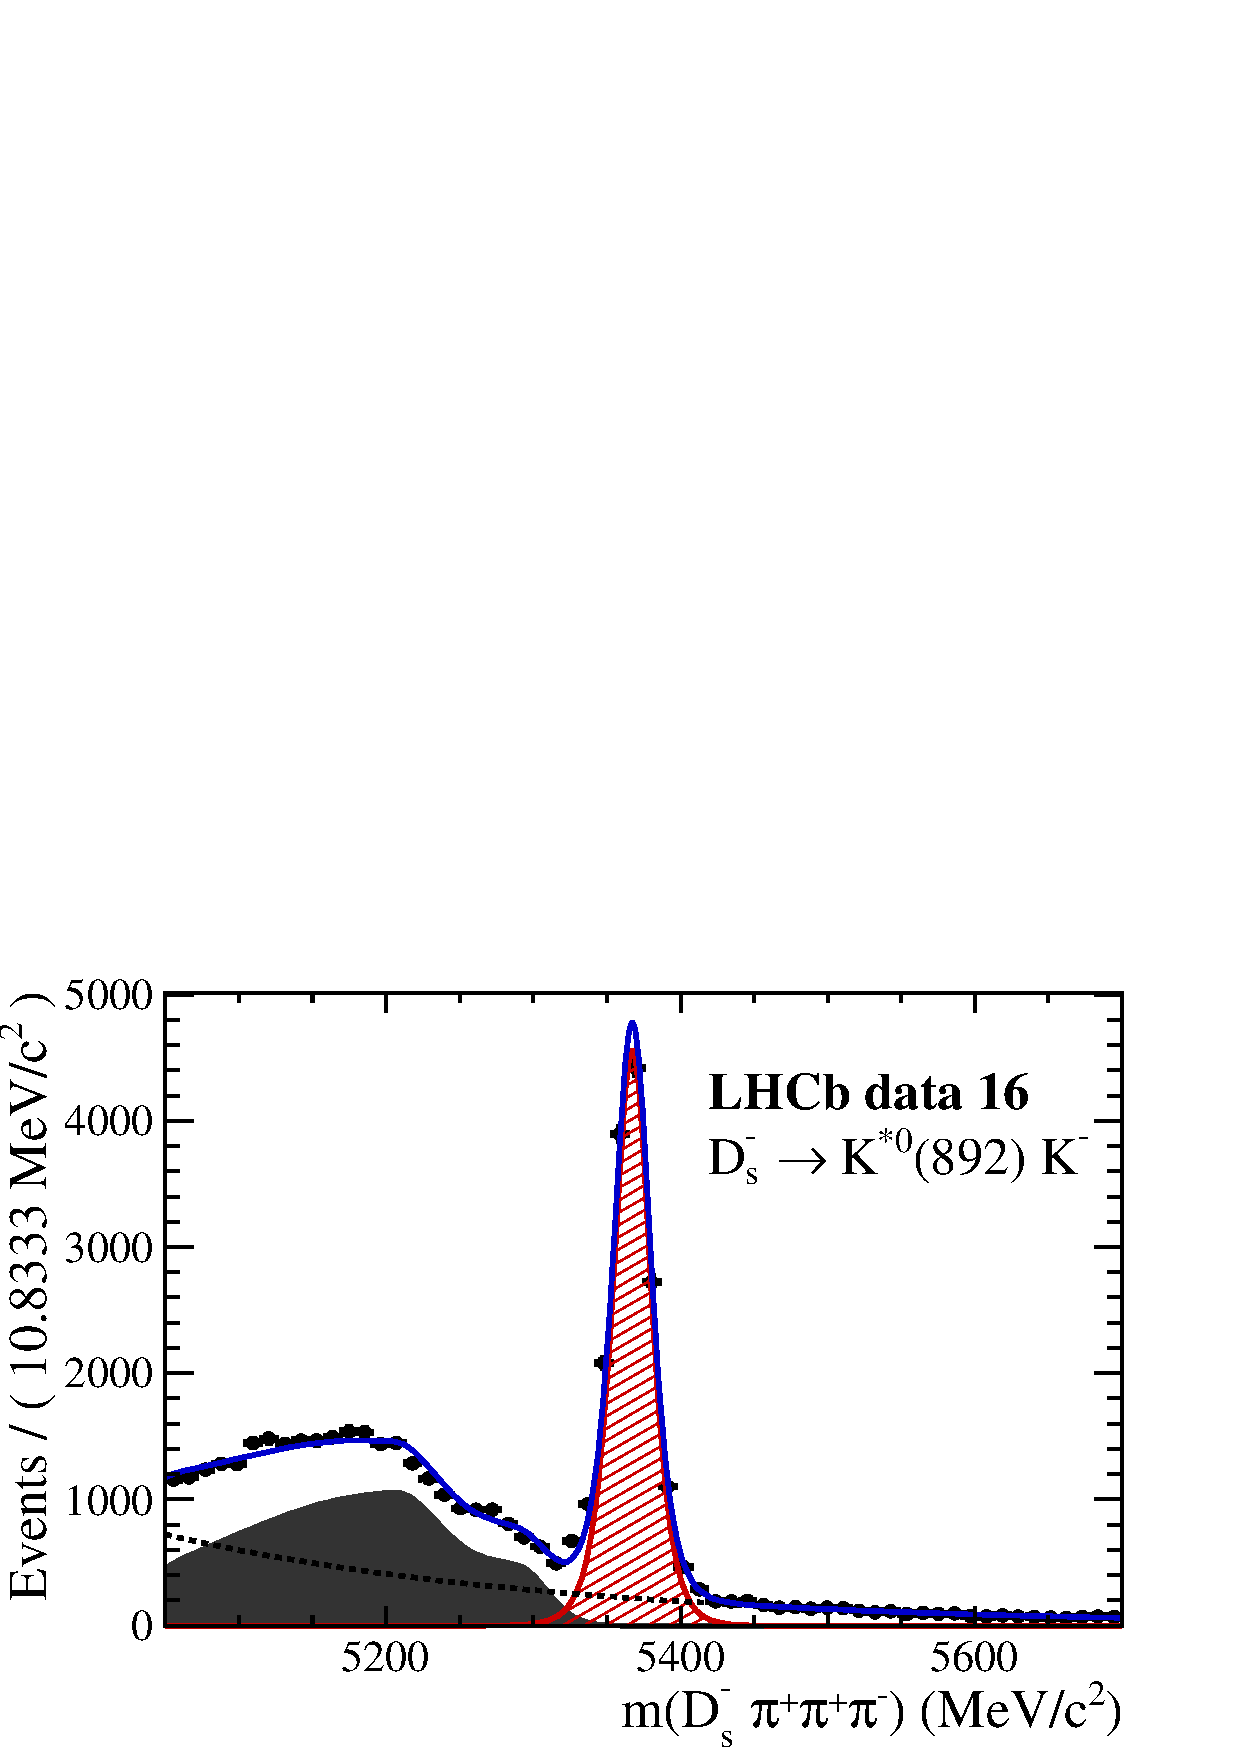
\includegraphics[height=!,width=0.5\textwidth]{figs/MassFit/norm_y16_KsK.pdf}
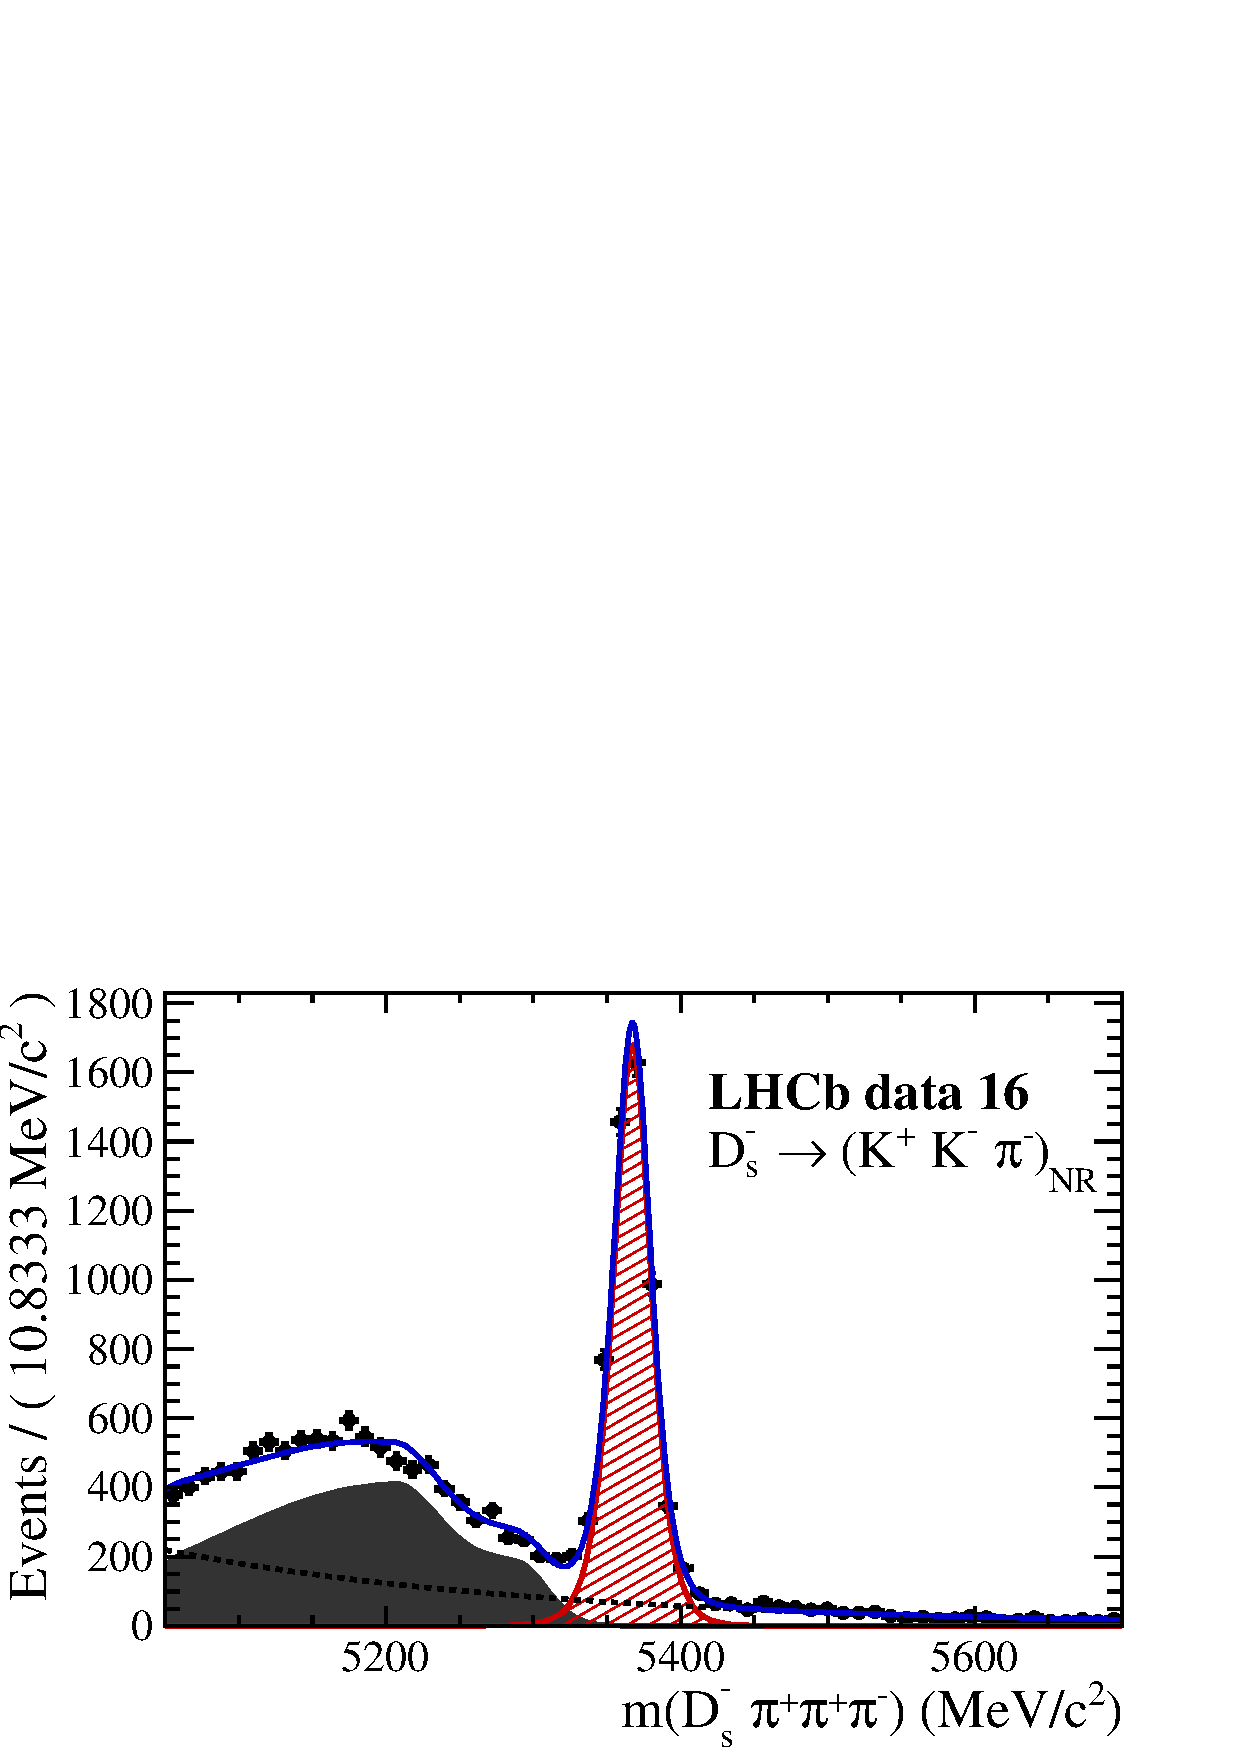
\includegraphics[height=!,width=0.5\textwidth]{figs/MassFit/norm_y16_KKpi_NR.pdf}
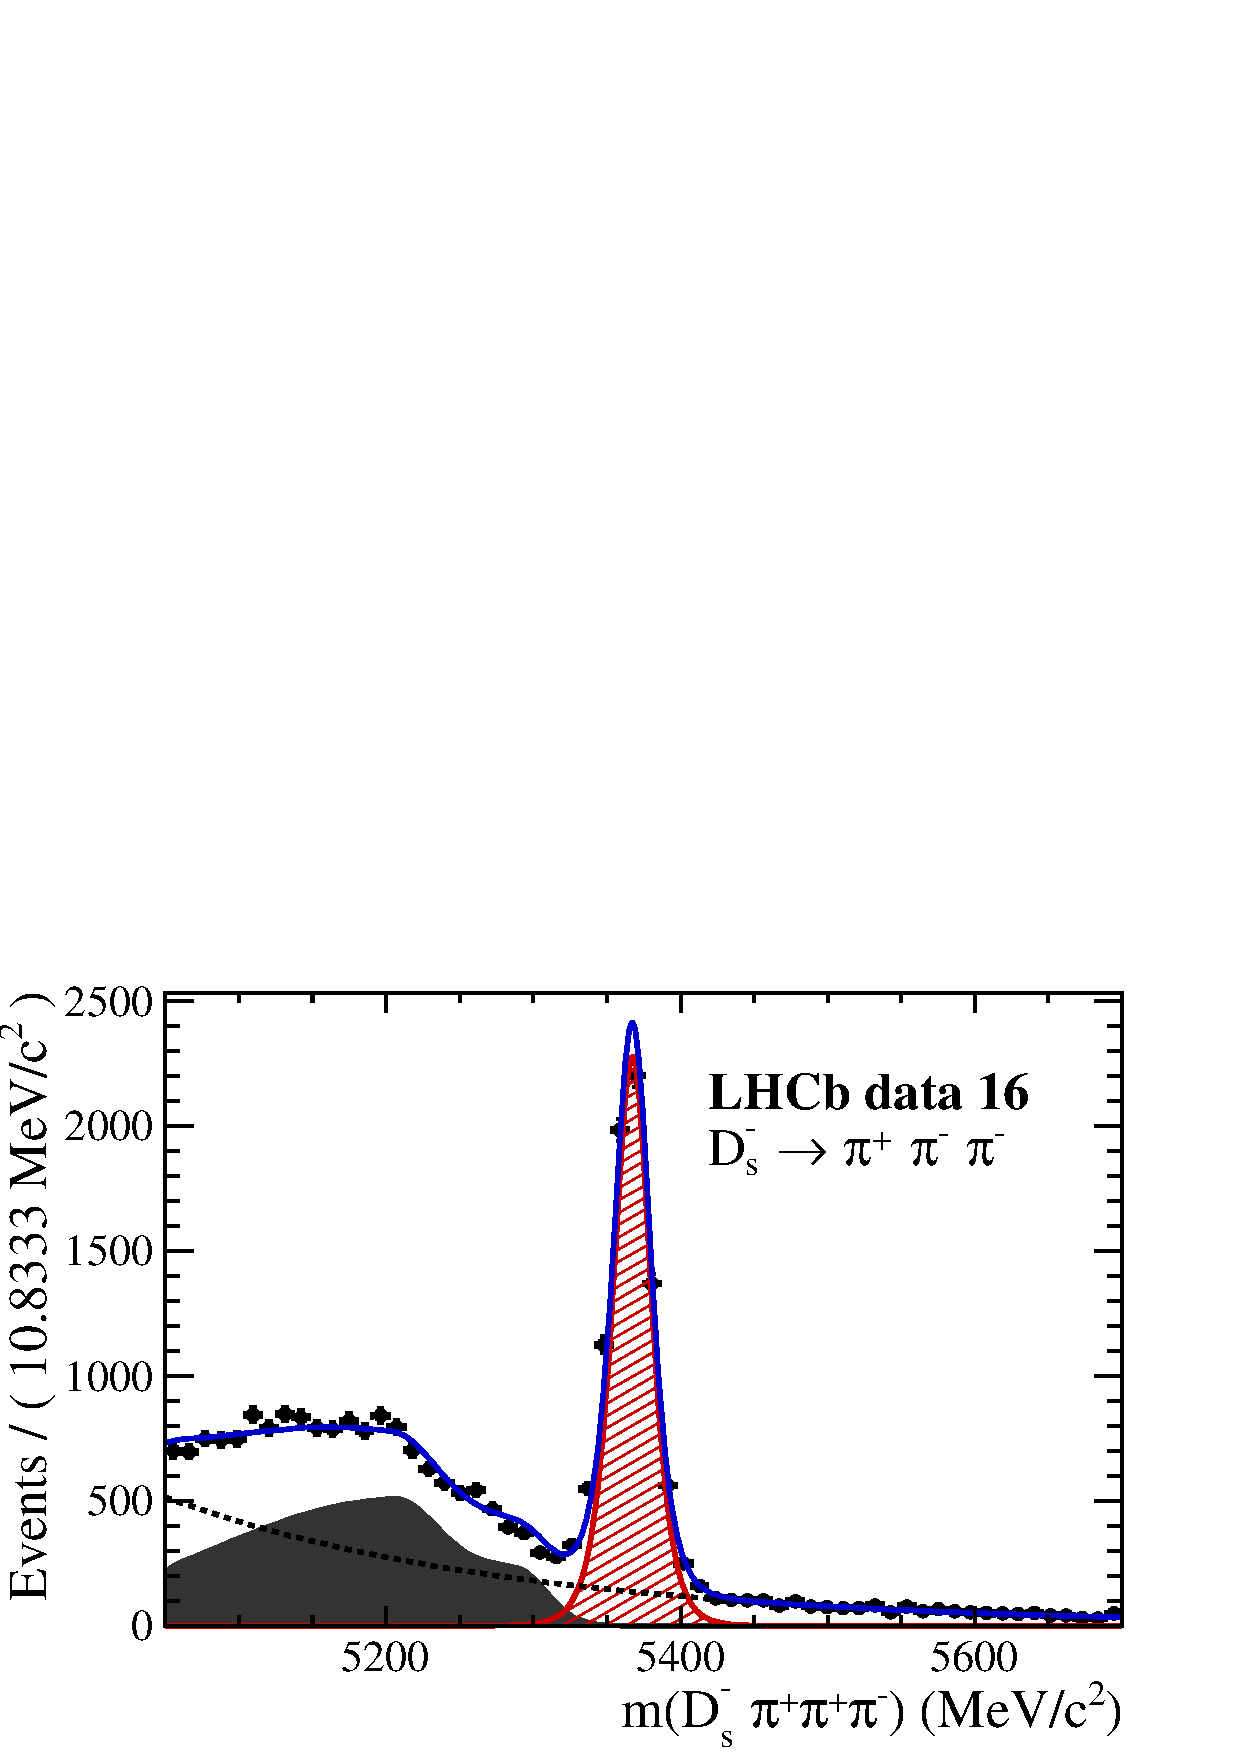
\includegraphics[height=!,width=0.5\textwidth]{figs/MassFit/norm_y16_pipipi.pdf}
\caption{Invariant mass distributions of $\Bs\to\Ds\pion\pion\pion$ candidates, ordered by $\Ds$ final state, for Run2 data.
The fit described in \ref{subsec: NormFit} is overlaid.}
\label{fig:massfits_norm_Run2}
\end{figure}

\clearpage

\begin{figure}[h]
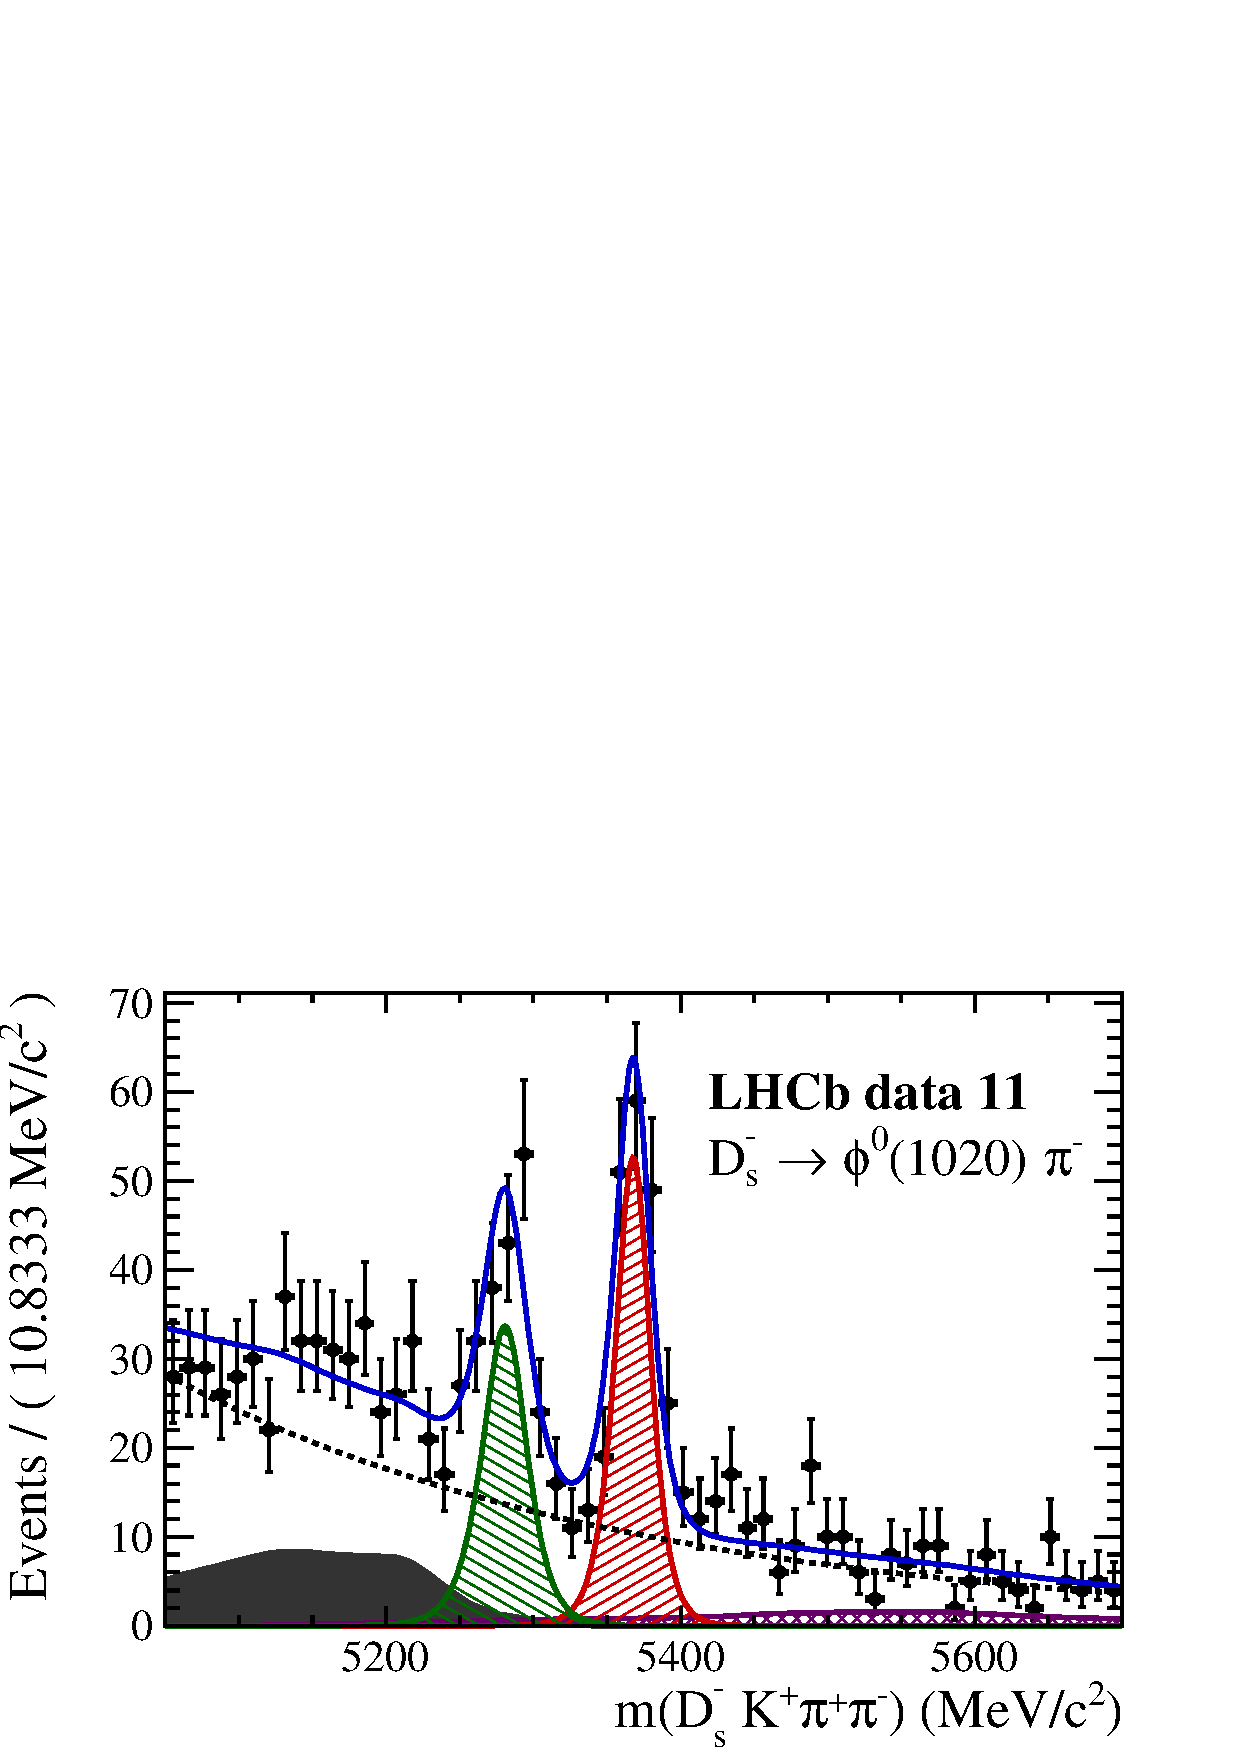
\includegraphics[height=!,width=0.5\textwidth]{figs/MassFit/signal_y11_phipi.pdf}
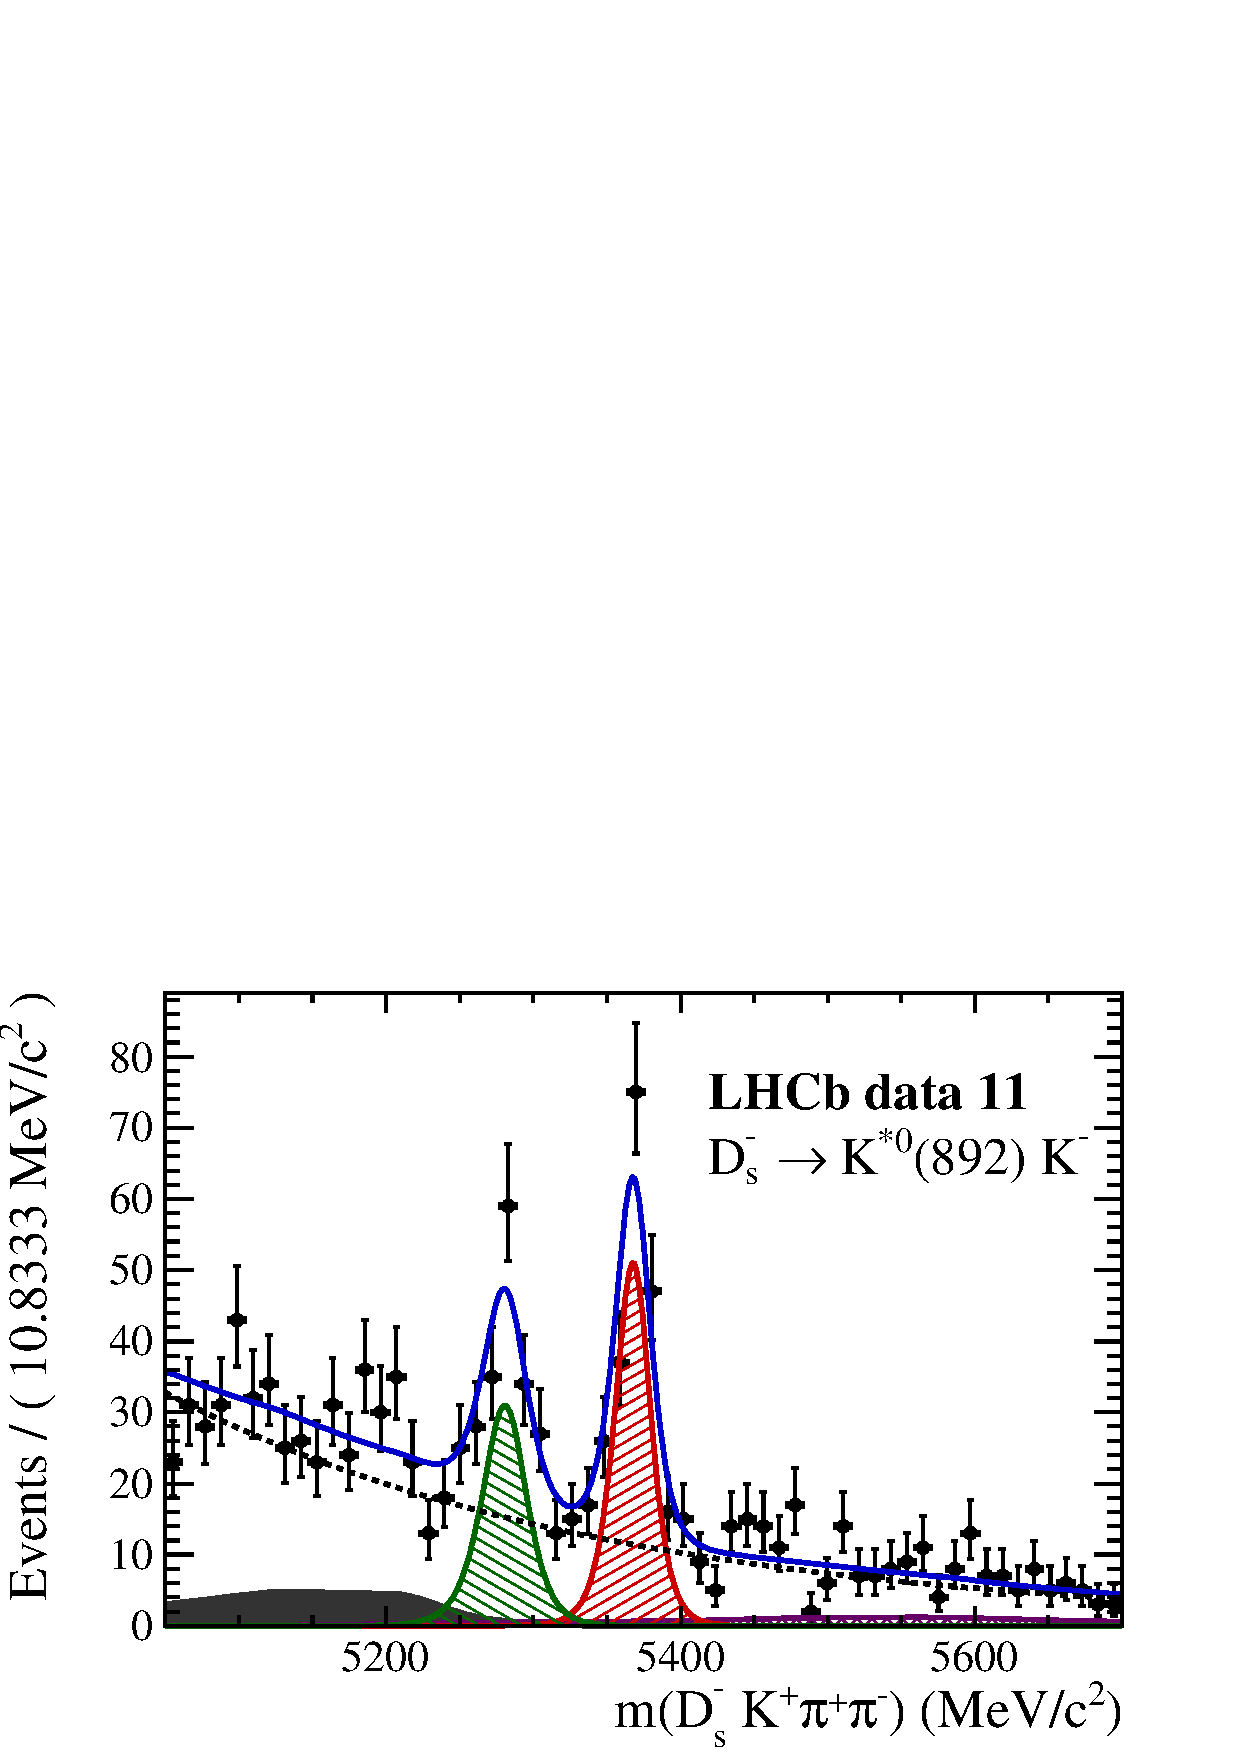
\includegraphics[height=!,width=0.5\textwidth]{figs/MassFit/signal_y11_KsK.pdf}
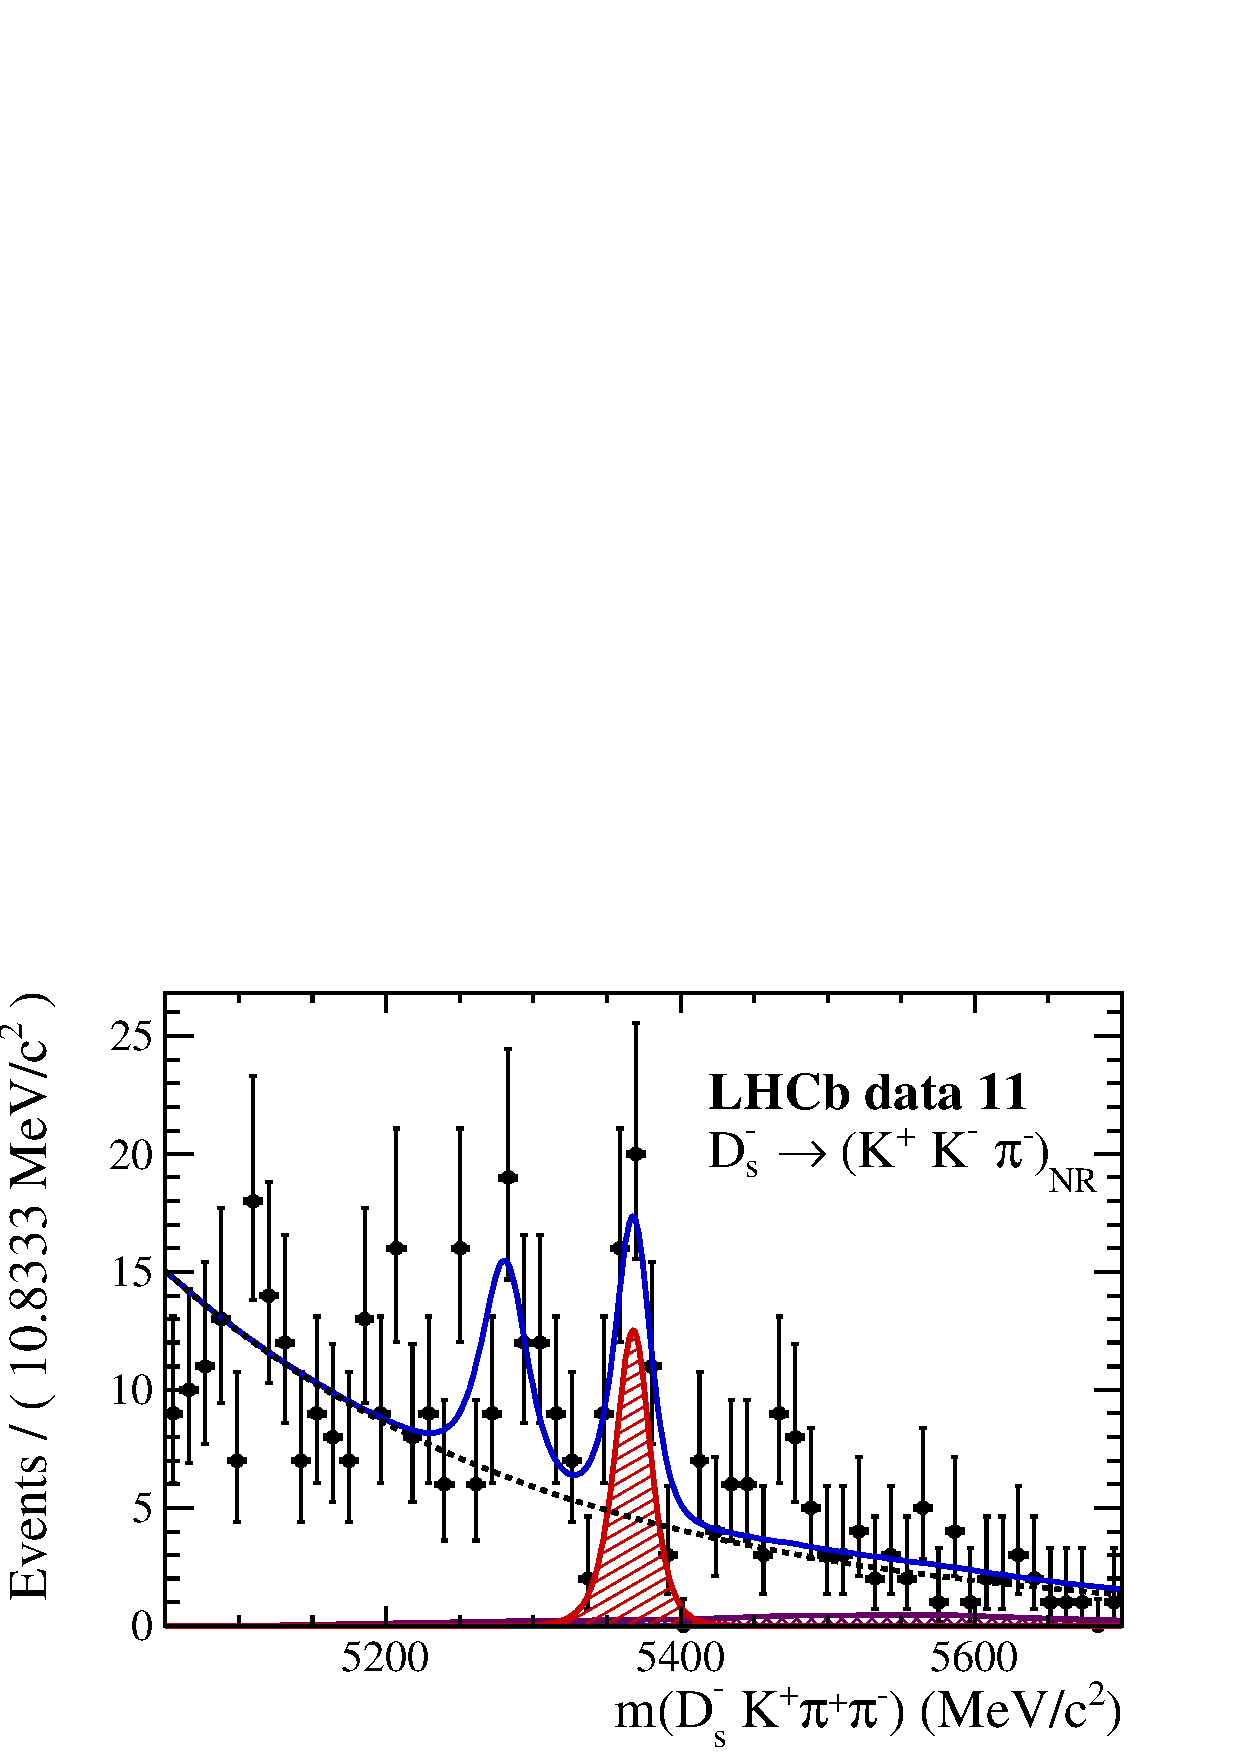
\includegraphics[height=!,width=0.5\textwidth]{figs/MassFit/signal_y11_KKpi_NR.pdf}
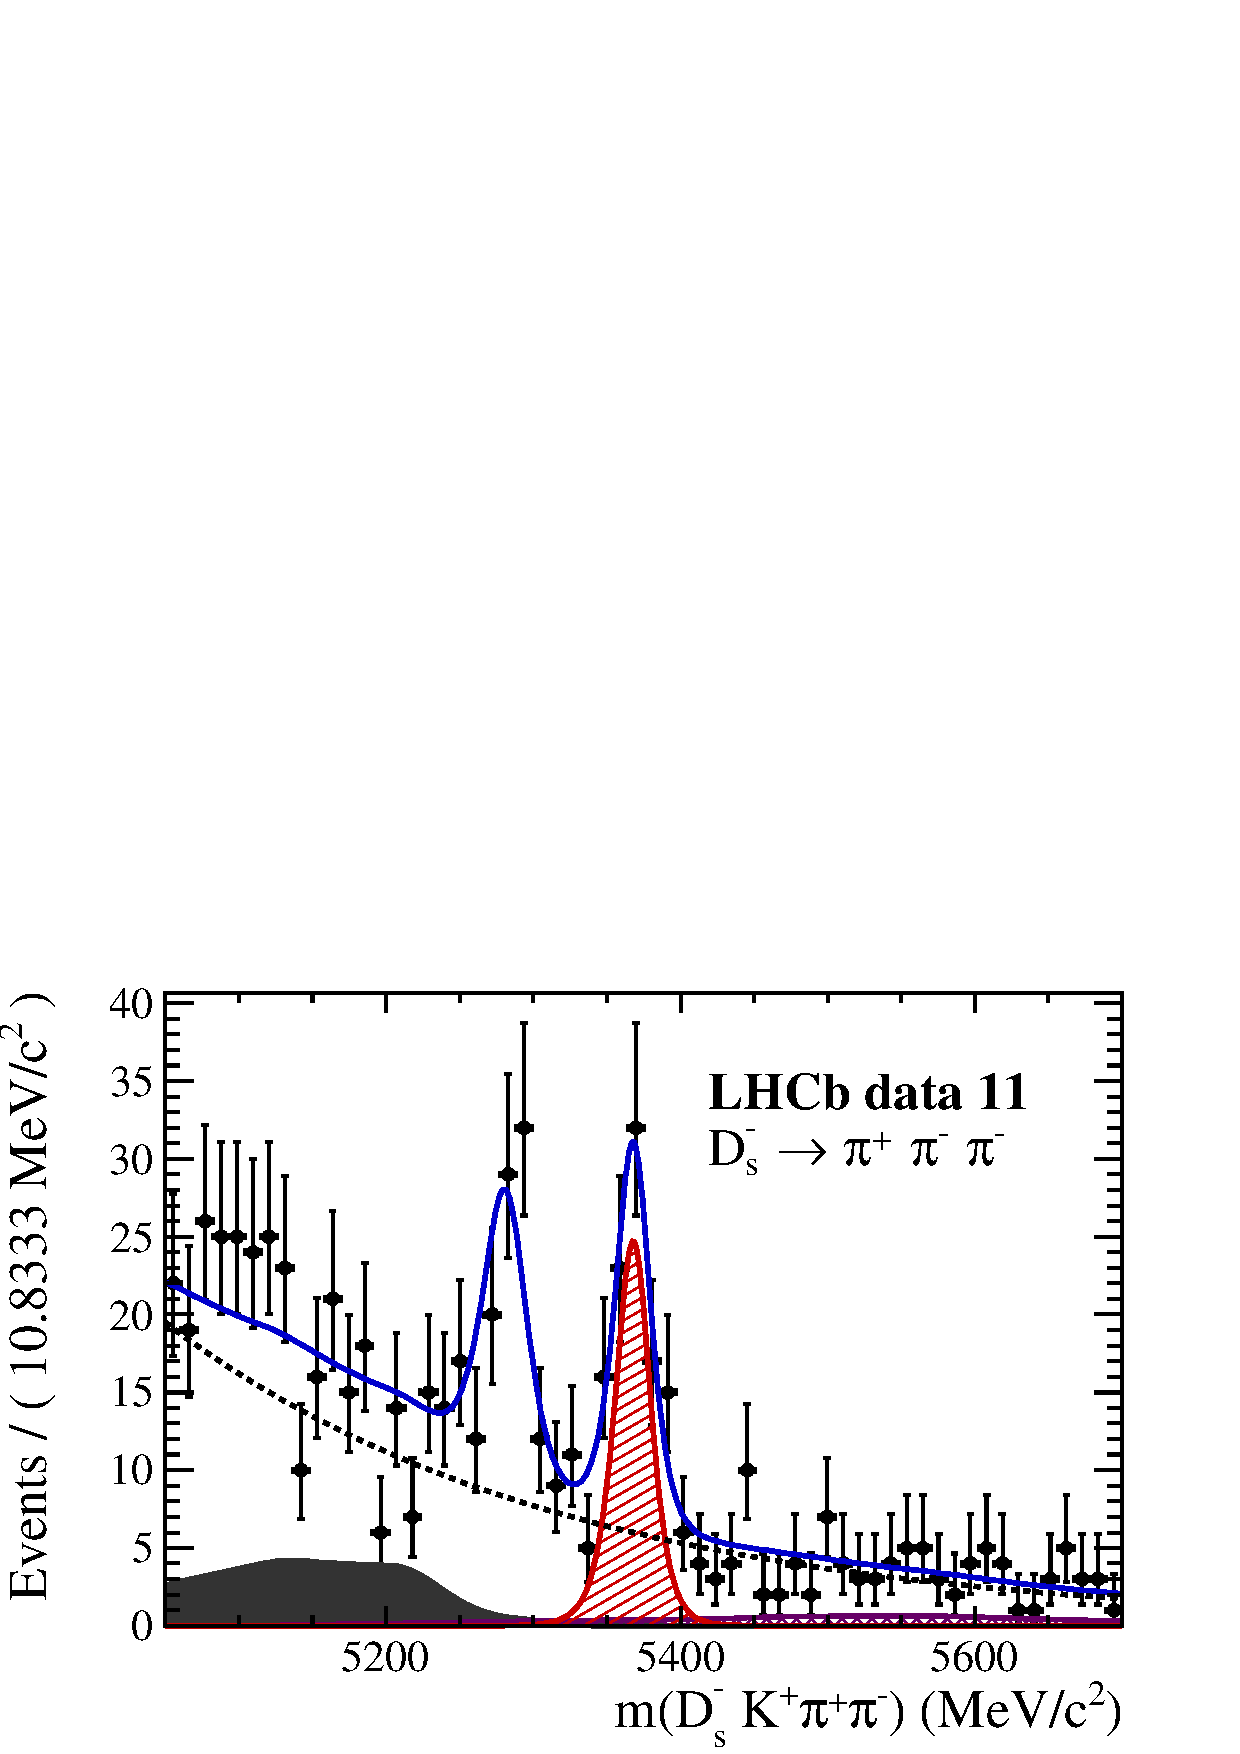
\includegraphics[height=!,width=0.5\textwidth]{figs/MassFit/signal_y11_pipipi.pdf}
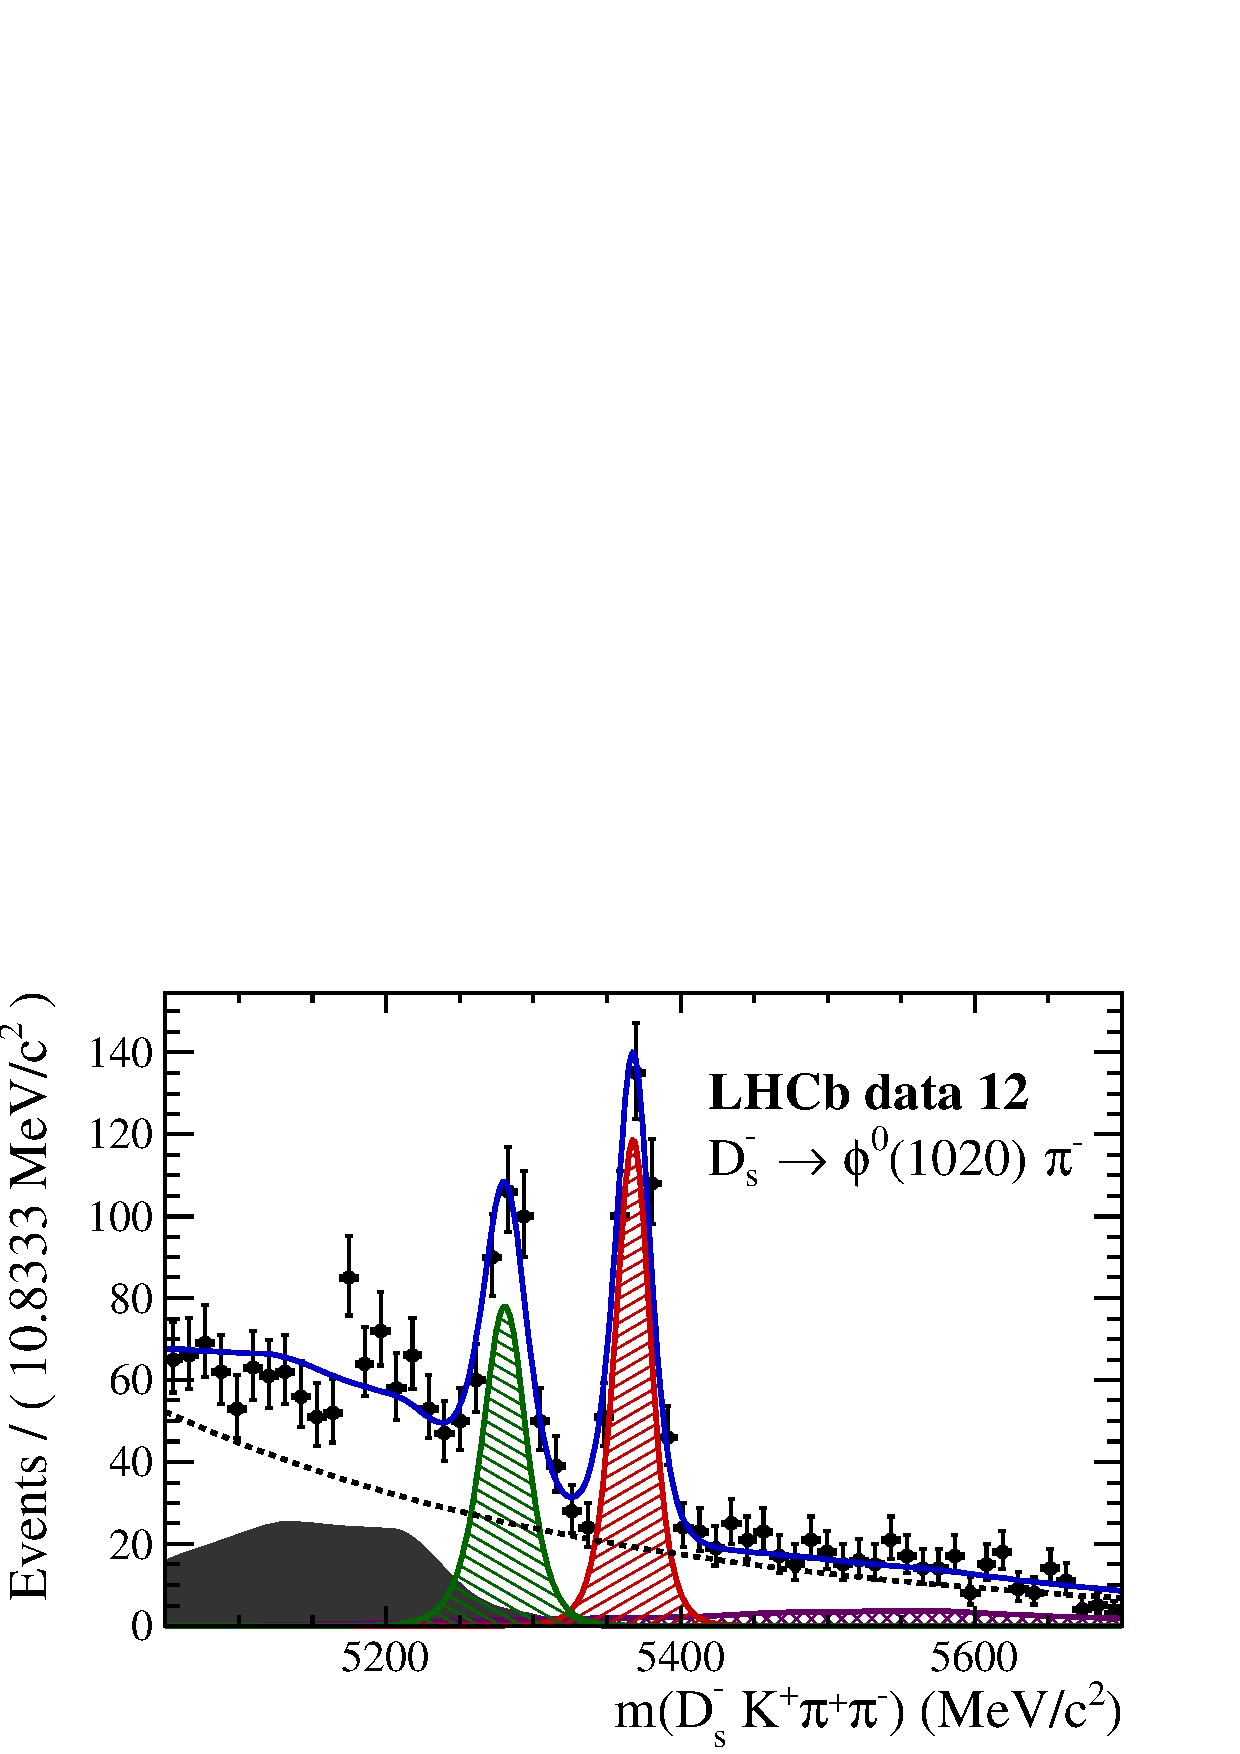
\includegraphics[height=!,width=0.5\textwidth]{figs/MassFit/signal_y12_phipi.pdf}
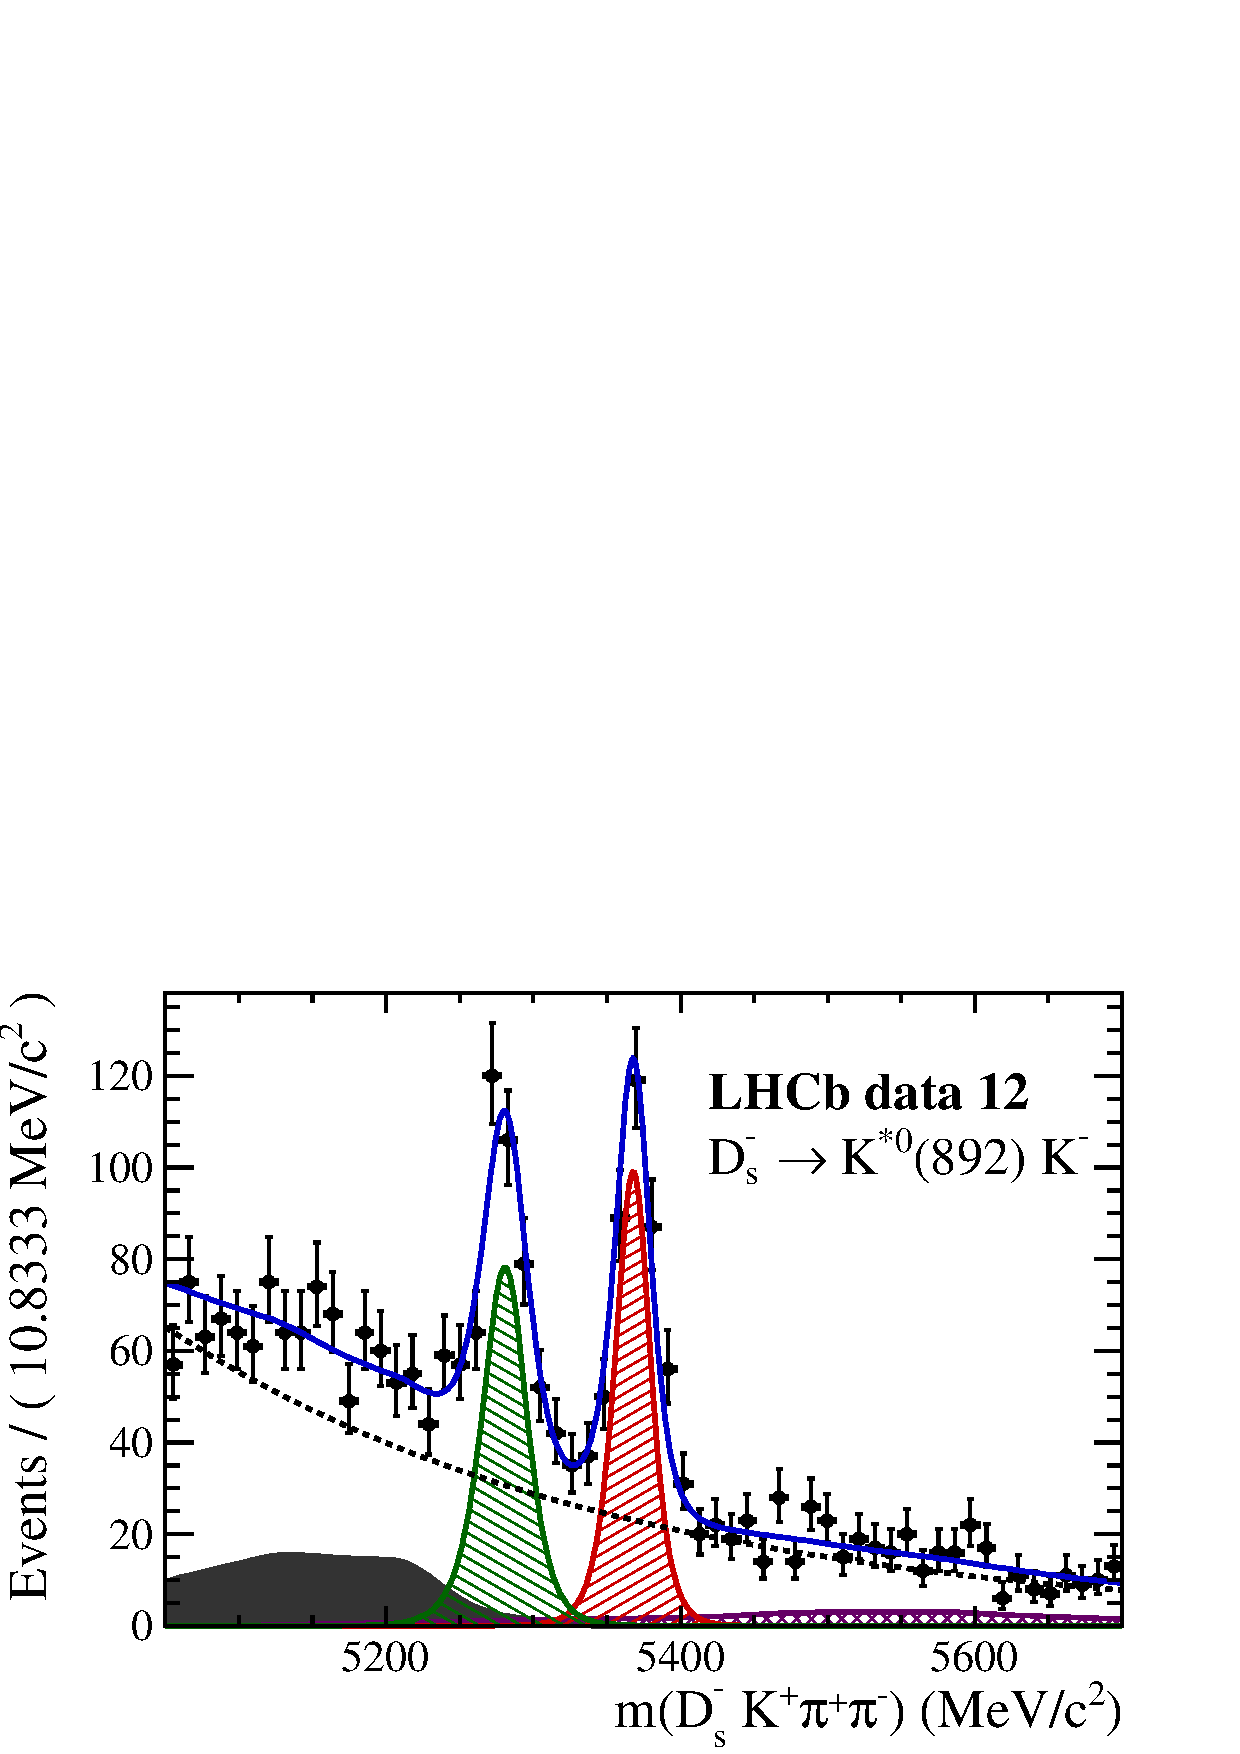
\includegraphics[height=!,width=0.5\textwidth]{figs/MassFit/signal_y12_KsK.pdf}
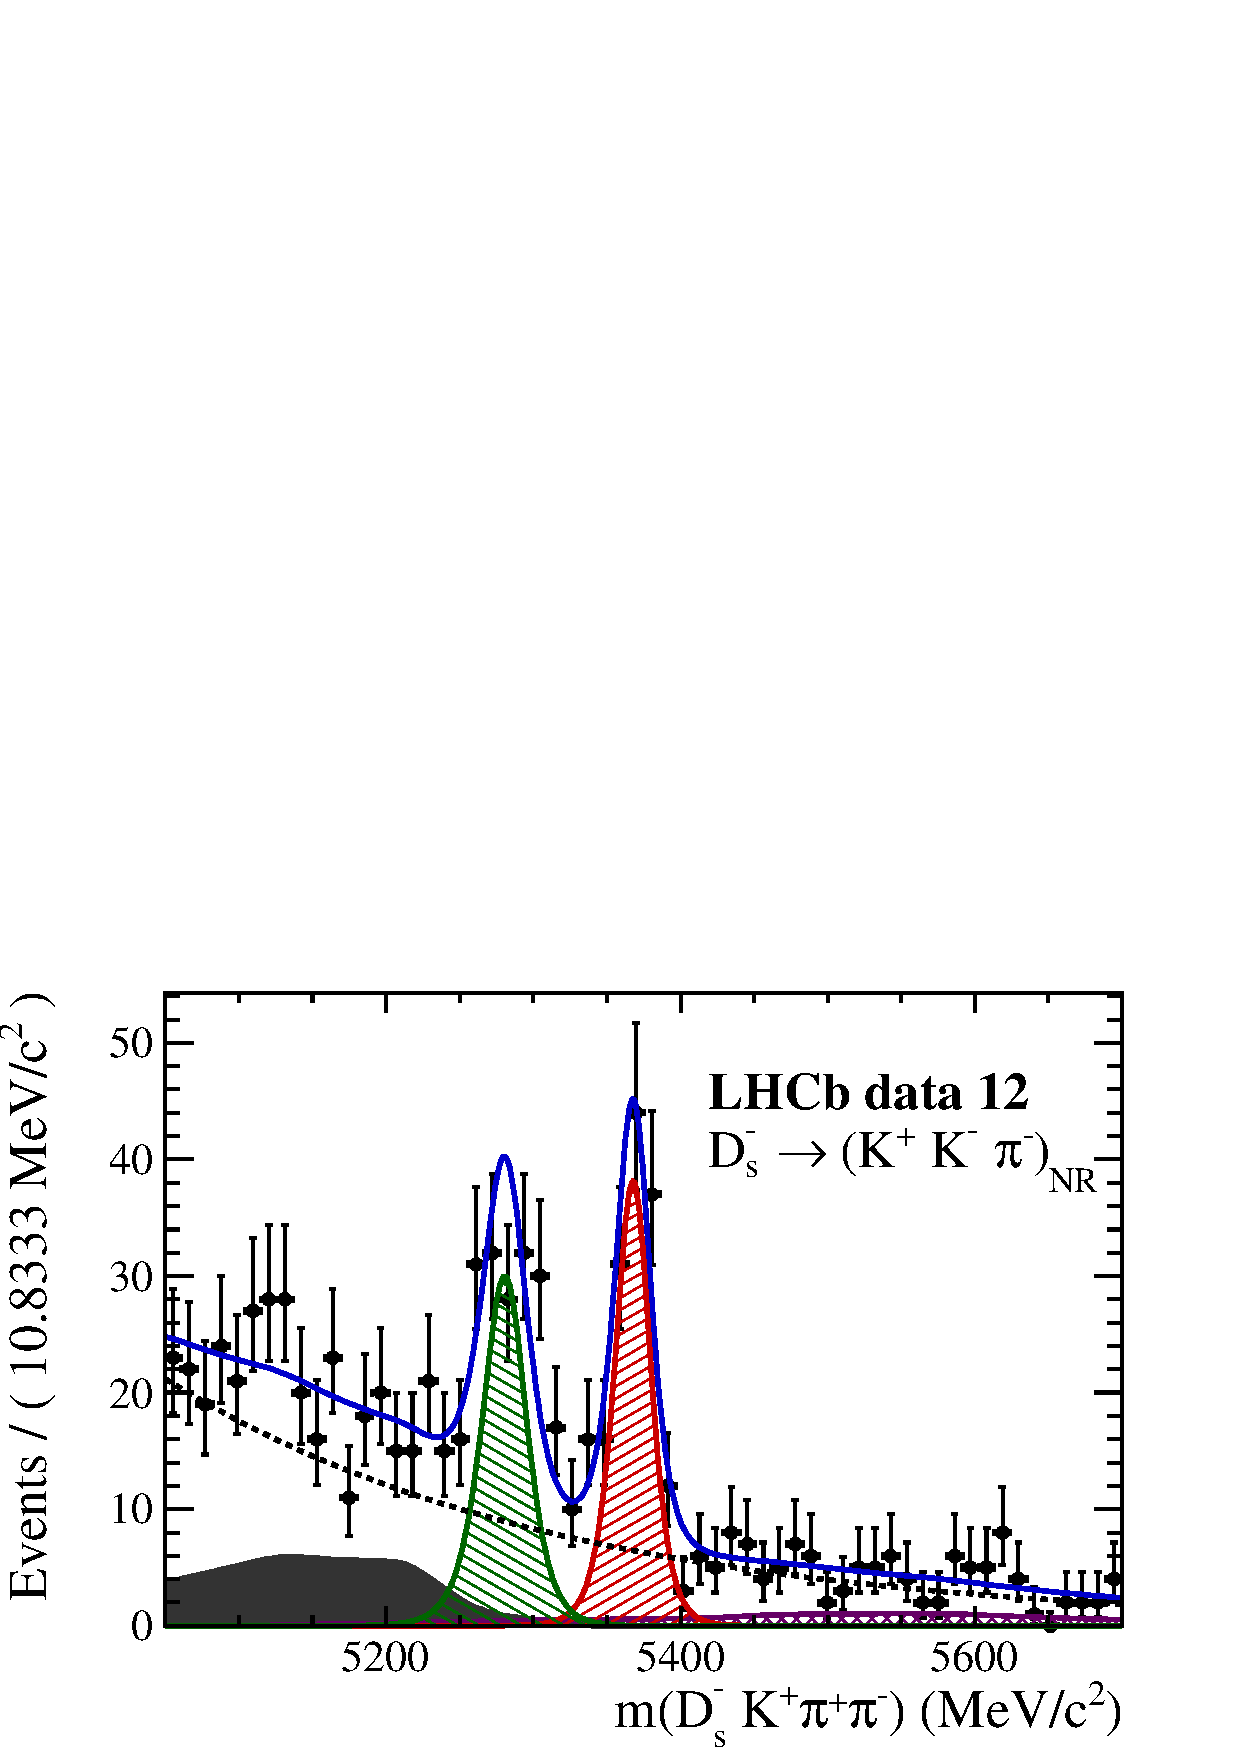
\includegraphics[height=!,width=0.5\textwidth]{figs/MassFit/signal_y12_KKpi_NR.pdf}
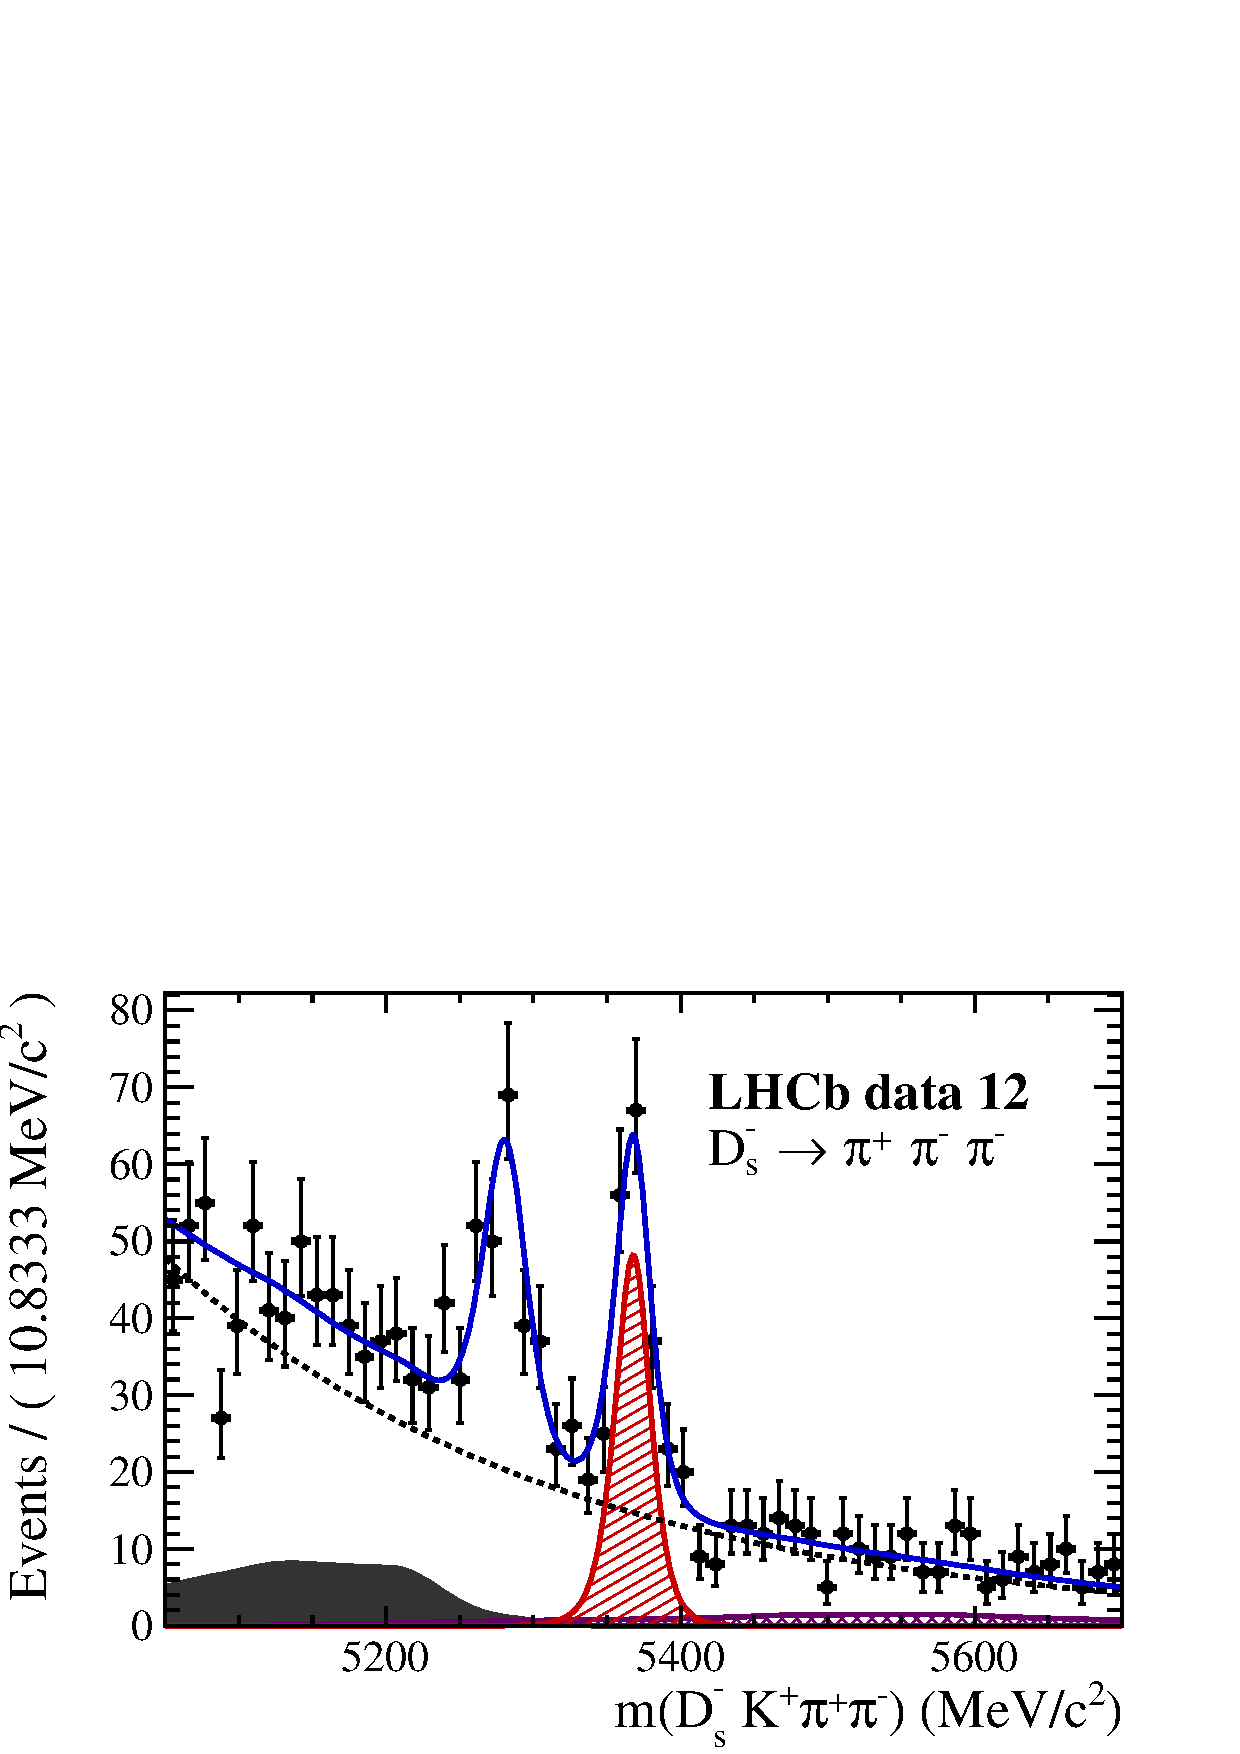
\includegraphics[height=!,width=0.5\textwidth]{figs/MassFit/signal_y12_pipipi.pdf}
\caption{Invariant mass distributions of $\Bs\to\Ds\kaon\pion\pion$ candidates, ordered by $\Ds$ final state, for Run1 data.
The fit described in \ref{subsec: SigFit} is overlaid.}
\label{fig:massfits_signal_Run1}
\end{figure}

\clearpage

\begin{figure}[h]
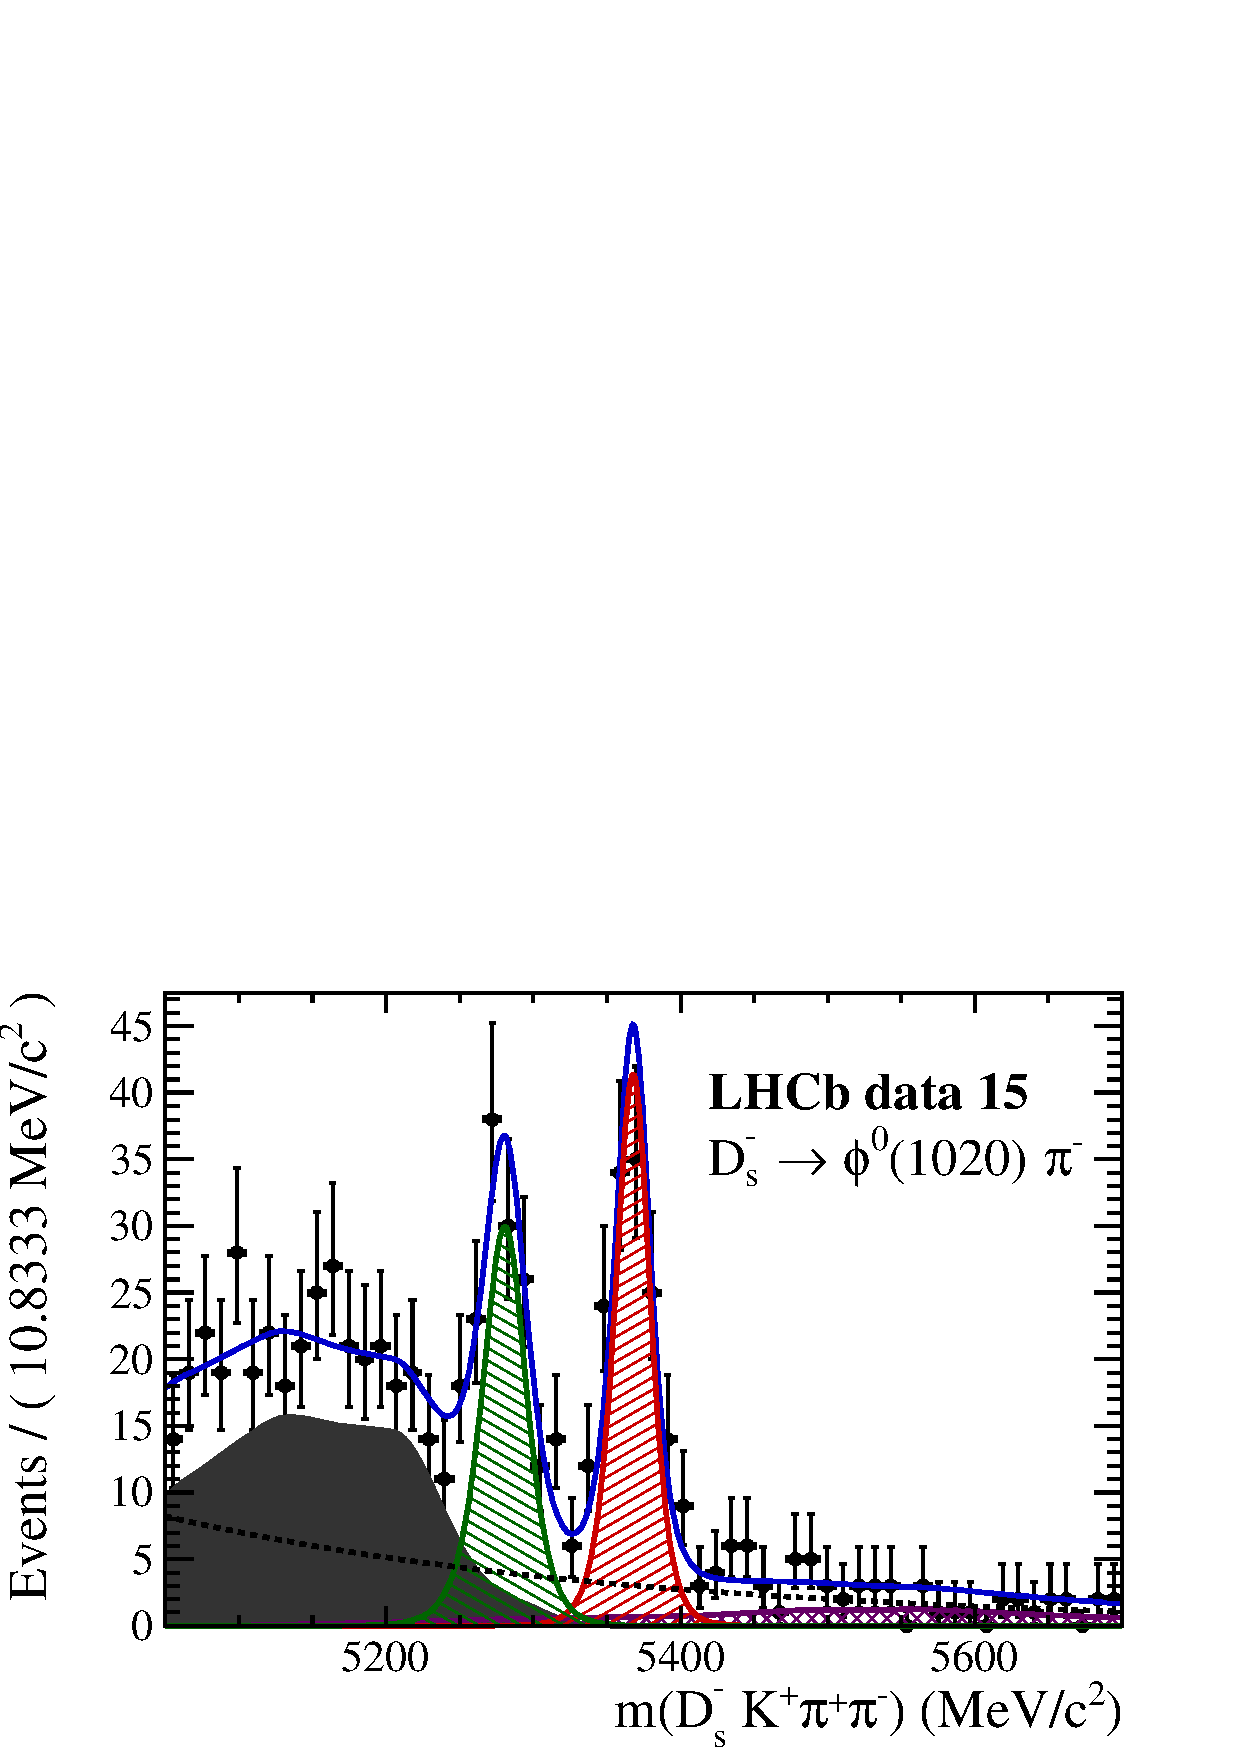
\includegraphics[height=!,width=0.5\textwidth]{figs/MassFit/signal_y15_phipi.pdf}
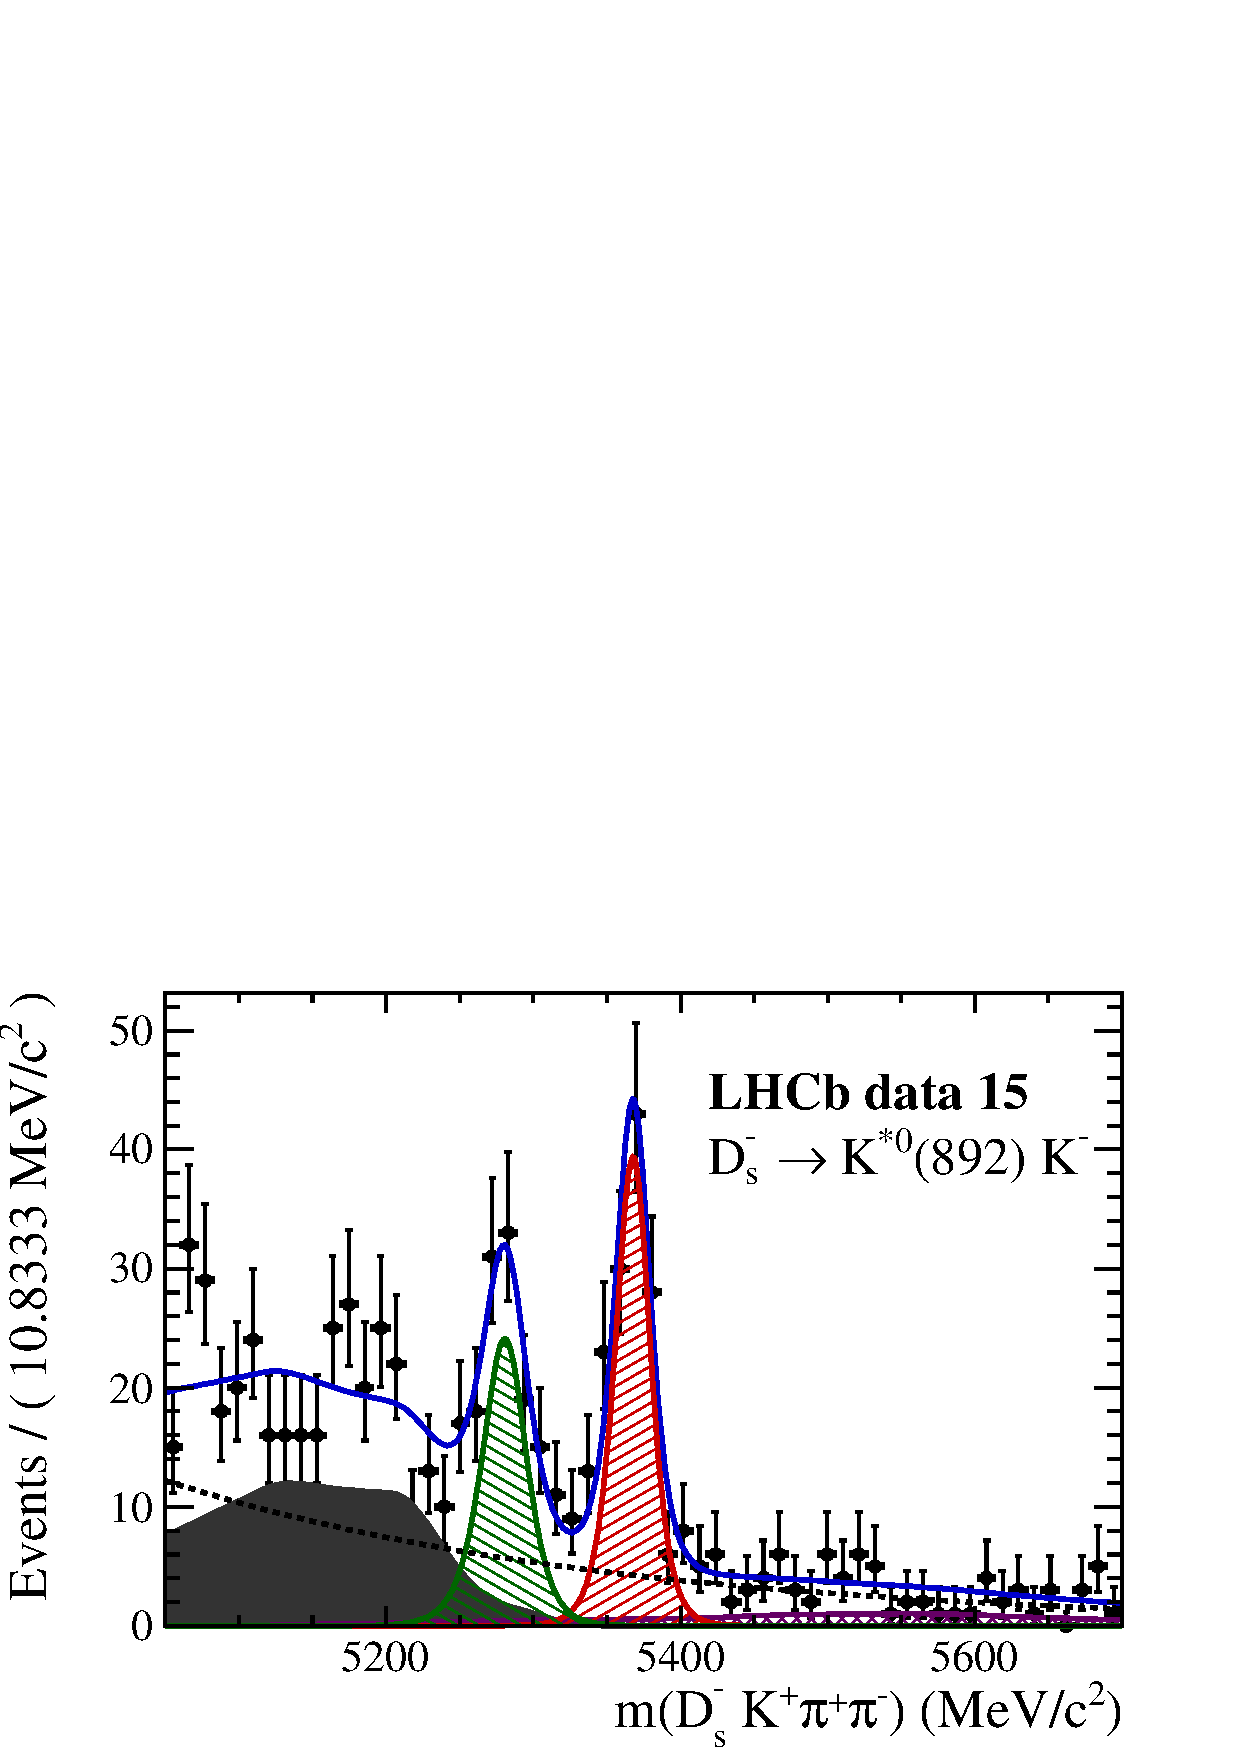
\includegraphics[height=!,width=0.5\textwidth]{figs/MassFit/signal_y15_KsK.pdf}
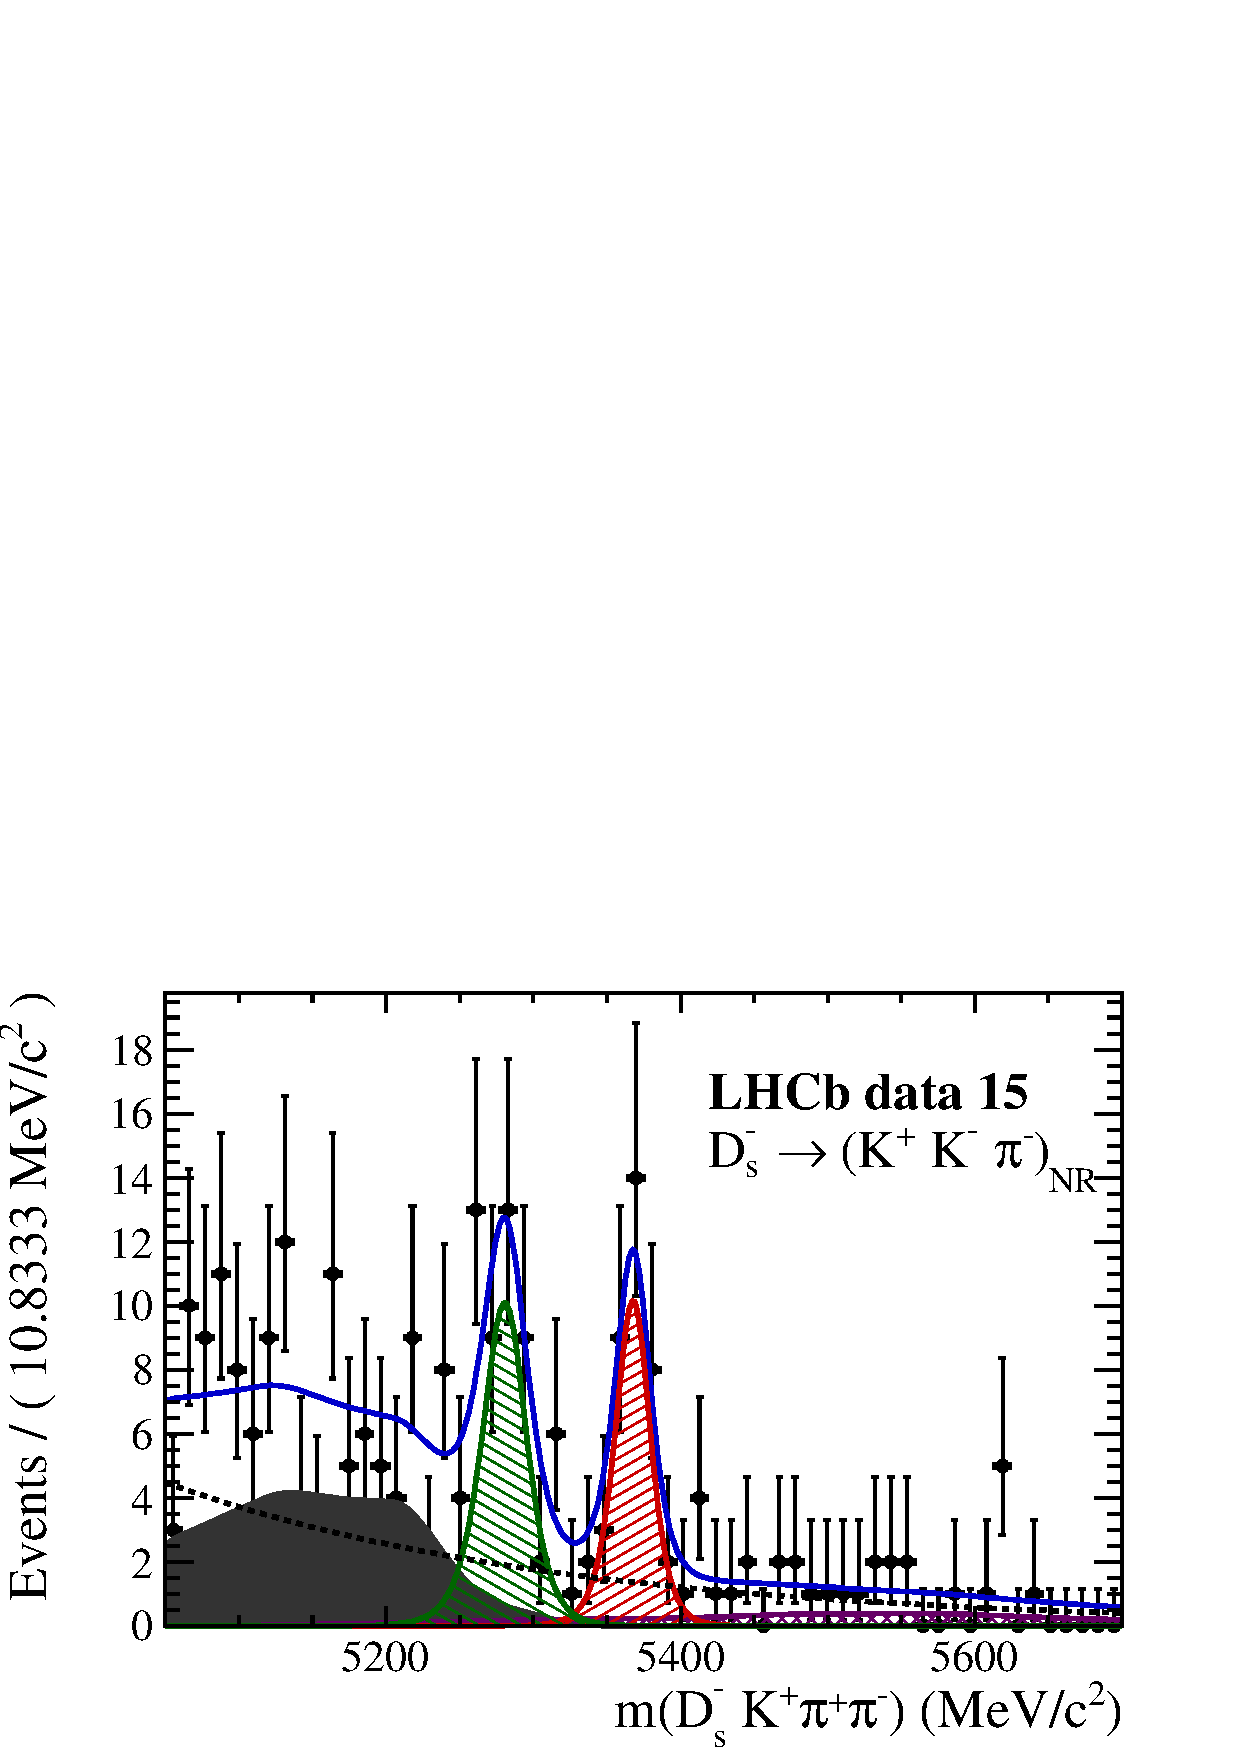
\includegraphics[height=!,width=0.5\textwidth]{figs/MassFit/signal_y15_KKpi_NR.pdf}
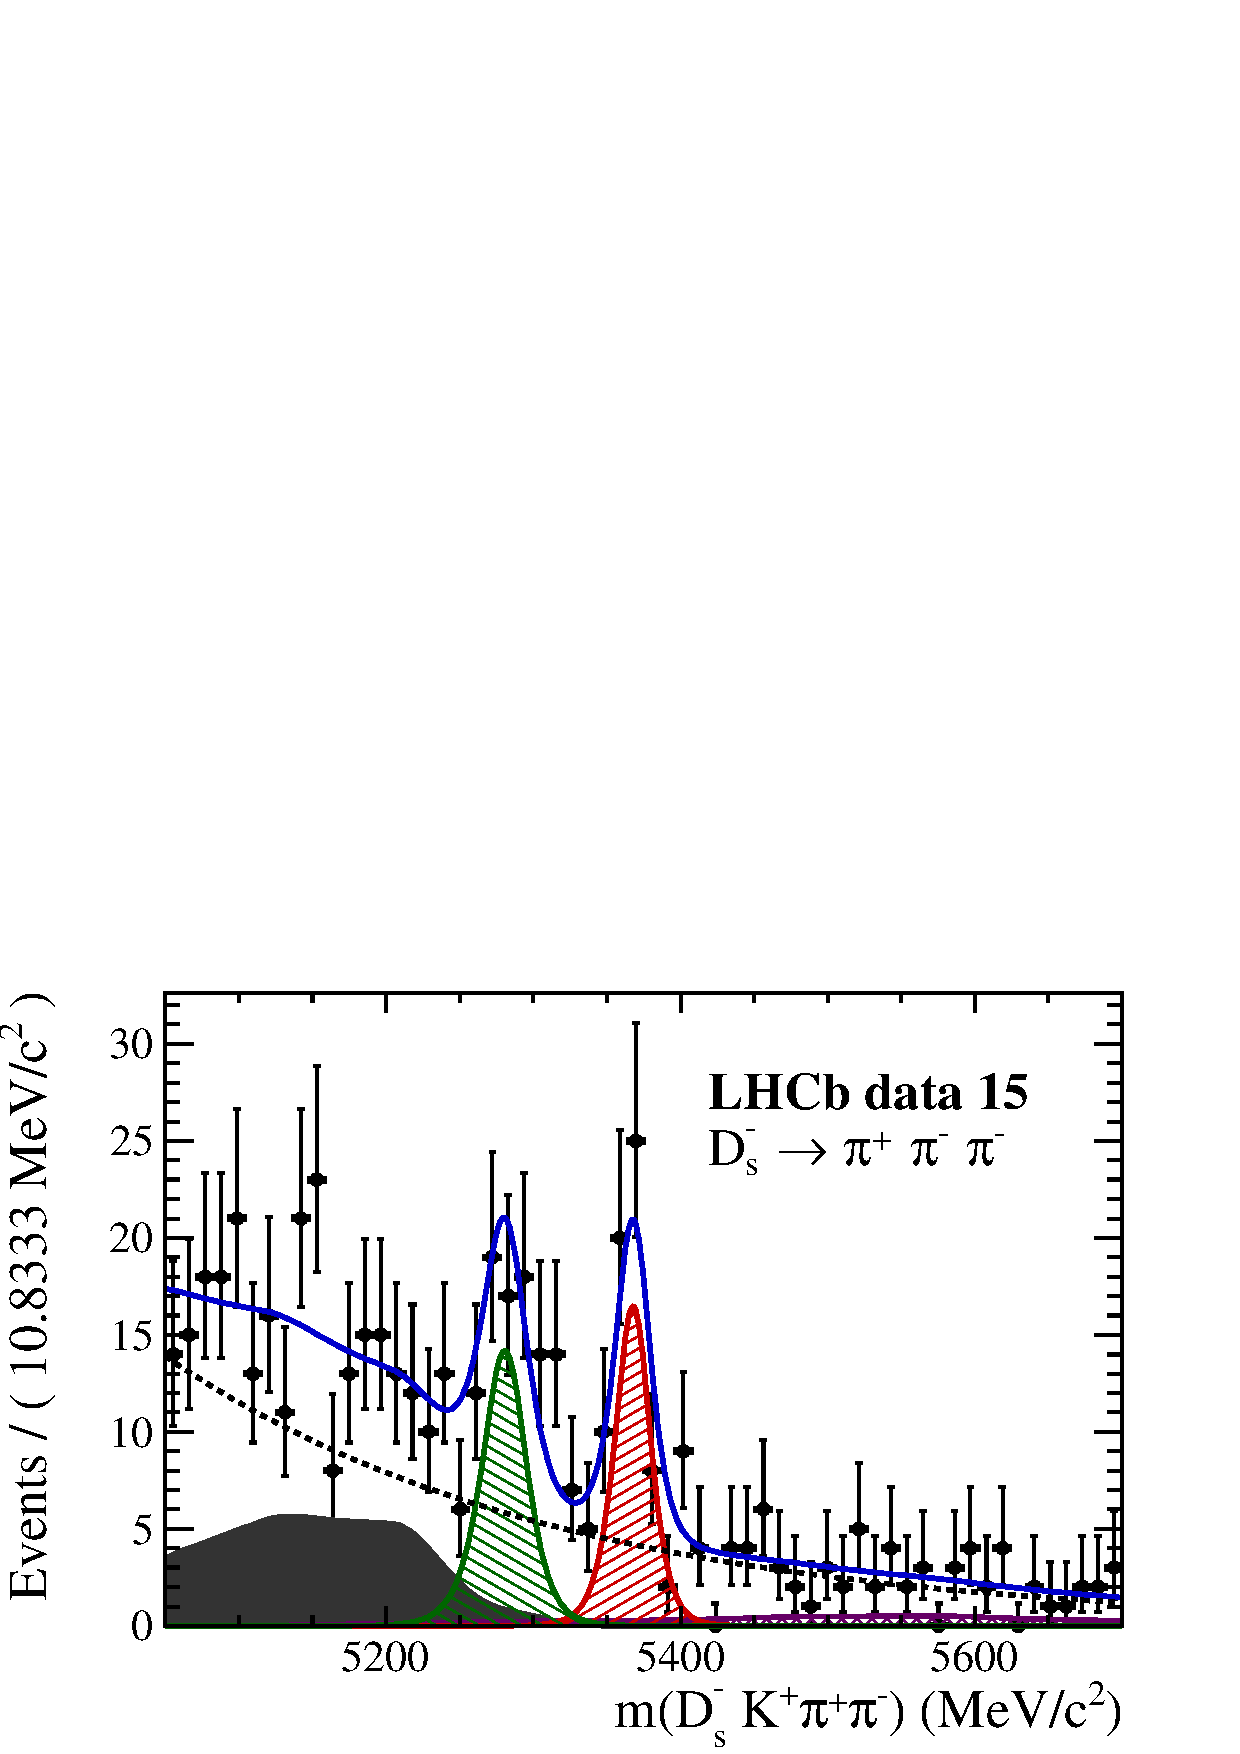
\includegraphics[height=!,width=0.5\textwidth]{figs/MassFit/signal_y15_pipipi.pdf}
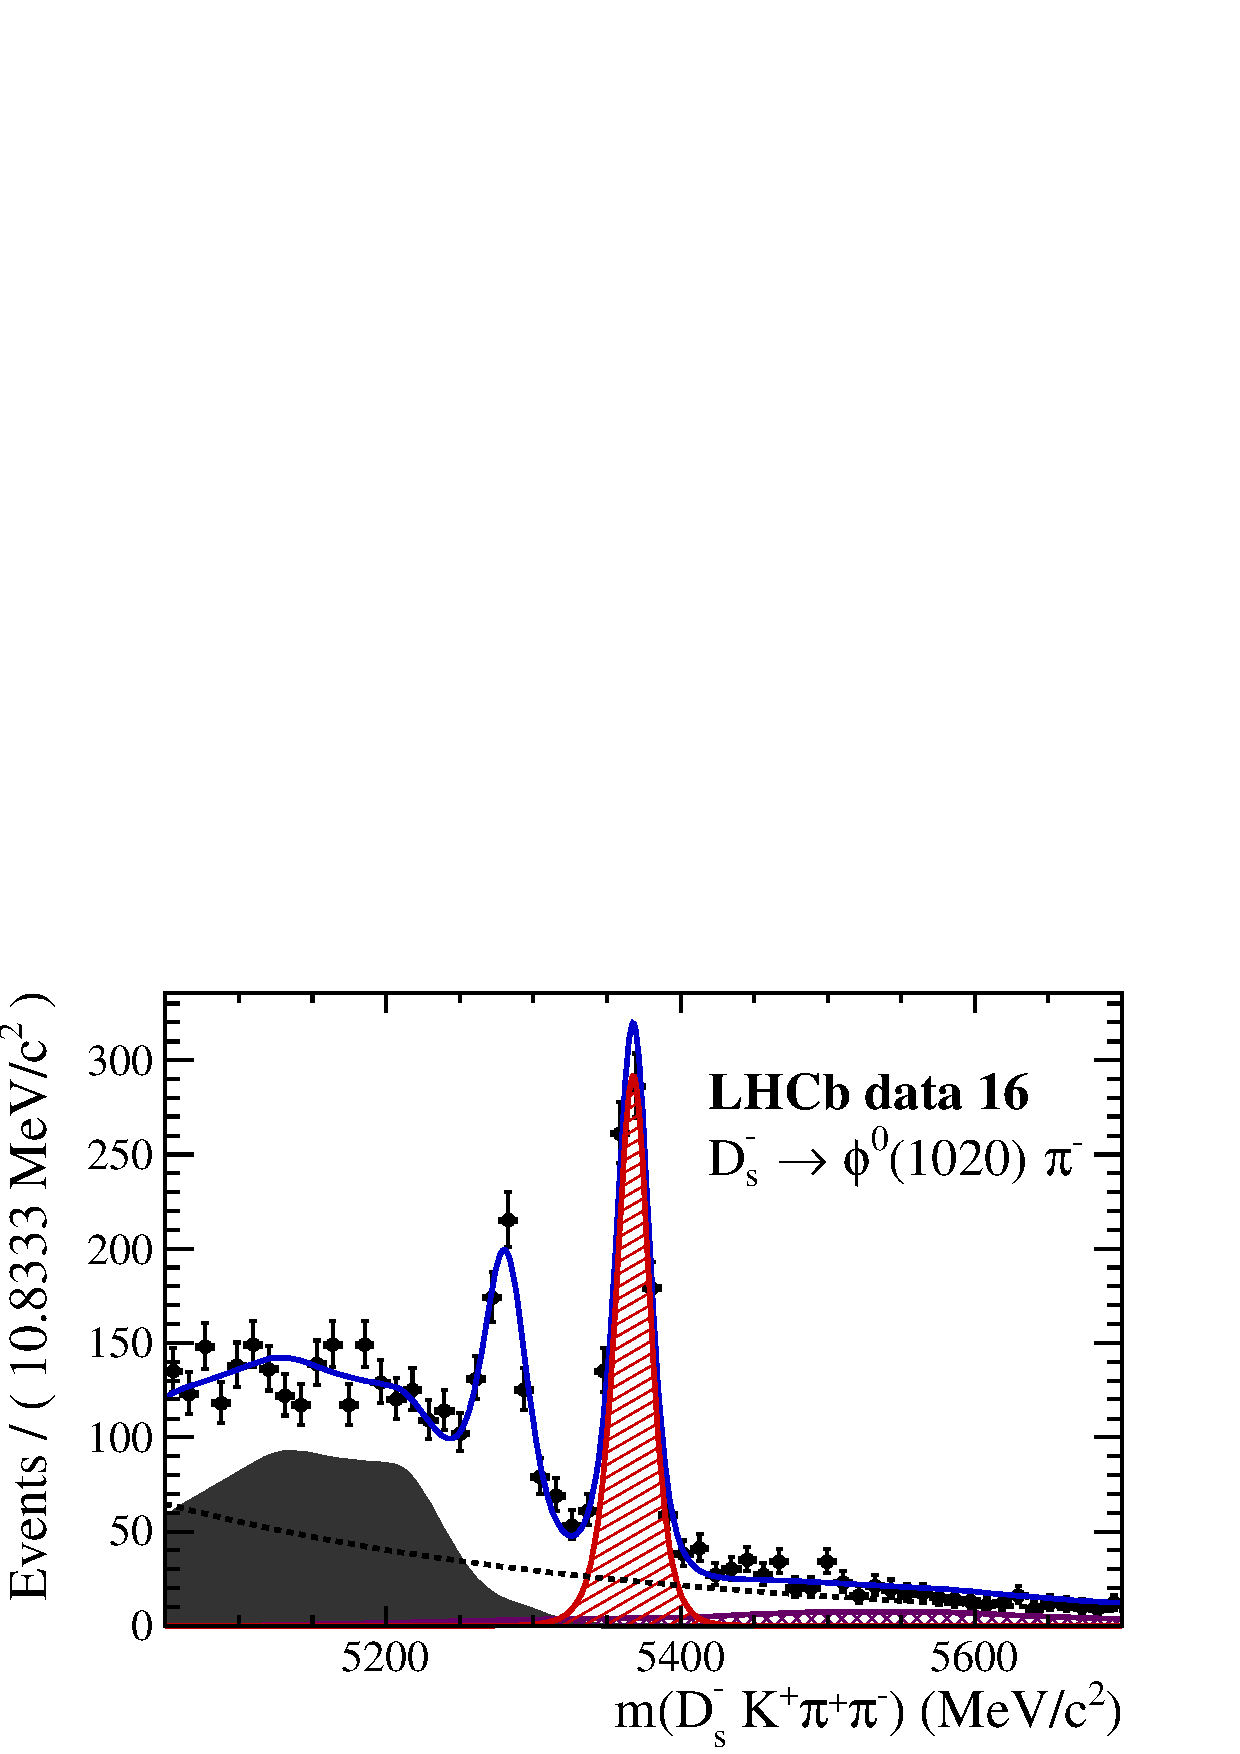
\includegraphics[height=!,width=0.5\textwidth]{figs/MassFit/signal_y16_phipi.pdf}
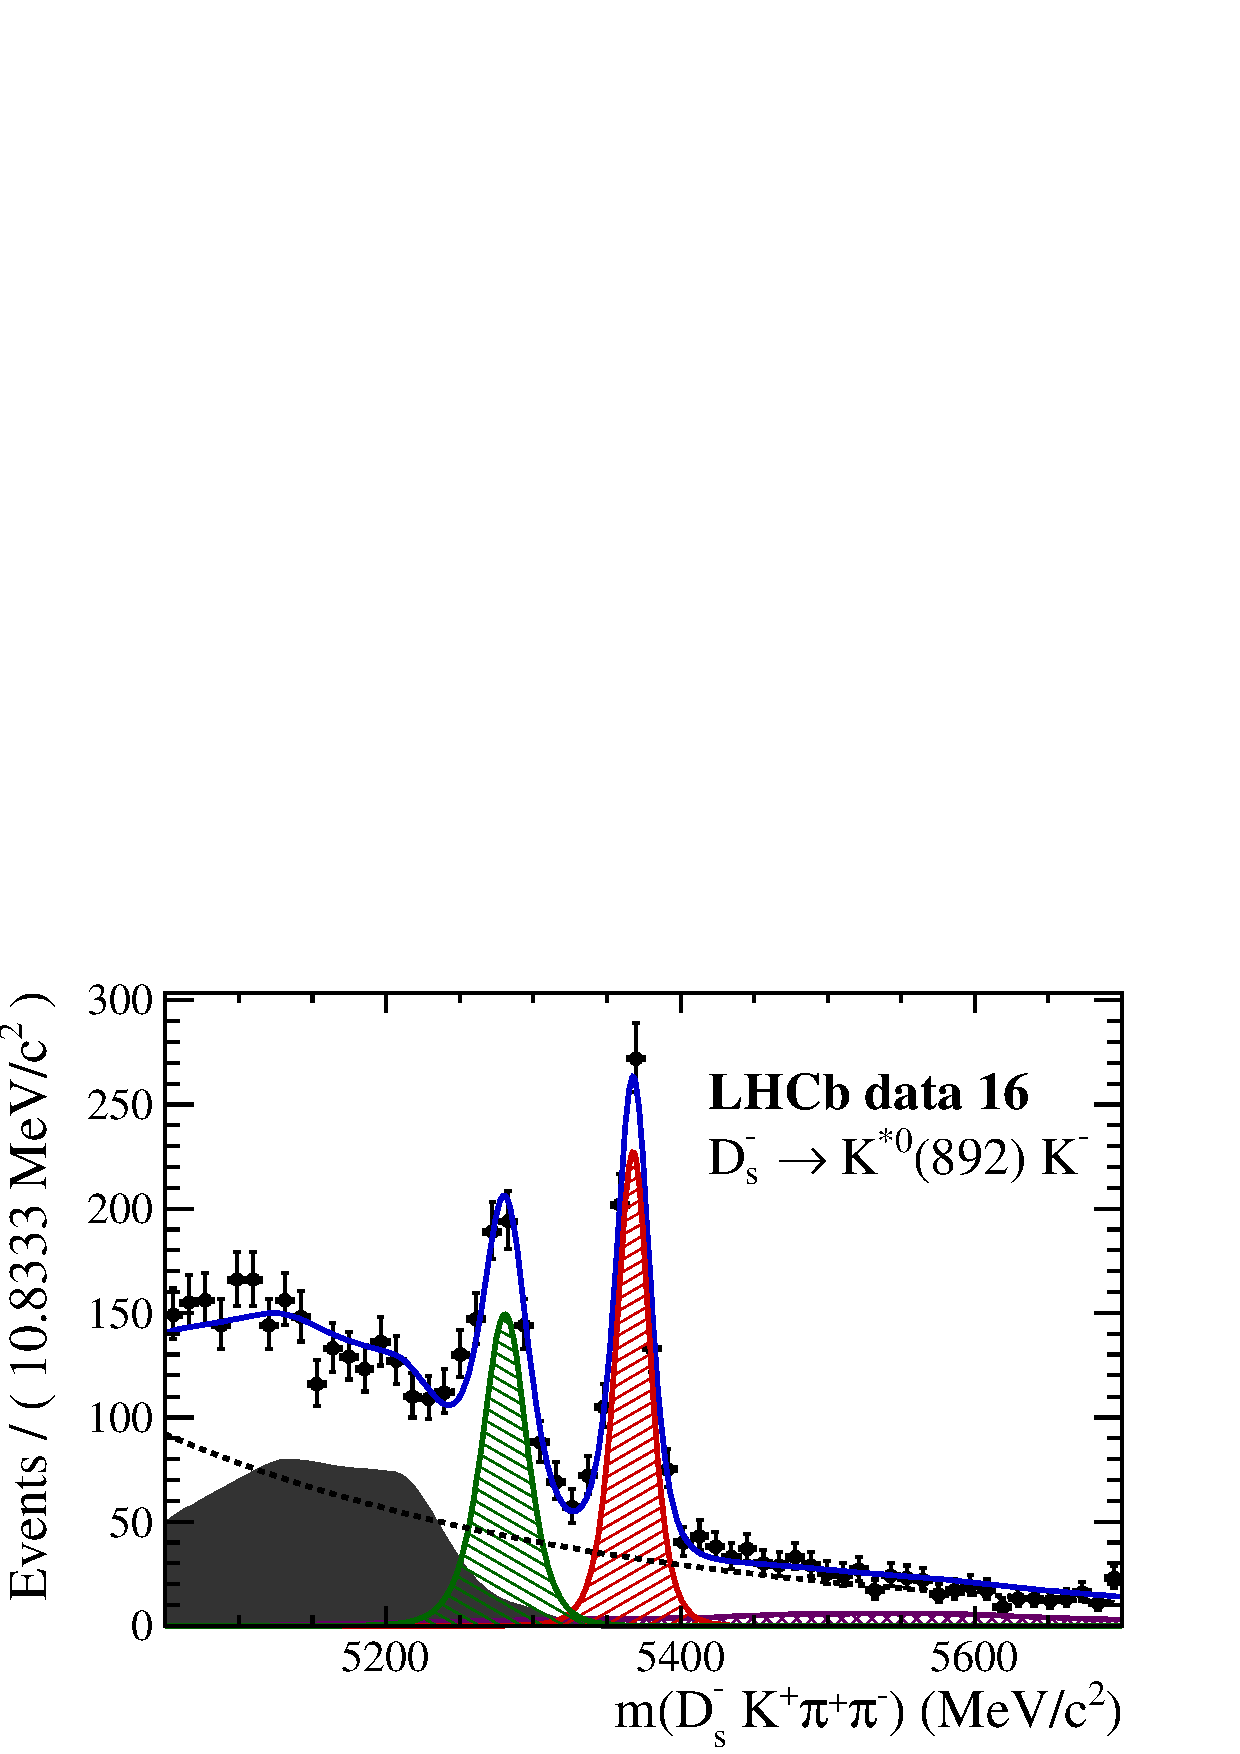
\includegraphics[height=!,width=0.5\textwidth]{figs/MassFit/signal_y16_KsK.pdf}
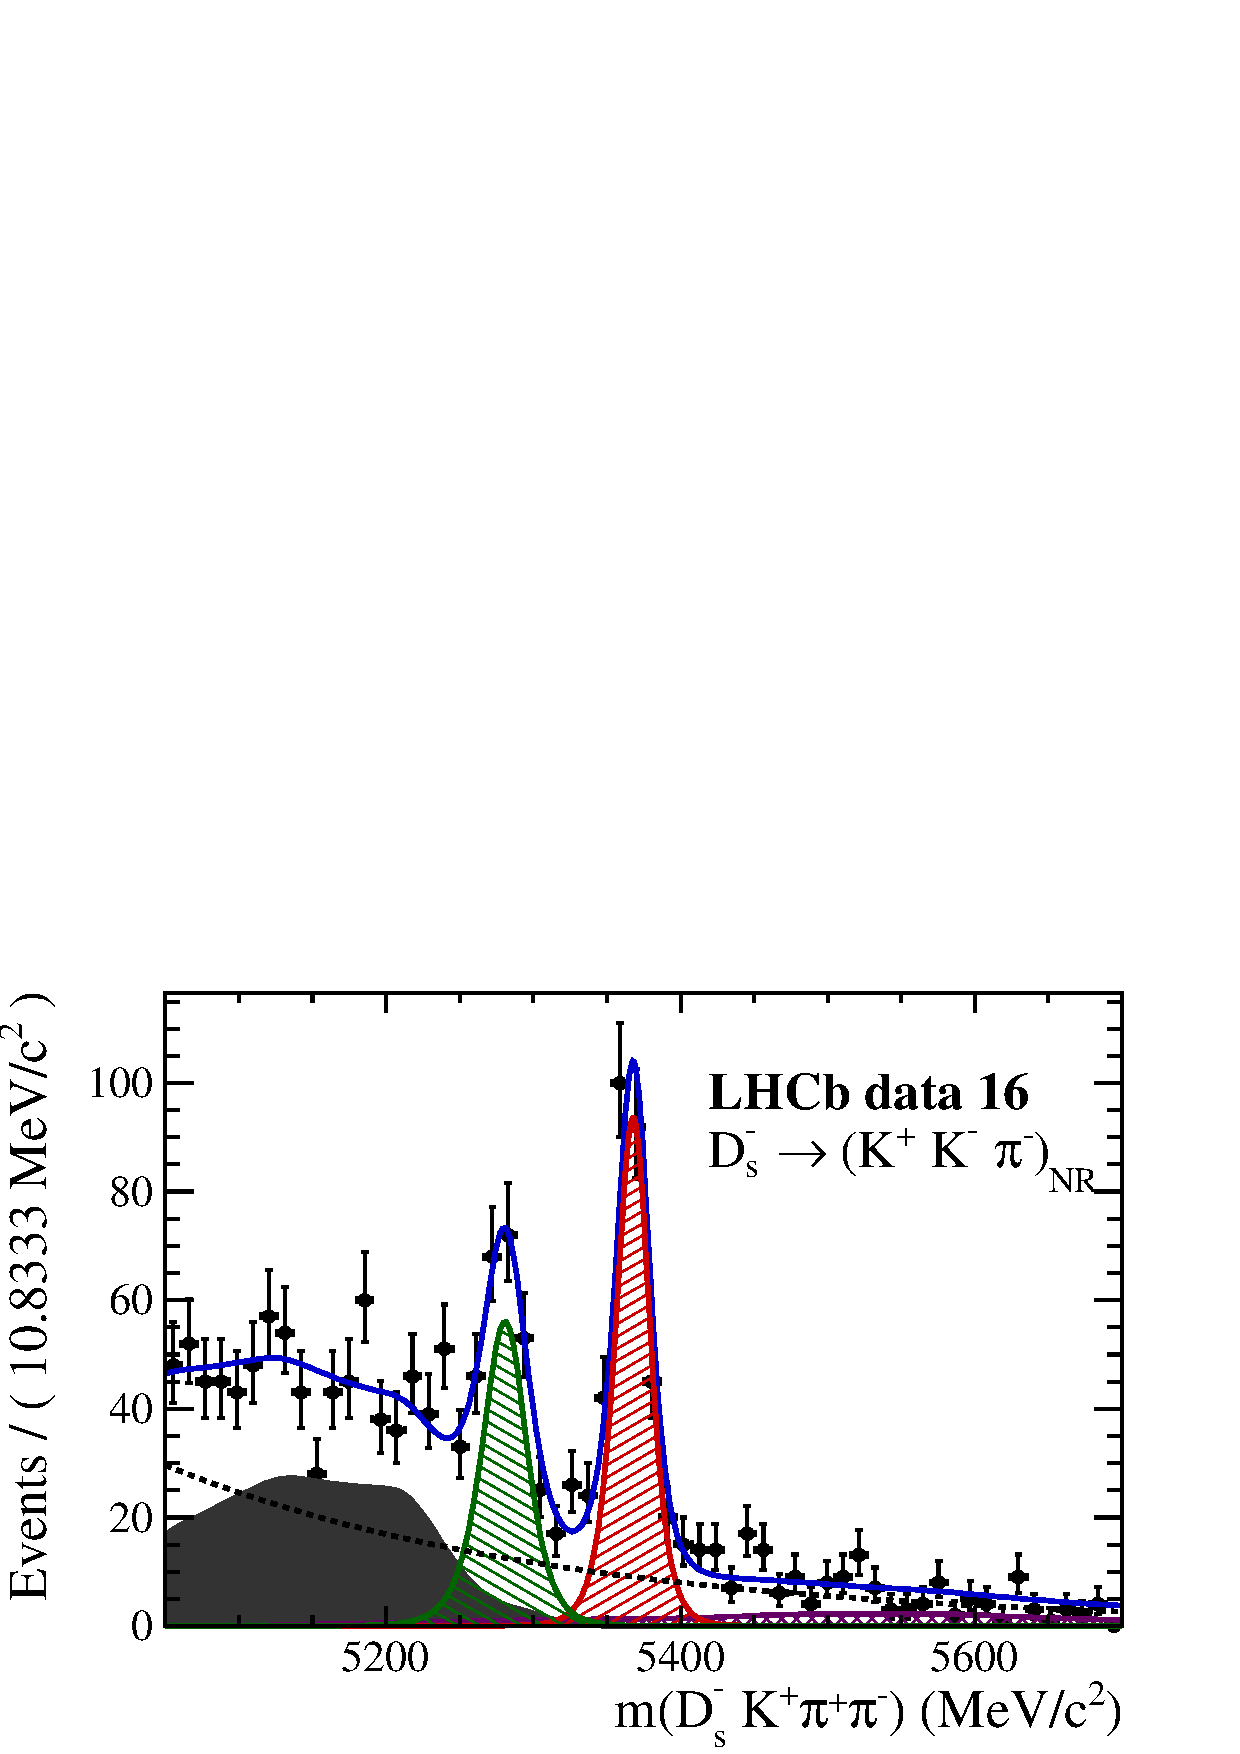
\includegraphics[height=!,width=0.5\textwidth]{figs/MassFit/signal_y16_KKpi_NR.pdf}
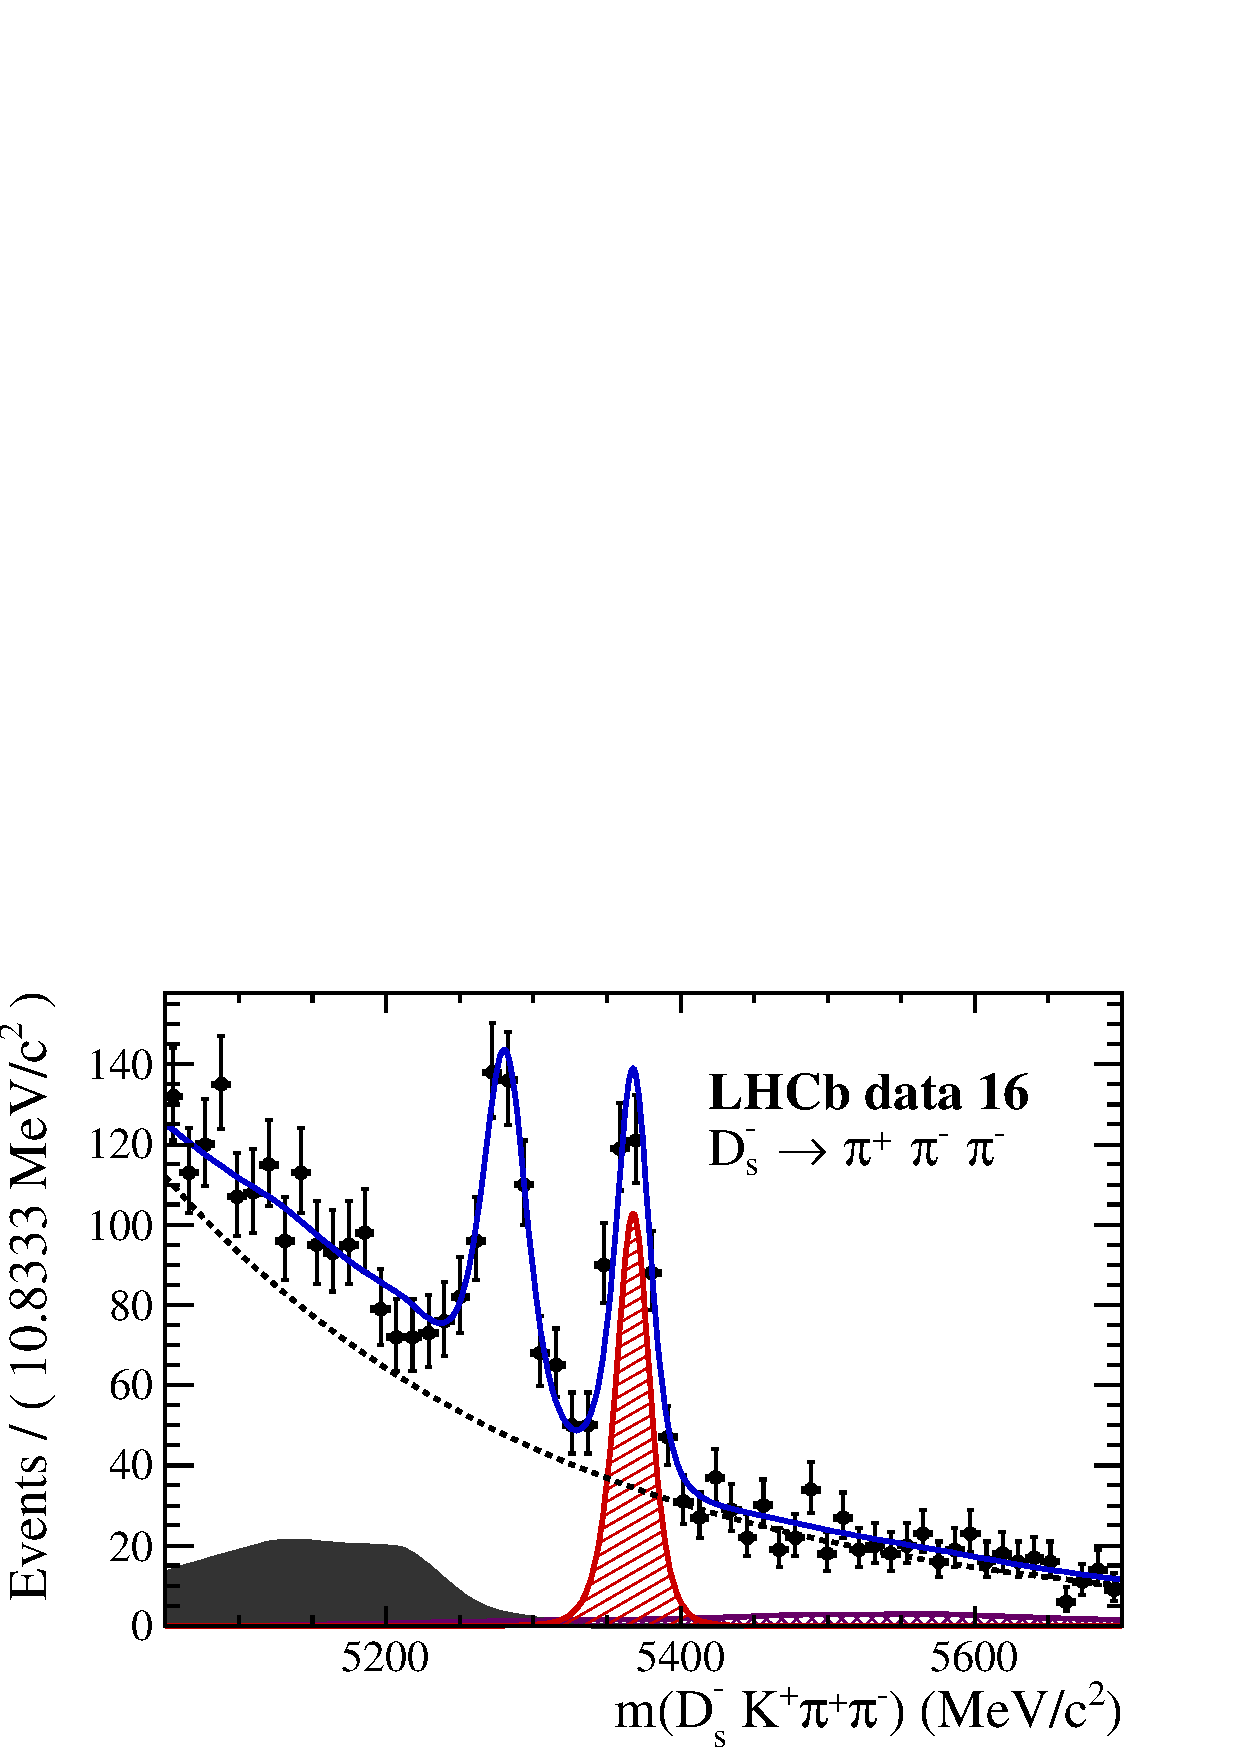
\includegraphics[height=!,width=0.5\textwidth]{figs/MassFit/signal_y16_pipipi.pdf}
\caption{Invariant mass distributions of $\Bs\to\Ds\kaon\pion\pion$ candidates, ordered by $\Ds$ final state, for Ru2 data.
The fit described in \ref{subsec: SigFit} is overlaid.}
\label{fig:massfits_signal_Run2}
\end{figure}



\subsection{Decay-time Resolution fits}
\label{subsec:DecResFits}

This section contains all fits to the distirbutions of the decay time difference $\Delta t$ between the true and the reconstructed decay time of the truth-matched $\Bs$ candidates on MC.
The fits are performed in bins of the decay time error $\sigma_{t}$, where an adaptive binning scheme is used to ensure that approximately the same number of events are found in each bin. 

\begin{figure}[h]
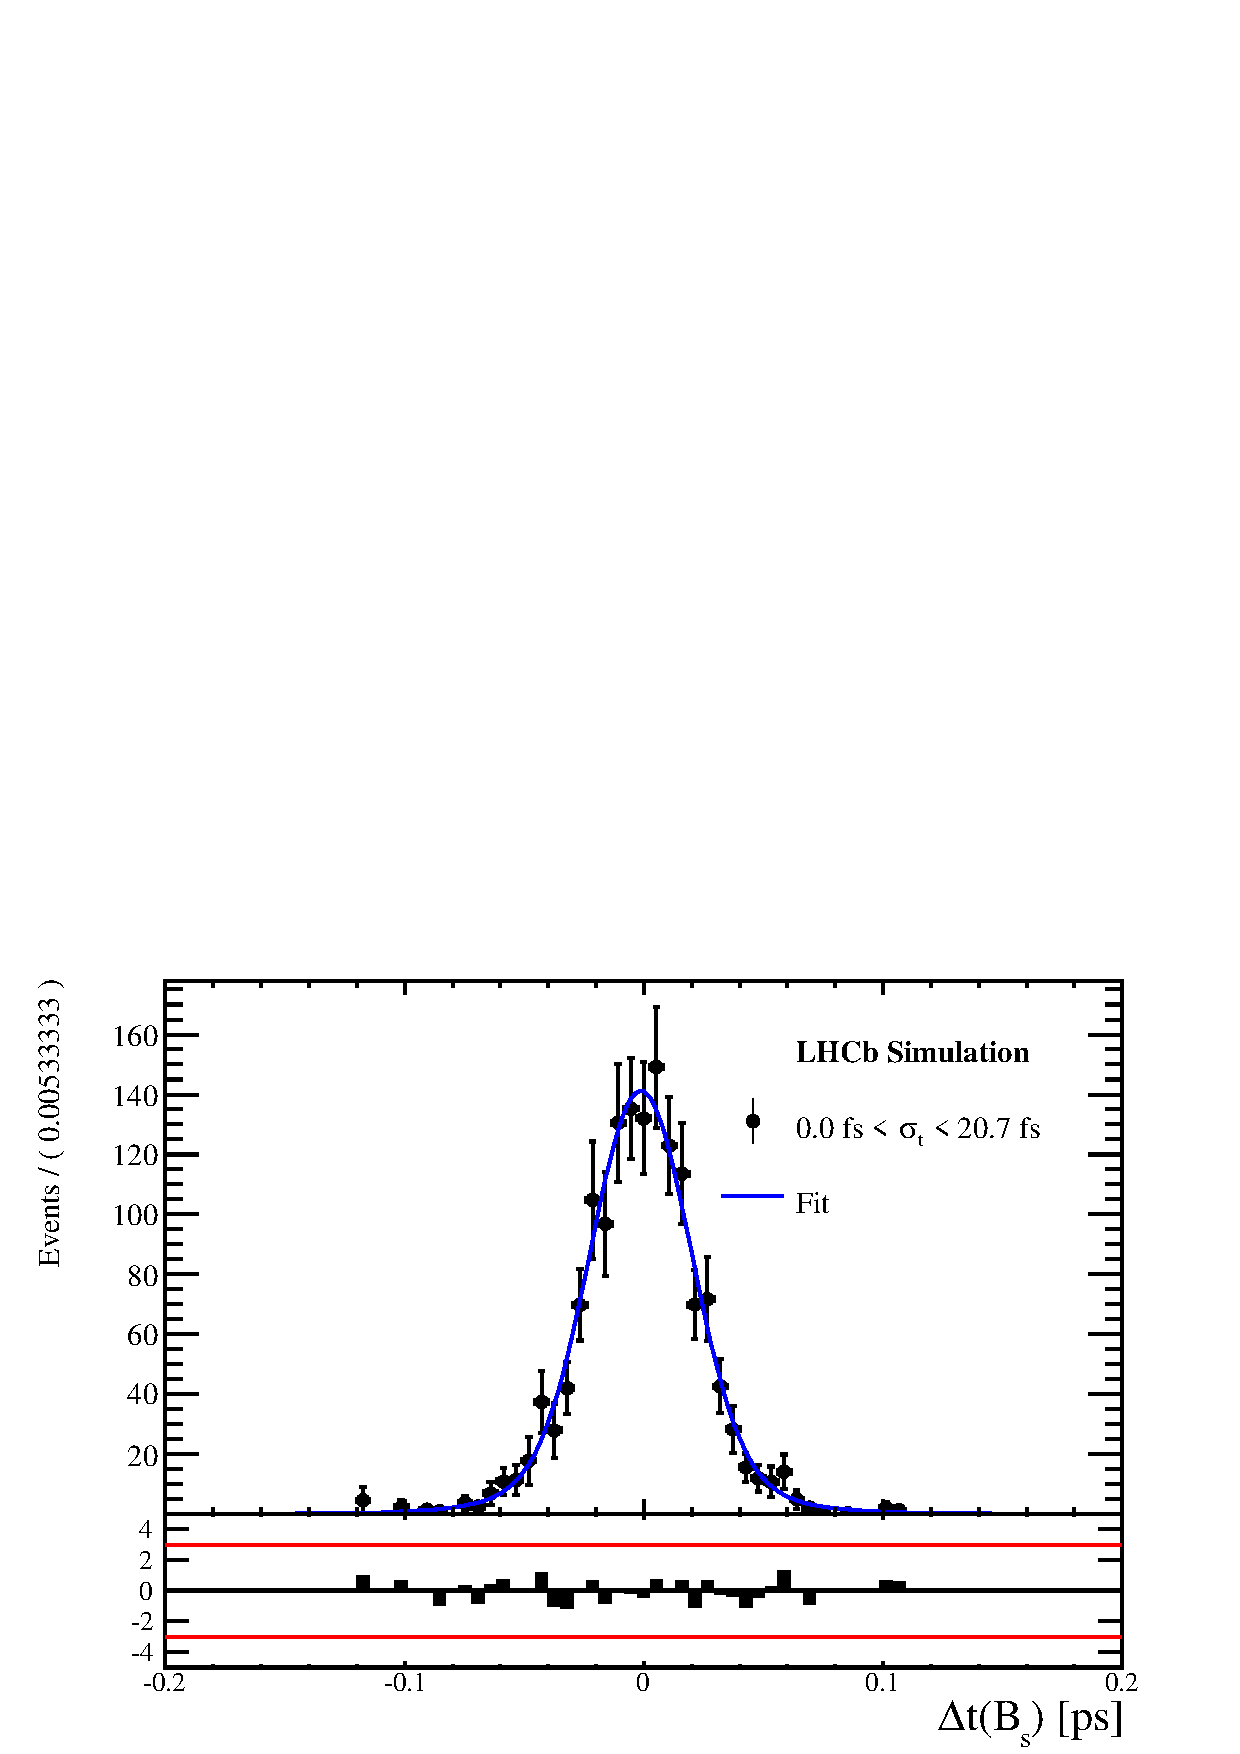
\includegraphics[height=!,width=0.5\textwidth]{figs/Resolution/SignalMC_bin_1.pdf}
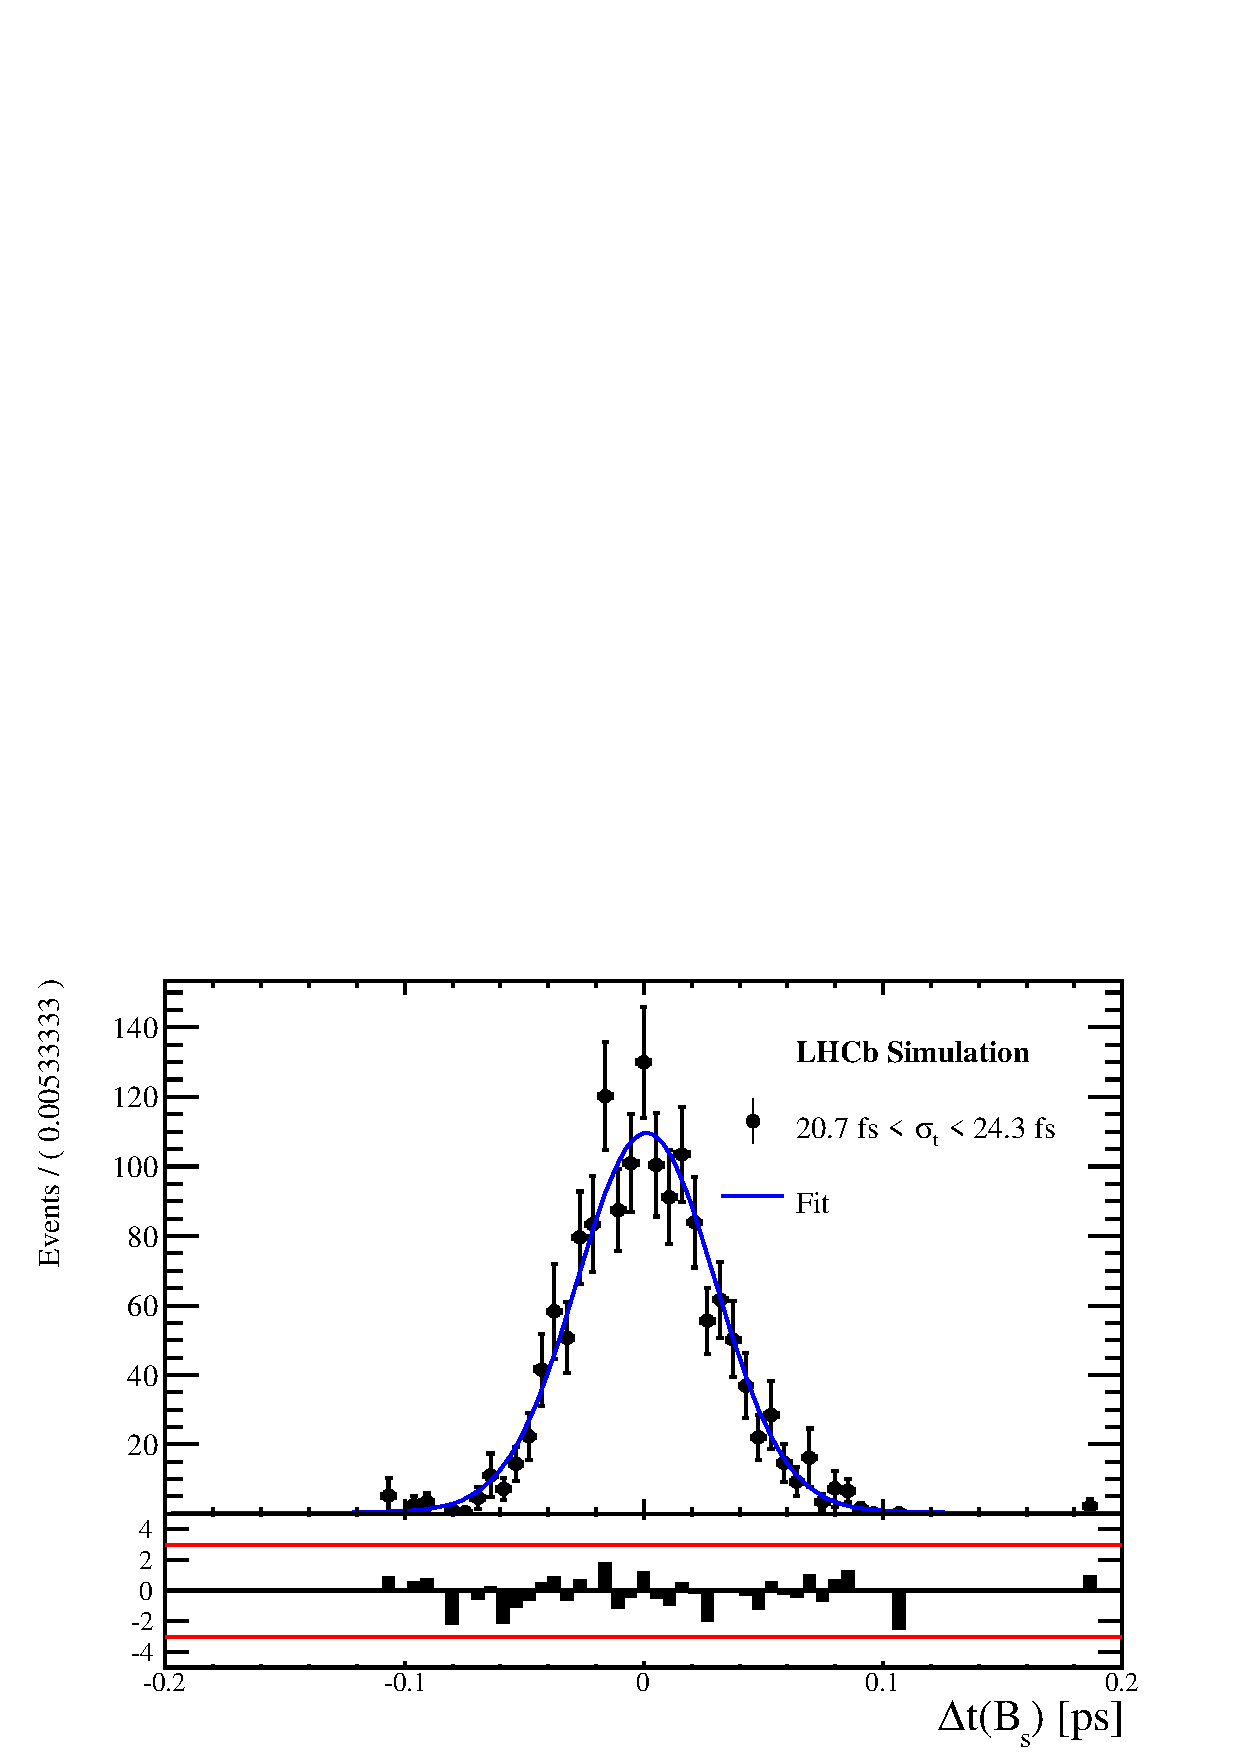
\includegraphics[height=!,width=0.5\textwidth]{figs/Resolution/SignalMC_bin_2.pdf}
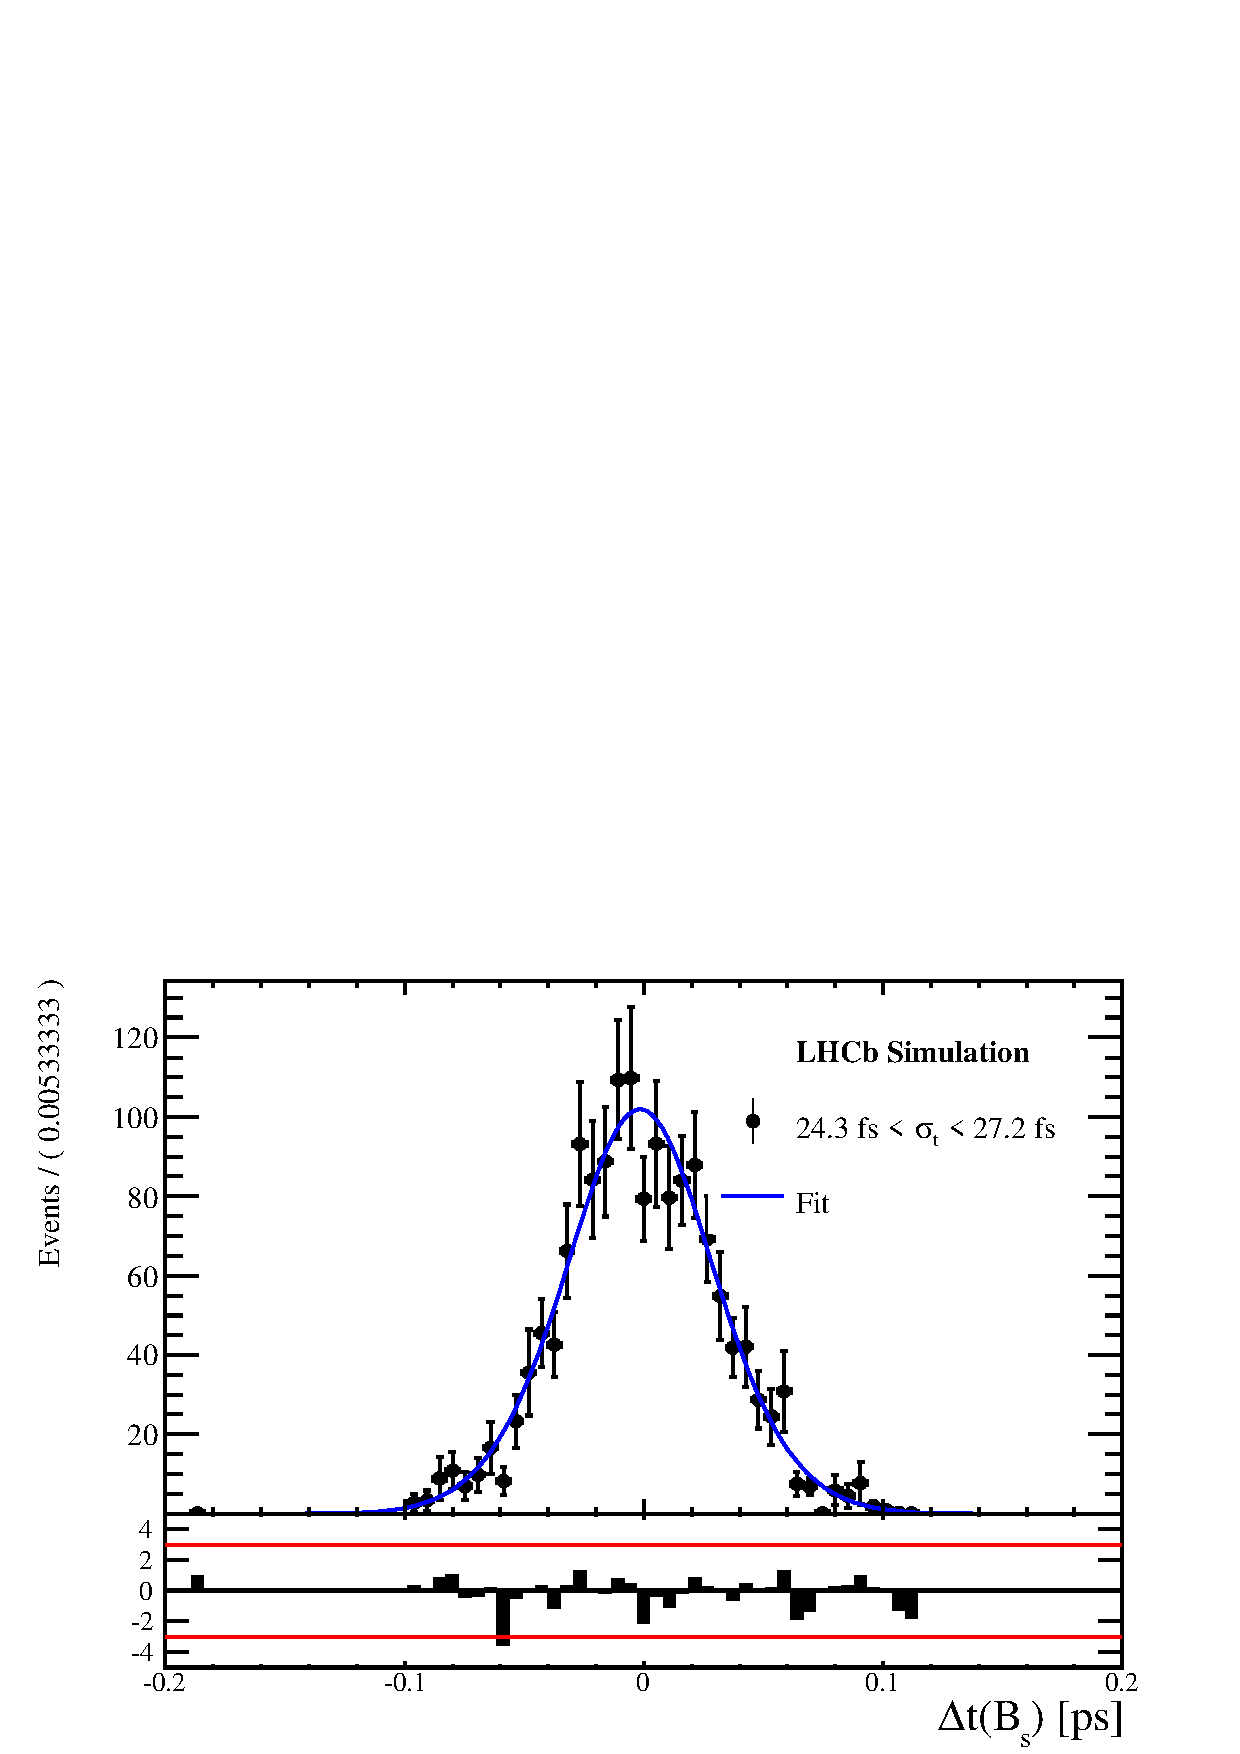
\includegraphics[height=!,width=0.5\textwidth]{figs/Resolution/SignalMC_bin_3.pdf}
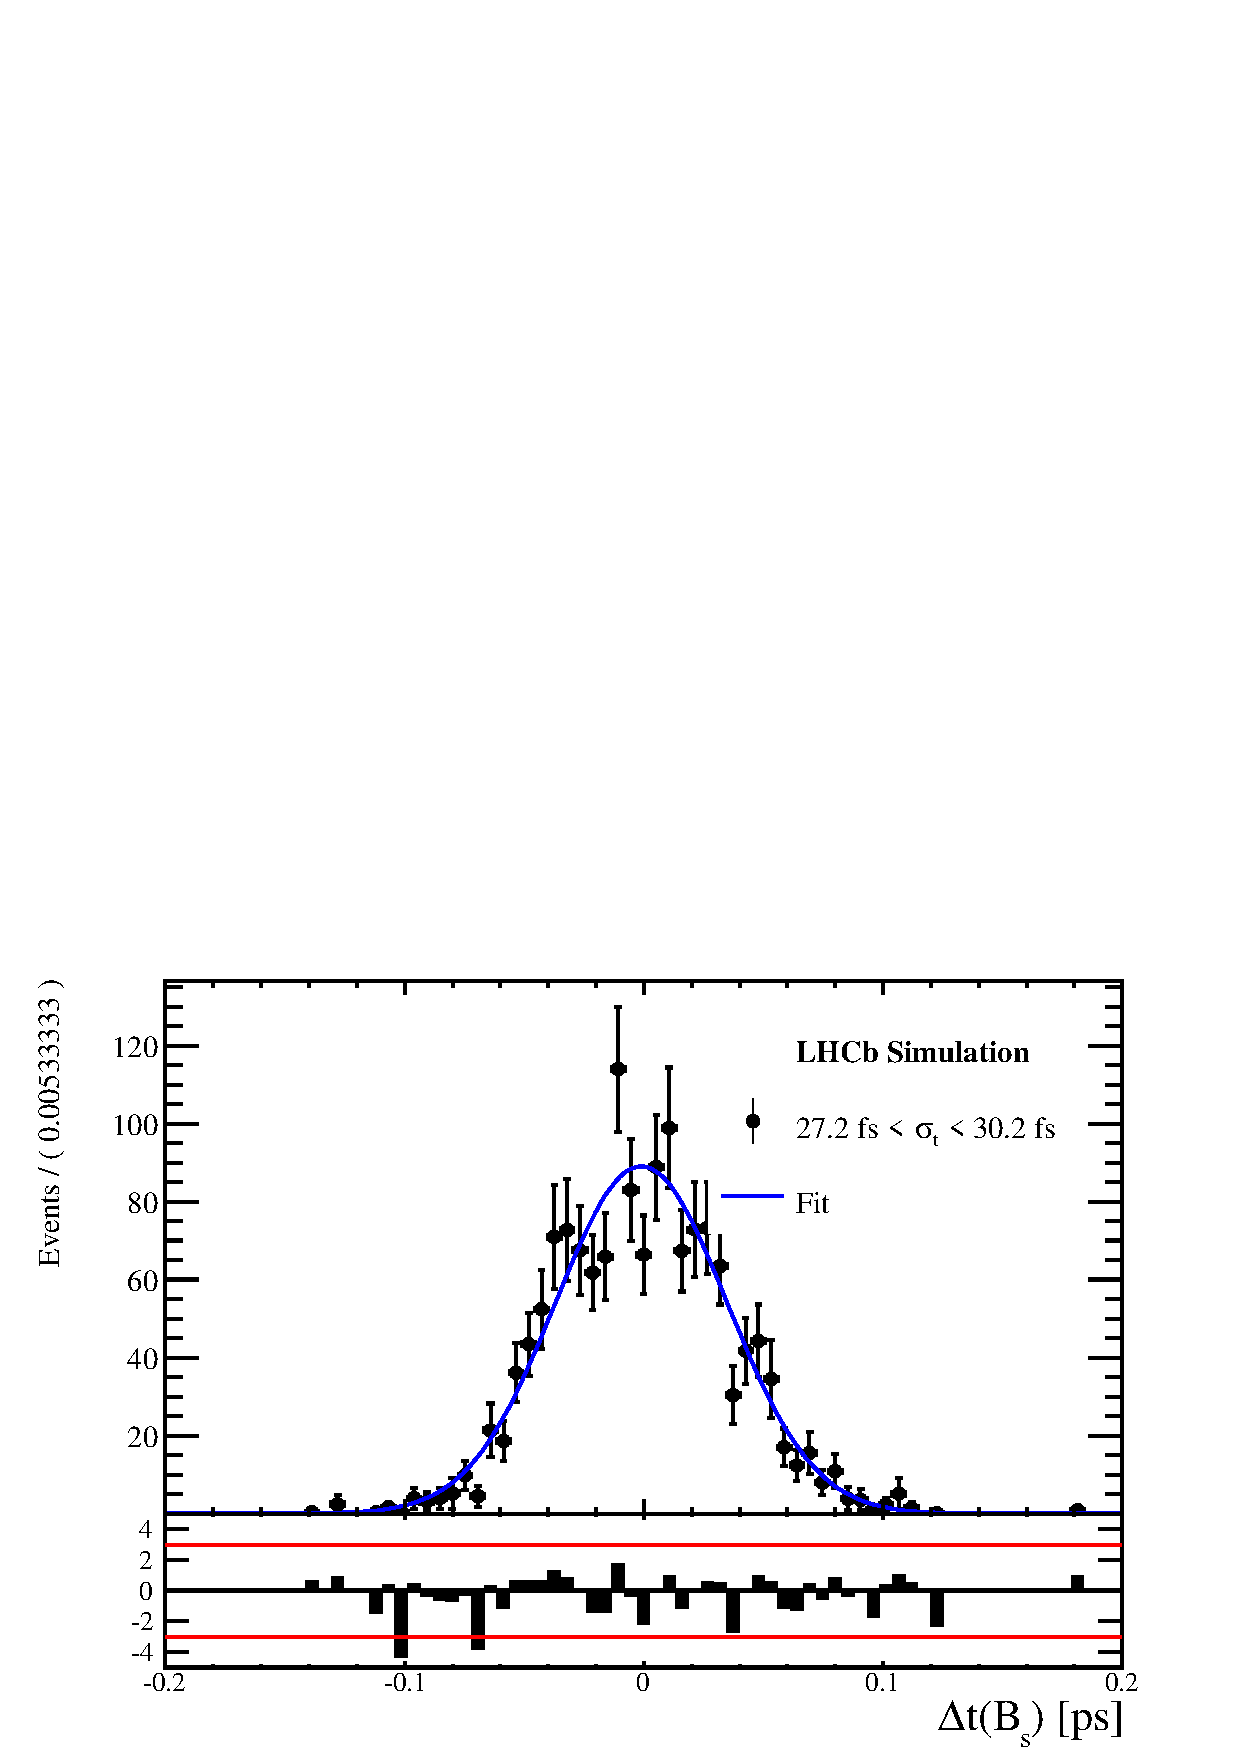
\includegraphics[height=!,width=0.5\textwidth]{figs/Resolution/SignalMC_bin_4.pdf}
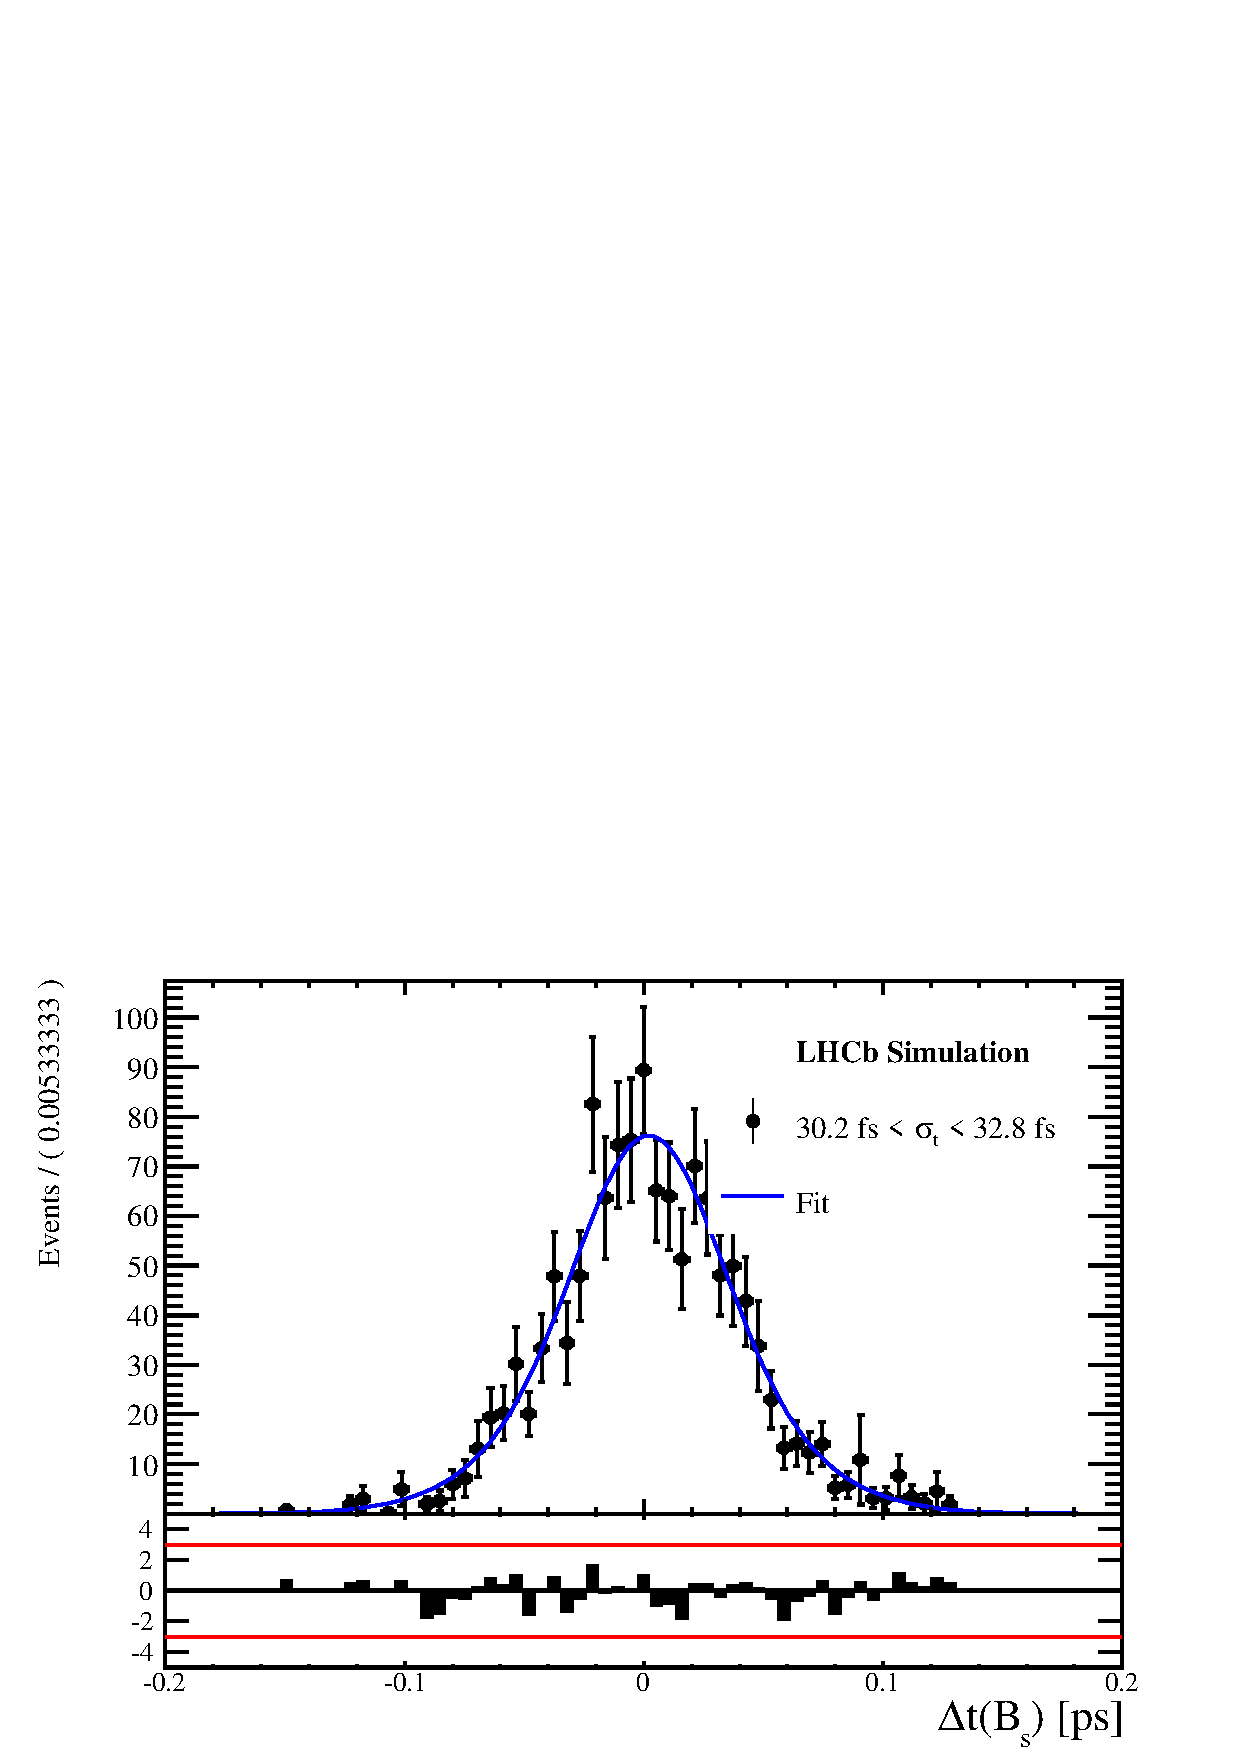
\includegraphics[height=!,width=0.5\textwidth]{figs/Resolution/SignalMC_bin_5.pdf}
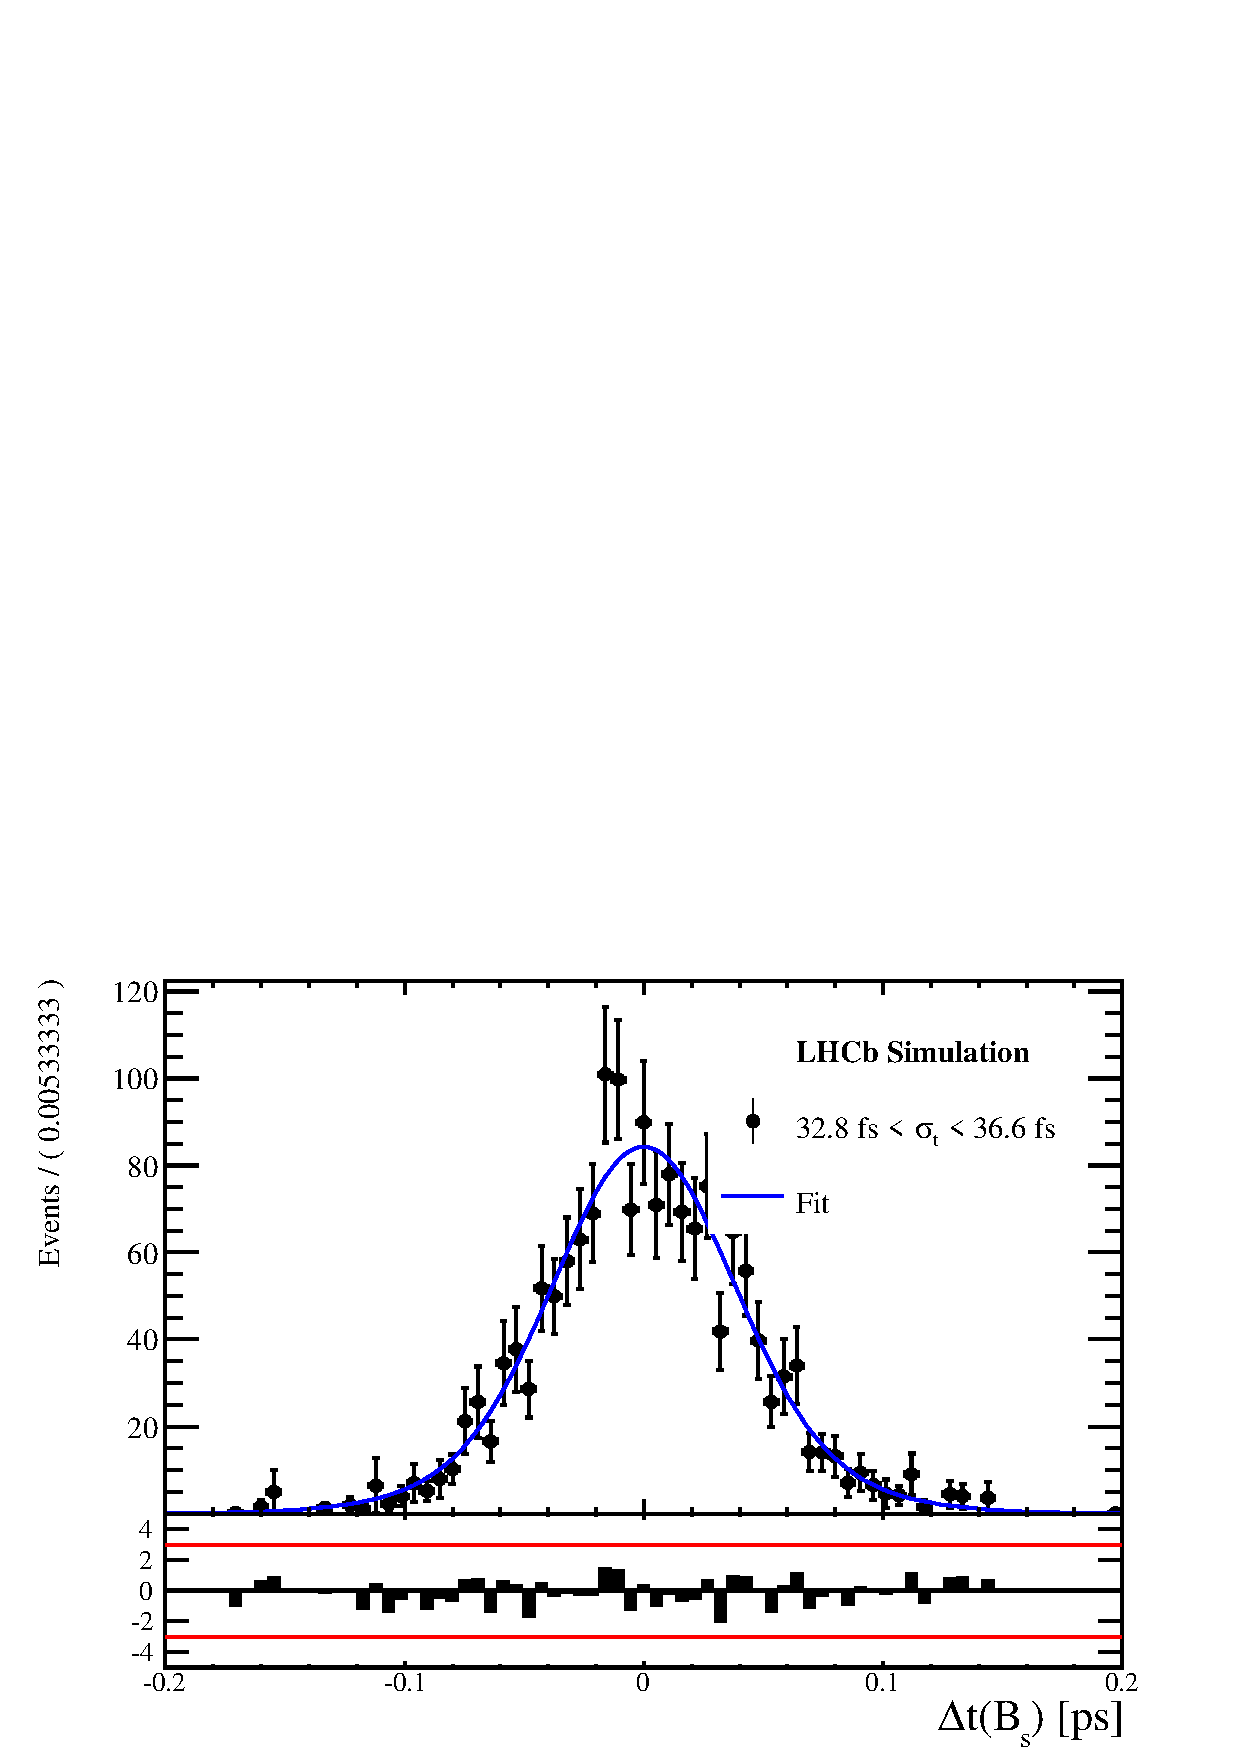
\includegraphics[height=!,width=0.5\textwidth]{figs/Resolution/SignalMC_bin_6.pdf}
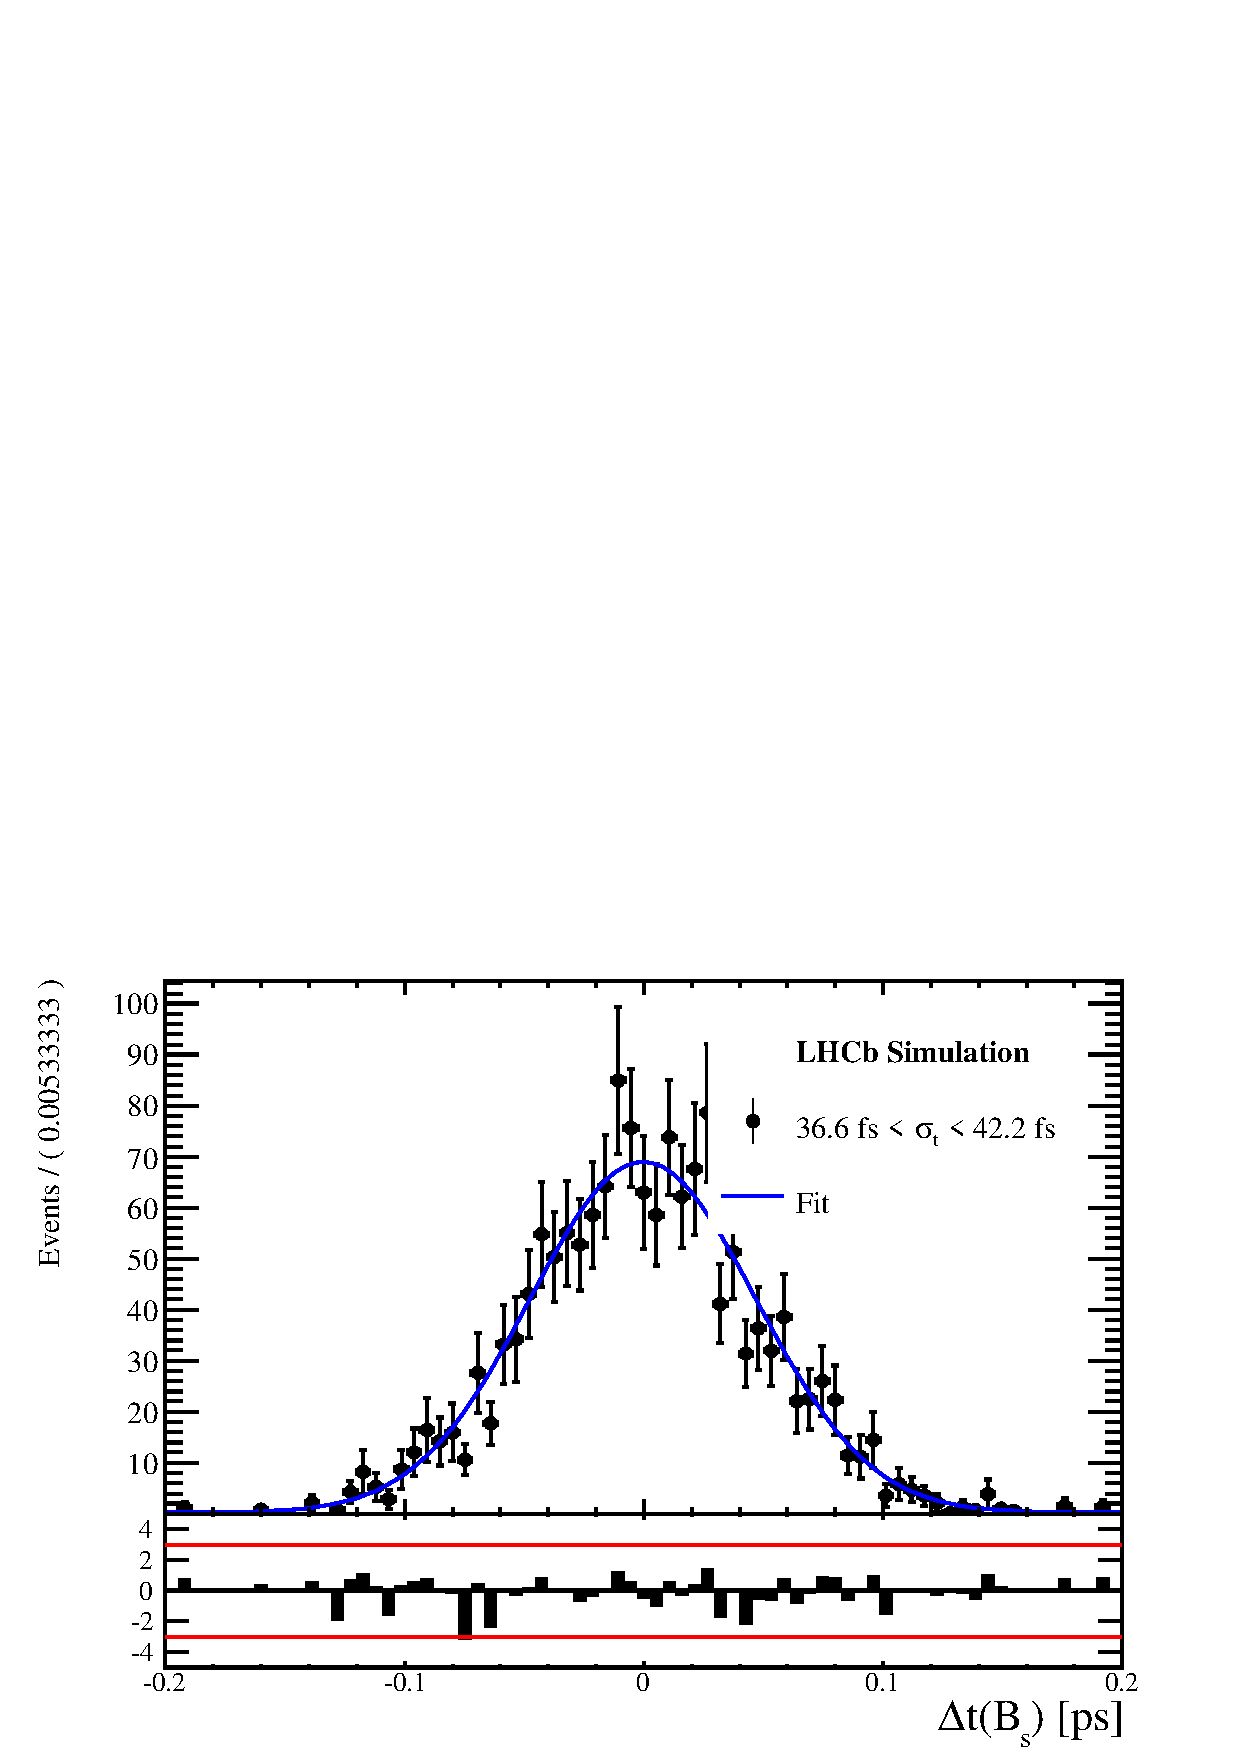
\includegraphics[height=!,width=0.5\textwidth]{figs/Resolution/SignalMC_bin_7.pdf}
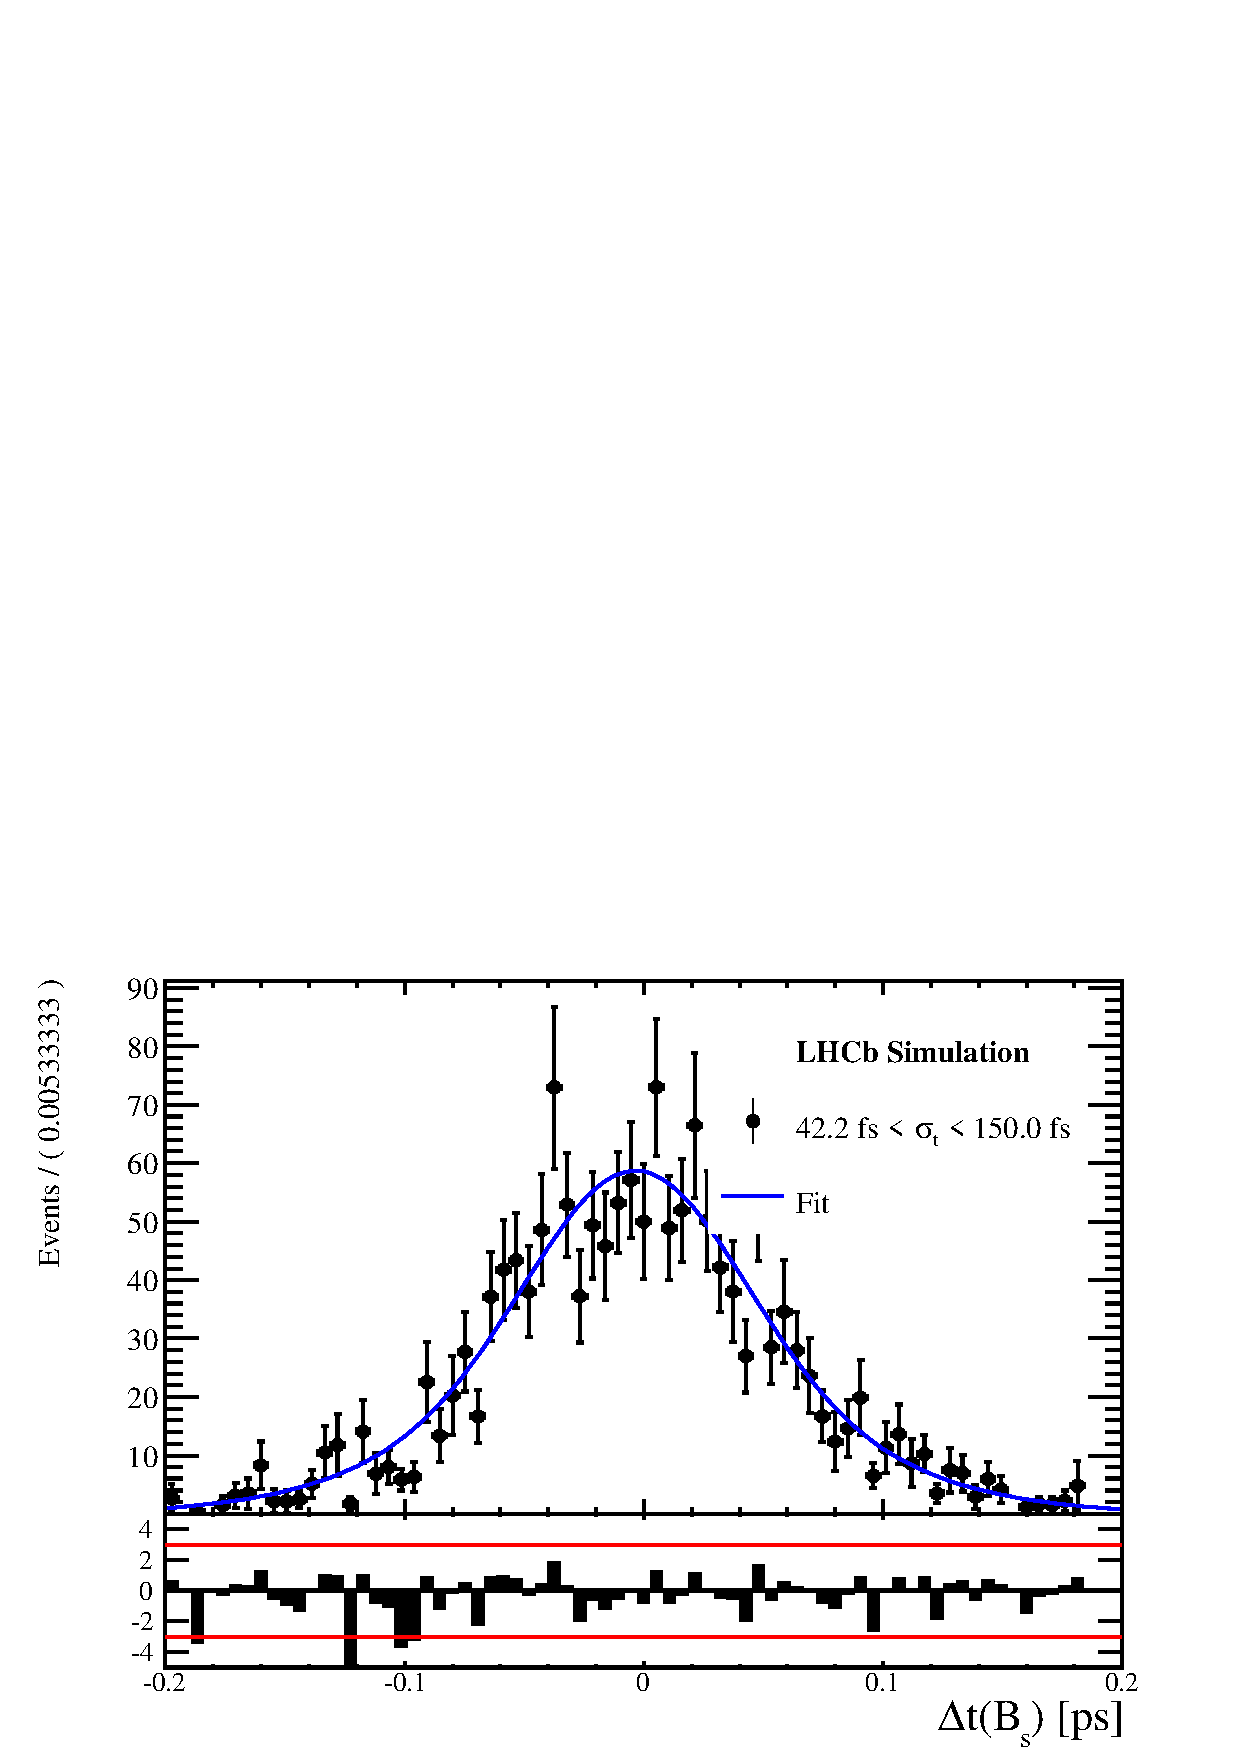
\includegraphics[height=!,width=0.5\textwidth]{figs/Resolution/SignalMC_bin_8.pdf}
\caption{Difference of the true and measured decay time of $\Bs\to\Ds\kaon\pion\pion$ candidates from MC in all bins. The fit described in \ref{sec:Resolution} is overlaid.}
\label{fig:massfits_signal_Run2}
\end{figure}
